\documentclass[abstract=on,12pt,a4paper]{scrreprt}

%PACKAGES

\usepackage[english]{babel}

\usepackage[utf8]{inputenc}% Eingabekodierung
\usepackage[T1]{fontenc}% Schriftkodierung


\usepackage{eulervm}
%\linespread{1.05}

%allows for two images in one figure and several captions
%\usepackage{subfigure}%deprecated
%\usepackage{subfig}
\usepackage{graphicx}
\usepackage{subcaption}
\DeclareCaptionFont{tiny}{\tiny} 
\captionsetup{font+=tiny} 
\captionsetup[sub]{font+=tiny} 


% For Creating Graphs and Diagrams
\usepackage{tikz}
\usetikzlibrary{shapes.geometric, arrows}
\usepackage{smartdiagram}

\tikzset{
  treenode/.style = {shape=rectangle, rounded corners,
                     draw, align=center},
  root/.style     = {treenode},
  env/.style      = {treenode},
  dummy/.style    = {circle,draw}
 
}


\tikzstyle{startstop} = [rectangle, rounded corners, minimum width=3cm, minimum height=1cm,text centered, draw=black, fill=UniVieClear!60]
\tikzstyle{arrow} = [thick,->,>=stealth]
\usetikzlibrary{shapes.multipart}

\definecolor{UniVieDark}{HTML}{005580}
\definecolor{UniVieClear}{HTML}{006699}
\definecolor{UniVieGray}{HTML}{333333}
\definecolor{UniVieOrange}{HTML}{e84e0e}

%to ennumerate Hypothesis and Research Questions.
% Not compatible with amsthm
% \usepackage[amsthm][amsmath][thmmarks]{ntheorem}
% \theoremstyle{break}
% \newtheorem{req}{Research Question}

% \theoremstyle{plain}
% \theoremseparator{:}
% \theoremindent12pt
% \newtheorem{hyp}{Hypothesis}[req]

% \renewcommand{\thetheorem}{\arabic{req}}
% \renewcommand{\thesubtheorem}{\arabic{req}.\arabic{hyp}}


% \theoremheaderfont{\sc}\theorembodyfont{\upshape} \theoremstyle{nonumberplain}
% \theoremseparator{} \theoremsymbol{\rule{1ex}{1ex}} \newtheorem{Proof}{Proof}
% \qedsymbol{\ensuremath{_\blacksquare}}

\usepackage{textcomp}
%\usepackage{mathpazo}
\usepackage{amsmath}
\usepackage{amsthm} %Not always Compatible with \ntheorem Hypothesis Numbering
%\usepackage{algorithm,algorithmic}
\usepackage[makeroom]{cancel} %package for cancel lines in formulas
\usepackage{float}
%\usepackage[noend]{algpseudocode}
\usepackage{enumitem}
\usepackage{amssymb}
%\usepackage{mathtools}
%\usepackage{a4wide}
\usepackage{fancyhdr}
\usepackage{eqnarray} 
%\usepackage{array}
\usepackage{longtable}
\usepackage{booktabs}%Tables
\usepackage[official]{eurosym} %euro symbol
\usepackage{pifont}%dingbat symbols
\usepackage[justification=centering]{caption} %forces centering of captions

\usepackage{natbib} %Bib Management

%\usepackage{cite}
\usepackage{url}

%%%%%%%%%%%%%%%
%Hypothesis
\usepackage{thmtools}
\declaretheoremstyle[
spaceabove=6pt, spacebelow=6pt,
headfont=\normalfont\bfseries,
notefont=\mdseries, notebraces={(}{)},
bodyfont=\normalfont,
postheadspace=0.6em,
headpunct=:
]{mystyle}
\declaretheorem[style=mystyle, name=Hypothesis, preheadhook={\renewcommand{\thehyp}{\arabic{hyp}}}]{hyp}

\usepackage{cleveref}
\crefname{hyp}{hypothesis}{hypotheses}
\Crefname{hyp}{Hypothesis}{Hypotheses}
%%%%%%%%%%%%%%


%\bibliography{references_MA.bib}
%\input{fano}


\usepackage[toc,page]{appendix}

%\input{primelist}

%\usepackage{pgfplots}
%\pgfplotsset{compat=1.11}

%\usepackage[left=2.5cm,right=2.5cm,top=1cm,bottom=2cm,includeheadfoot]{geometry} 

\addtokomafont{sectioning}{\rmfamily}

%UMGEBUNGEN
% \floatname{algorithm}{Algorithm}
% \renewcommand{\algorithmicrequire}{\textbf{Input:}}
% \renewcommand{\algorithmicensure}{\textbf{Output:}}

% \DeclareMathOperator{\lcm}{lcm}
% \DeclareMathOperator\ord{ord}

% \theoremstyle{definition}
% \newtheorem*{mydef}{Definition}

% \theoremstyle{definition}
% \newtheorem*{mynot}{Notations}

% \theoremstyle{definition}
% \newtheorem*{addition}{Addition Law}

% \theoremstyle{remark}
% \newtheorem*{myremark}{Remark}

\theoremstyle{plain}
\newtheorem{mytheorem}{Theorem}[chapter]

\theoremstyle{plain}
\newtheorem{myprop}[mytheorem]{Proposition}

\theoremstyle{plain}
\newtheorem{corollary}{Corollary}[theorem]

% \theoremstyle{plain}
% \newtheorem{mycor}[mytheorem]{Corollary}

% \theoremstyle{plain}
% \newtheorem{mylemma}[mytheorem]{Lemma}

% \theoremstyle{definition}
% \newtheorem*{myex}{Example}

% \theoremstyle{definition}
% \newtheorem{myconj}{Conjecture}


\newcommand{\csf}{\frac{y_i}{y_i + \sum_{j\neq i}^N y_{j}}}

\begin{document}

\begin{titlepage}
\vspace*{-2cm}  % bei Verwendung von vmargin.sty
\begin{flushright}
    
\includegraphics[width=0.5\linewidth]{Uni_Logo_2016_SW}
\end{flushright}

\begin{center}  % Diplomarbeit ODER Magisterarbeit ODER Dissertation
    \LARGE{\textbf{{\MakeUppercase{
        MASTERARBEIT / MASTER'S THESIS
    }}}}
    
    \vspace{1cm}
    \small{{  % Diplomarbeit ODER Magisterarbeit ODER Dissertation
                     % (Dies ist erst die Ueberschrift!)
        Titel der Masterarbeit / Title of the Master's Thesis
    }}
    
    \vspace{1cm}
    \Large{{  % Hier kommt der eigentliche Titel, bei Bedarf mit \\
                     % ACHTUNG: Deutsche Anfuehrungszeichen: ,,Titel``
                     %          English quotes:              ``title''
        % >>>>> BEGINN TITEL >>>>>
        ``Inequality and Social Mobility -\\
        A Laboratory Experiment''
        % <<<<< ENDE TITEL <<<<<
    }}
    
    \vspace{1cm}
    \small{{  % Verfasserin ODER Verfasser (Ueberschrift)
        verfasst von / submitted by
    }}
    
    \Large{{  % Vorname Nachname
        Hern\'an Guillermo Villamizar Maldonado, Bakk.rer.soc.oec.
    }}
    
    \vspace{1cm}
    \small{{
        angestrebter akademischer Grad / in partial fulfilment of the requirements for the degree of  % (Ueberschrift)
    }}

    \Large{{  % Magistra ODER Magister ODER Doktorin ODER Doktor
                     % ACHTUNG: Kuerzel "Mag.a" oder "Dr.in" nicht zulaessig
        Master of Science
    }}
\end{center}
\vspace{1cm}
\noindent{Wien 2020 / Vienna 2020}  % <<<<< ORT, MONAT UND JAHR EINTRAGEN
\vfill
\noindent\begin{tabular}{@{}ll}
{Studienkennzahl lt. Studienblatt /}\\
{degree programme code as it appears}\\
{on the student record sheet:}
&
\quad\quad{A 066 913}  % <<<<< STUDIENKENNZAHL EINTRAGEN
\\
&\\
    % BEI DISSERTATIONEN:
%\textsf{Dissertationsgebiet lt. Studienblatt:}
    % ANSONSTEN:
{Studienrichtung lt. Studienblatt /}\\    
{degree programme as is appears on}\\
{the student record sheet:}
&
\quad\quad{Volkswirtschaftslehre}  % <<<<< DISSGEBIET/STUDIENRICHTUNG EINTRAGEN
\\
&\\
% Betreuerin ODER Betreuer:
{Betreut von / Supervisor:}
&
\quad\quad{Univ.-Prof. Dr. Jean-Robert Tyran}  % <<<<< NAME EINTRAGEN
\end{tabular}

\end{titlepage}


\newpage
\thispagestyle{empty}
\mbox{}
\newpage

%\chapter*{Acknowledgements}

 I would like to thank my supervisor Prof. Dr. Jean-Robert Tyran for not only providing the financial support for this thesis, but also for awakening in me an interest in behavioural and experimental economics. To Dr. Axel Sonntag, who also suggested the topic for this work: thank you for providing hands-on support and for allowing open discussion throughout the entire process. Thank you also for your comprehensive feedback and for making sure the final result is the best possible version.\\

Without Milena Damrau’s help, none of the small steps needed to submit the thesis would have been possible. Thank you for your tireless moral and conceptual support throughout the duration of my Master’s studies. David Zenz has been my go-to person in all statistical issues on and off campus and this thesis has only profited from his expertise. Dr. Anja Rösner: thank you for always encouraging me and for keeping me motivated during my studies.\\

I am grateful to my family, especially my mother, Ivonne Maldonado, as well to the participants of the pilot sessions: Andres Peña, Dr. Michele Bevilacqua, and Marcela Torres.

\newpage
\thispagestyle{empty}
\mbox{}
\newpage

\chapter*{Abstract}

The present thesis lays out the design and implementation of a laboratory experiment evaluating the interplay of inequality, productivity and effort provision in a competitive setting. The design takes the form of a repeated Tullock contest where participants decide how much to work and can invest part of their earnings to increase their chances of obtaining a piece rate income above average in the next period.\\

I find that, consistent with previous research, people over-invest when participating in a rent-seeking contest. However, in my experiment, investments over the optimum decrease over time in all treatments. Against my expectations, this effect appears to be more pronounced in groups where a taxation and redistribution scheme has been implemented, in part because those groups invested nominally and relatively more than the control groups. The main driver of this effect appears to be an income effect created trough the more equally redistributed income and as a result of a fixed share of available income heuristic.\\

Probabilities of Upward Mobility grew apart with each passing round, with more participants having probabilities at each end of the distribution. The probability to win itself was determined exclusively by the available income and not, as expected, by the wage or winning status. Further cementing the idea that participants chose their investment as a share of their available income and not of their valuation of the contest.\\


\textbf{Keywords:} Social Mobility, Laboratory Experiment, Behavioral Economics\\

\textbf{JEL Codes:} 
C92 – Laboratory, Group Behavior; C72 - Noncooperative Games;
J24 - (Labor and Demographic Economics - Human Capital, Skills, Occupational Choice, Labor Productivity)\\

\newpage
\thispagestyle{empty}
\mbox{}
\newpage


\addtocontents{toc}{\protect\thispagestyle{empty}}
\tableofcontents

\textwidth15.8cm 

% \nocite{HPS08}
% \nocite{B08}
% \nocite{CP05}
% \nocite{D99}
% \nocite{P02}
% \nocite{S14}
% \nocite{AKS04}
% \nocite{PR11}
% \nocite{Ro86}
% \nocite{Mi76}
% \nocite{HR75}
% \nocite{FStatus}
% \nocite{CRXK12}
% \nocite{milne06}
% \nocite{GK99}
% \nocite{AGP94}
% \nocite{AM93}
% \nocite{LP15}
% \nocite{DB07}
% \nocite{B05}
% \nocite{TN12}
% \nocite{LN86}
% \nocite{SW}
% \nocite{GG99}
% \nocite{DPV06}
% \nocite{MO}
% \nocite{S85}
% \nocite{F85}
% \nocite{BH96}
% \nocite{wiki}
% \nocite{mersenne}
% \nocite{G04}



\pagestyle{fancy}
\fancyhead[OR]{\thepage}
\fancyhead[EL]{\thepage}
%\rhead{\fancyplain{}{\bfseries\thepage}}
\cfoot{}%keine Seitenzahl unten in der Mitte
\chapter{Introduction}
\thispagestyle{fancy}
\label{ch:intro}


Success depends in most circumstances in life not only on one's effort but on that of others. Take for instance patent races, litigation, military combat, or sports competitions, where the winner is---with varying degrees of luck involved---the one who exerted the most effort or spent the largest amount of money in comparison to the rest \citep{konrad2009}. Competitions of this sort are commonly modeled in social sciences as rent-seeking contests, as first described by \cite{tullock1980}  and expressed in a general form by \cite{sheremeta2010a}. \\

Rent-seeking contests, also called Tullock contests, are contests where the probability of winning is a function of the relative effort exerted. In their most basic form, two players compete for a price that is of equal value to both. Participants can place a simultaneous, non-refundable investment. Each of the players is then assigned a probability of winning equal to their respective share of the total investments. Meaning that if both make the same investment, each will have a 50\% chance of winning the prize. But if one invests twice the amount of the other, he or she will have a 66.33\% chance of winning.\\ 

In this thesis, I use rent-seeking contests as the base model for an economic experiment in order to better understand how inequality affects competitive behaviour in human capital investments, and how it relates to the process of social mobility. In particular I focus on whether this type of contests contribute to perpetuating inequalities and what is their impact on overall welfare.\\

With contests of Tullock type, behavioral economists can model and analyze individual and social behavior in competition and how it affects decision making. For instance, while an optimal investment strategy for this game exists, empirical examinations show that people tend to bid too much and therefore incur great efficiency losses with a median overbidding rate of 72\% \citep{sheremeta2013, chowdhury2014, konrad2009, dechenaux2015}.\\

One of the several explanations for overbidding brought forward in the literature is that winning itself has an inherent utility, separate from the utility of the prize. \cite{sheremeta2010} showed this in an experiment in which participants could invest and participate in the game, but winning did not carry a prize of positive monetary value. The prize was merely symbolic. In that study, 40\% of players invested a positive amount of money to win the prize of value 0. Moreover, participants more likely to invest in that setting, were also more likely to over-invest when a prize of positive value was offered.\\

Another common explanation is bounded rationality. Participants can make mistakes, or be confused about the rules or strategy of the game. \cite{sheremeta2011} shows, using the \textit{quantal response equilibrium} (QRE) developed by \cite{mckelvey1995}, that overbidding behaviour is consistent with bounded rationality. Subjects bids are dependent on their initial endowment amounts, rather than on the stakes of the game. While keeping the award value constant, increasing or decreasing the endowment of participants also increases or reduces the efforts of the players.\\ 

How information about other's investments and distribution levels influence a subject's investments during a rent seeking contest was studied by \cite{fallucchi2013}. In their research they find that when given full information about their own and other's decisions, over-spending by participants decreases over time to around 13\% above the optimum bid. In comparison, participants who only knew about their own efforts kept their investments high to about 63\% over the optimal level.\\

Accounting for several of these explanations simultaneously, in one of their most recent studies, \cite{sheremeta2016} shows that while overbidding is correlated with bounded rationality, systematic biases, the utility of winning and relative payoff maximization, only impulsivity remains significant in a joint multivariate analysis. Impulsive behavior was measured using the test developed by \cite{frederick2005} and known as the Cognitive Reflection Test (CRT). It aims to measure the tendency of a person to \textit{stop and think} about a question with a seemingly trivial and intuitive, but ultimately incorrect answer\footnote{A detailed description and its use in an experimental setting is given in section \ref{ss:CRT}.}.\\

\section{Social Mobility as Rent-Seeking Contest}
\label{sec:soc_mob}

Understanding the determining aspects of individual behaviour in rent-seeking contests allows us to model more complex dynamics in economics. Social mobility, for example, can be seen in many ways as a rent-seeking contest: in order to obtain a high wage position, society members exert effort trough work supply and investment in human capital. Given the limited nature of those positions, however, only a few are rewarded with the prize \citep{burkhauser2011}.\\

The results listed above might lead us to think that people tend to invest too much in their education or putting too much effort on their careers. But one crucial aspect in which social mobility in real life differs from a Tullock contest is that the outcome of the contest at a certain stage likely depends on the result of the previous stage. In other words, social mobility in practice is likely to be a series of contests in which those having won previous stages are more likely to win the next. Alumni of good schools are more likely to access the best universities, and alumni of those universities are likelier to obtain the better jobs, thus creating inequalities that may appear insurmountable \citep{sewell1971}.\\

Understanding well how the inequality arising from previous performance drives an individual's behavior is key to shaping redistribution and equality policies. Being two of the most important fields of research in economics, the literature on social mobility and inequality is equal parts massive and diverse \citep{nolan2011, atkinson2015, lipset2018, fields1999}. In this thesis I restrict myself to a model of intra-generational social mobility with only one high income position.\\ 

While there is extensive research on the effect of inequality on economic outcomes such as productivity \citep{persson1994, ku2012}, provision of public goods \citep{fehr1999} and growth \citep{ehrhart2009}, there is limited literature on how inequality affects a single agent's behaviour in a competitive setting. Does for instance a worker with lower chances of obtaining a promotion reduce her output altogether and is less likely to invest in human capital? Or does she invest \textit{too much} given the expected earnings? Generally speaking: how does inequality affect work supply and social mobility in a competitive setting?\\

\cite{fallucchi2017} studied in a laboratory setting the efforts of participants of a Tullock contest in the presence of different sources of inequality: endowment, ability, and outcomes. In all treatments participants played 30 rounds of a lottery contest. At the beginning of each round, players received an endowment of tokens that they could trade for lottery tickets, the probability of winning the round being equal to their respective share of tickets bought. The prize in tokens--plus the tokens not used to buy tickets--were stored in a separate account and payed out at the end of the experiment.\\

The baseline was a contest in which players received 95 tokens of endowment, played for a prize of 80 tokens, and where each lottery ticket costed one token. In contrast, in the treatment with \textit{inequality of endowments} one of the contestants in the group received 120 tokens while the other received only 80. In the group with \textit{inequality of ability} one of the players in each couple got one ticket per token, while the other received three. Finally, in the \textit{inequality of outcomes} treatment, the prize was of 120 tokens for one of the subjects but 40 for the other. In each of the treatments, apart from the inequality parameters, all conditions remained constant.\\

In their study, the authors find evidence that the source of inequality determines the magnitude of competitive effort put, with participants in groups with unequal abilities making larger investments than in the benchmarking case. Subjects in groups with unequal endowments or prizes, on the other hand, invested less than their counterparts in the control group. Most of this effects were driven by the disadvantaged subjects. Participants with \textit{lower} ability displayed higher effort than advantaged players, and while disadvantage subjects in the \textit{inequality of outcomes} treatment reduced their efforts, advantaged players did not increased theirs accordingly. In the same manner, an investment gap was observed in the treatment with different endowments, even though theory would predict no difference.\\

Importantly, however, the source of inequality in \cite{fallucchi2017} is exogenous. Participants are awarded more or less endowment or a higher or lower valuation randomly. But one can argue that in the case of social mobility inequality arises at least in part from success in previous performance. Better students get better opportunities in the job market and better employees are awarded higher incomes. Luck still plays a role, of course, and people who spent less effort might still win the prize. But how does it affect overall performance if the source of inequality is at least in theory meritocratic? And does success have a tendency to perpetuate itself? In the present thesis I aim to answer these questions by designing and conducting an experiment in which participants of a repeated rent-seeking contest can earn their endowments by solving a \textit{real effort task}, and subsequently invest them to increase their wages. Furthermore, I investigate the impact that a taxation and redistribution scheme has on work supply and investments on human capital.\\

Being aware that many factors will play a role in how people behave in competitions and how that translate into the results, I designed the experiment and selected model parameters in a way that presents sensible benchmarks and allows future researchers to easily change values, extend the model and devise new interventions.\\ 

\section{Social Mobility as Prospect of Upward Mobility}
\label{sec:poum}
 
To illustrate the socio-economic implications of competitive behaviour it helps to see the process of social mobility in a rent-seeking contests as analogous to a simplified version of the Prospect of Upward Mobility (POUM): the probability of achieving (or staying with) an income above average in a following period, formalized by \cite{benabou2001}. In their research the focus of the authors is primarily on the influence that the POUM has on citizens' voting behaviour. They show through theoretical considerations that when individuals decide between taxation schemes, they do so not only depending on their current social standing, but also on their probability of obtaining a higher social position in the future which helped explain the seemingly contradictory behaviour of low-income citizens voting for a reduction of taxes for higher incomes and thus against redistribution as a whole.\\

According to \citeauthor{benabou2001}, how strongly citizens approve or disprove redistribution depends in particular on the time validity of taxation and the shape of the social mobility probability function. Theorems 1 and 2 from their theoretical analysis best summarize their findings:\\
\begin{enumerate}
    \item \textit{Theorem 1:} The more concave the transition function is, the less support for redistribution among low income voters there is. Where the concavity of the transition function expresses the increasing odds of obtaining a higher income in the future with increasing current income, but at a decreasing rate.  
    \item \textit{Theorem 2:} The more "sticky" taxation policy is, or the more forward looking citizens are, the less support for redistribution there is.
\end{enumerate}

\cite{checchi2003} tested this idea in the laboratory and found strong support for it, specially the two theorems above, even after controlling for idiosyncratic factors like risk and inequality-aversion. In their experiment, subjects where randomly chosen into one of three income levels and had to decided on the taxation levels of future income based the probabilities to go from one level of income to the other. Furthermore, depending on the treatment, the taxation chosen would be applicable to one, three, or five periods.\\

The results show that for longer periods of validity of taxation, the average tax chosen by the participants declined, thus supporting the second theorem of \citeauthor{benabou2001}. In the same manner, and in line with the first theorem, when subjects were confronted with a more mobile society, i.e. the probability of transition from a lower income level to a higher one increased, they where more likely to choose a lower taxation rate.\\

An important implication of the POUM Theorem in the context of this thesis is that once a taxation scheme is in place, the POUM might be altered after redistribution if the probability of improving one's social standing depends on the redistribution result. Imagine for instance the case were the ability to invest in the training needed to rise your income depends on your previous income. If the distribution of income changes with each period, voting choices in favor or against redistribution will change accordingly, mitigating or aggravating inequality. Furthermore, if for some subjects the probability of achieving a given status becomes easier with each passing period while it becomes more difficult for others, a poverty trap can arise trough complacency or resignation at the extremes of the income distributions \citep{ceroni2001, ku2012}.

\begin{center}
  $\ast$~$\ast$~$\ast$
\end{center}

To recapitulate: in this thesis I design and conduct an experiment based on rent-seeking contests to study the effect of inequality on work supply, and investment in human capital, within an imperfect meritocratic society. Furthermore, I study how the implementation of a taxation and redistribution scheme affect mitigate or aggravate the observed behaviour. The text is presented in six parts. The introduction in this chapter motivates the thesis and offers an overview of previous research. Chapter \ref{ch:model} lays the theoretical foundation of the experiment with a formal model that generalizes \cite{koch2017}, and derives mathematical predictions that build the base of the hypotheses in section \ref{sec:hyp}. Chapter \ref{ch:experiment} presents the design and procedure of the experimental sessions, while chapter \ref{ch:results} deals with the results and their analysis. Finally, chapters \ref{ch:discussion} and \ref{ch:conclusion} conclude with policy implications, suggestions for extended research, and a short summary.

\textcolor{red}{insert summary of goal, research questions of the thesis. Interplay of social mobility and tullock contests. Insert endogenous inequality}\\
\chapter{The Model}
\label{ch:model}
\thispagestyle{fancy}

The model the experiments builds upon is inspired by \cite{koch2017} and aims to simulate a process in which an individual competes in several periods to obtain a higher wage in the next. \cite{koch2017} proposes a Tullock contest in which the relative work supply determines the probability of winning a higher income in the following period and it is described by the Contest Success Function (CSF):

\begin{equation}
    p(x_i,x_{-i}) =
\begin{cases}
    \frac{1}{n},& \text{if } x_i = x_{-i} = 0\\
    \frac{x_i}{x_i + \sum_{j\neq i}^n x_{j}},              & \text{otherwise}
\end{cases}
\label{eq:csf}    
\end{equation}

\hfill \break

Where $x_i$ is the work supplied by participant $i$ and $n$ the total number of participants. So, if a participant provides, for instance, one fourth of the total work supply, she will have a 25 percent chance of obtaining the high income in the following round.\\

This model, however, has several drawbacks. Most notably, that the probability of winning depends only on work supply and therefore redistribution has no direct effect on the Prospect of Upward Mobility. Furthermore, it allows for inequality only trough the disincentive of taxation (some participants are taxed relatively more because they earn less), and, due to the dependence between periods, is not solvable analytically.\\ 

To address those issues I consider a model where the probability of upward mobility is dependant on an individual's relative investment in human capital –similar to investment in private education.\\ 

To be precise, at the end of period $t$, an individual $i$ has the opportunity to invest an amount $I$ of her available income to increase her chances of winning a high income in the next period. Her available income is the income obtained from work after taxation and redistribution. Analogously to the case above, the Contest Success Function (CSF) is therefore defined by:

\begin{equation}
    p(I_i,I_{-i}) =
\begin{cases}
    \frac{1}{n},& \text{if } I_i = I_{-i} = 0\\
    \frac{I_i}{I_i + \sum_{j\neq i}^n I_{j}},              & \text{otherwise}
\end{cases}
\label{eq:csf}    
\end{equation}

\hfill \break

To see how a rational participant would go about deciding her optimal investment, let us consider the simplest case of a game with two periods where the share of total investment at the end of the first period determines the probability of obtaining the prize of a high wage in the second according to the CSF.\\

In the second period, the last in this case, exactly one participant will have a high wage $w_h$ while all others will work with a low wage $w_l$. That means that a participant $i$'s prize, or valuation $\mathbb{V}$ of the game, is equal to the difference in earnings between what she would earn with the high vs. with the low wage. At the end of the first period, participant $i$ has then to choose how much to invest in order to maximize the chances of obtaining the prize $\mathbb{V}$.\\

In period 1 a participant wants therefore to maximize her expected profit $\mathbb{E}\Pi_i$ according to the optimization problem:

\begin{equation}
    \underset{I_i}{\text{max}}\quad\mathbb{E}\Pi_i(I_i,I_j) = \frac{I_i}{I_i + \sum_{j\neq i}^n I_{j}}\mathbb{V} - I_i
\label{eq:exp_util}
\end{equation}

Assuming risk-neutrality and that the valuation $\mathbb{V}$ of the higher wage is equal for all participants and therefore that $I_i^{*}=I_{-i}^{*}=I^{*}$ it can be easily shown that the optimal investment amount is:

\begin{equation}
    I^{*} = \frac{n-1}{n^2}\mathbb{V}
\label{eq:opt_last}
\end{equation}

\hfill \break 

The optimal amount of investment in the first round will hence depend inversely on the number of participants and directly proportional to the value of the prize.\\

\subsection{Ensuring Opportunity: The Budget Constraint}
\label{sec:budget_constraint}

But what happens if there are several consecutive rounds? In the presented design, the probability of obtaining the high income in the next period is independent from the previous period only if the optimal investment amount is higher than the available income. In other words, if a participant that has not won the high wage cannot afford the optimal investment, he would have an increased interest to earn the high wage in previous periods. The budget constraint $\frac{n-1}{n^2}\mathbb{V} \leq \pi(w_l)$ is thus violated whenever $\frac{\pi(w_h)-\pi(w_l)}{\pi(w_l)} > \frac{n^2}{n-1}$.\\

Pilot sessions have shown that in a game with three participants, a high wage of approximately five times the low wage will make it impossible for a low wage participant to invest the optimal amount. I take this into account for the current experimental design and make the high wage only twice as large.

\subsection{Asymmetric Valuations}

An important conundrum that the here presented approach makes easier than \cite{koch2017} to solve is a possible difference in valuation of the prize in terms of higher wage since participants with higher ability or higher utility from consumption will have a higher profit from it. \cite{nti1999} shows that in the two player case:\\

\begin{quote}
    "The player who values the prize more expends more effort in equilibrium but both players allocate the same fraction of their valuations to the contest"\footnote{\cite[p.~419]{nti1999}}.
\end{quote}

To show this, we just need to write the FOC for the two players explicitly:

\begin{equation*}
\begin{split}
    \frac{I_j}{(I_j + I_i)^2}\mathbb{V}_i-1 = 0 \\
    \frac{I_i}{(I_j + I_i)^2}\mathbb{V}_j-1 = 0
\end{split}
\end{equation*}

Equalizing we obtain:
\begin{equation}
    \frac{I_i}{\mathbb{V}_i} = \frac{I_j}{\mathbb{V}_j} 
\end{equation}

Now let us consider the case of $n=3$ for $i \in (a,b,c)$. Using the same process as above we obtain the equation system:

\begin{align}
    \frac{(I_a+I_b)}{(I_a+I_b+I_c)^2}\mathbb{V}_c&=1\\
    \frac{(I_a+I_c)}{(I_a+I_b+I_c)^2}\mathbb{V}_b&=1\\
    \frac{(I_b+I_c)}{(I_a+I_b+I_c)^2}\mathbb{V}_a&=1
\end{align}

To easier visualize the results we assume w.l.o.g that $I_a = I$, $I_b = \beta_b I$ and $ I_c = \beta_c I $, and that $\mathbb{V}_a = \mathbb{V}$, $\mathbb{V}_b = \alpha_b \mathbb{V} $ and $\mathbb{V}_c = \alpha_c \mathbb{V}$. The equation system thus is simplified to:

\begin{align}
    \label{eq:sys1}\frac{(1+\beta_b)}{(1+\beta_b+ \beta_c )^2}\alpha_c\mathbb{V}&=I\\
    \label{eq:sys2}\frac{(1+\beta_c )}{(1+\beta_b  + \beta_c )^2}\alpha_b\mathbb{V}&=I\\
    \label{eq:sys3}\frac{(\beta_b +\beta_c )}{(1+\beta_b  + \beta_c )^2}\mathbb{V}&=I
\end{align}

After setting (\ref{eq:sys2}) = (\ref{eq:sys3}) we obtain:

\begin{equation}
    \label{eq:betab}\beta_b=(1+\beta_c)\alpha_b-\beta_c
\end{equation}

Similarly, we set (\ref{eq:sys1}) = (\ref{eq:sys3}) and obtain $(1+\beta_b)\alpha_c=\beta_b+\beta_c$ in which we can replace $\beta_b$ by (\ref{eq:betab}). Solving for $\beta_c$ we get:
\begin{equation}
\label{eq:betac}
    \beta_c = \frac{\alpha_b-\alpha_c-\alpha_b\alpha_c}{\alpha_b\alpha_c-\alpha_c-\alpha_b}
\end{equation}
Which inserted back in (\ref{eq:betab}) gives us:
\begin{equation}
\label{eq:betab2}
    \beta_b=\alpha_b + \alpha_b\frac{\alpha_b-\alpha_c-\alpha_b\alpha_c}{\alpha_b\alpha_c-\alpha_c-\alpha_b}-\frac{\alpha_b-\alpha_c-\alpha_b\alpha_c}{\alpha_b\alpha_c-\alpha_c-\alpha_b}
\end{equation}

Finally, from (\ref{eq:betab2}) and (\ref{eq:betac}) we know that $\beta_b+\beta_c = 1+\alpha_b\frac{\alpha_b-\alpha_c-\alpha_b\alpha_c}{\alpha_b\alpha_c-\alpha_c-\alpha_b}$ and we can replace in \ref{eq:sys3} to obtain:

\begin{equation}
\label{eq:InvDiffVal}
    I = \frac{\alpha_b+\alpha_b\frac{\alpha_b-\alpha_c-\alpha_b\alpha_c}{\alpha_b\alpha_c-\alpha_c-\alpha_b}}{(1+\alpha_b
    +\alpha_b\frac{\alpha_b-\alpha_c-\alpha_b\alpha_c}{\alpha_b\alpha_c-\alpha_c-\alpha_b})^2}\mathbb{V}
\end{equation}

\hfill \break

Now, to more easily see how this function behaves let us assume that only participant \textit{c} has a different valuation and therefore $\alpha_b = 1$. It follows:

\begin{equation}
    I_a=I_c=\frac{2\alpha_c}{(1+2\alpha_c)^2}\mathbb{V}
\end{equation}

The denominator will grow faster for increasing $\alpha_c$ which means that $I_a$ will tend to $0$.\\


The general case is more cumbersome but we can still find some conditions for the relationship between $\alpha_b$ and $\alpha_c$. Requiring that $\alpha_b, \alpha_c \in \mathbb{R}^+$ and that $\alpha_b\alpha_c-\alpha_c-\alpha_b \neq 0$, it can be shown that, in order for $I\geq0$, then $\alpha_b\alpha_c>\alpha_c+\alpha_b$.\\

This means in particular that there are some levels for which an investment is no longer profitable, take for instance $\alpha_b = 2$ and $\alpha_c = 4$.\\

A look at the function graph \ref{fig:invest_func} gives us a better intuition of its behavior. For very low levels of others' valuations the investment value is close to zero but increases with $\alpha_b$ and $\alpha_c$. After achieving a maximum of $\frac{1}{4}$, or the equivalent to the two player game, the function decreases monotonically.

\begin{figure}[H]
    \centering
    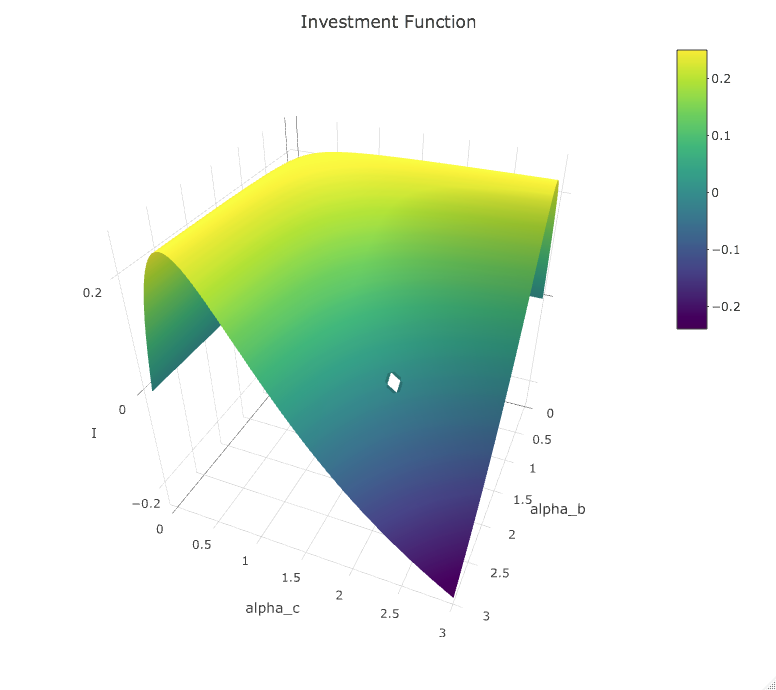
\includegraphics[scale=0.5]{graphs/Investment_Func.png}
    \caption{Investment function dependant on the share of others' valuation}
    \label{fig:invest_func}
\end{figure}

\subsection{Theoretical Predictions}

Regardless of the repetitions of the game, the expected profit maximizing investment for a given player is constant as, first, the valuation of the game is constant across periods, and, second, the invested amount only affects the winning probabilities of the subsequent period.\\

Furthermore, since work supply does not enter the CSF and, as explained in section \ref{sec:budget_constraint}, participants can always afford to invest their optimum, there is no incentive to work more than the profit maximizing amount.
    \chapter{Experimental Design}
    \label{ch:experiment}
    \thispagestyle{fancy}
    
    To empirically test the theoretical statements of the model described in chapter \ref{ch:model}, I designed and conducted a laboratory experiment. The current chapter begins with a general overview in section \ref{sec:gen_str}. It then lists the considerations going into the selection, design and parametrization of the Real Effort Task (RET) in section \ref{sec:RET} and then details all the steps and screens in the chronological order in which each element is presented to participants. The goal here is to make explicit which information is available to players at each moment during the experiment.\\
    
    The treatment intervention is explained in section \ref{sec:treat}, while the hypotheses derived from this specific design and the research question proposed in the introduction chapter are laid out in section \ref{sec:hyp}.
    
    \section{General Structure of the Experiment}
    \label{sec:gen_str}
    
    The general goal is to let players invest their earnings from solving a Real Effort Task to increase their individual chances to win a contest awarding the double wage in the following round as explained in the theoretical model of section \ref{ch:model}. This process is repeated several times with the same participants in each group and round.\\ 
    
    % To avoid having a situation where wage increase does not result in effort increase, paid leisure is introduced. How paid leisure works is explained in detail in subsection \ref{ss:switch_mode}.\\
    
    The experiment is roughly divided into three sections as shown in figure \ref{fig:exp_str}\footnote{ Table \ref{tab:exp_design} in the appendix lists a detailed breakup of the three main sections and its contents}. The first is an introductory section where the principal components of the experiment, including the RET, are explained in great detail to the participants. In this first section, participants are also asked several control questions to test for their understanding of the task.\\
    
    Within the introductory section, participants complete two rounds of the RET, once with a low payment per task and once with a high payment per task. This is used later as a baseline against which the performances in the competitive rounds are compared. An in detail description of each step and screen during the introductory section is written in section \ref{sec:intro_exp}.\\
    
    The second section is the Tullock competition and it is the core of the experiment. In it, participants earn money by solving the RET which they can subsequently invest to win a higher piece rate in the following round.\\
    
    Finally, in the third section participants answer several questionnaires regarding their demographics, their cognitive reflection and their risk aversion.\\
    
    \begin{figure}
\centering
\begin{tikzpicture}
  [
    grow                    = right,
    level distance          = 8em,
    edge from parent/.style = {draw, -latex},
    every node/.style       = {font=\footnotesize}
  ]
  \node(0) [root] {Instructions \&\\ Benchmark}
    child {node [env](ret) {RET}
                child{node[env]{Investment}
                    child{node[env](award){Award}
                        child{node[env]{Demographics \& \\ Control}
                    }
                }
            }
        };
      
      
    %draw the arrow from award to RET
    \draw[->]  (award) -- node {} ++(0,1cm) -| 
        (ret) node[pos=0.25, above] {High/Low Wage(8x)} 
        node[pos=0.75] {};
    
    
\end{tikzpicture}

\caption{Basic Structure of Experiment}
\label{fig:exp_str}
\end{figure}
    
    The experiment was programmed using oTree \citep{chen2016}\footnote{A playable demo version is available at \textcolor{red}{XXX.XXX.XXX}}, and was conducted at the \textit{Vienna Center for Experimental Economics}. Participants were not allowed to communicate, nor to use their cellphones. The instructions were presented to all participants on-screen and were also read aloud to let them know everyone had the same information. Also, at every step during the instruction reading, participants were actively asked if they had any questions and we only proceeded if no one had. Lastly, participants were paid anonymously at the end of the session, in private, and in cash.
    
    
    \section{Real Effort Task}
    \label{sec:RET}
    
    The RET is inspired by \cite{rey-biel2016} and \cite{giusti2014}. Participants are asked to count the occurrences of the letter ``a'' in a random string of characters. Figure \ref{fig:LC_screen} gives an example of such a string which in the experiment is called a \textit{sequence}. The sequence is generated pseudo-randomly but it is identical for every participant in the session. A fact that all participants are made aware of.\\ 
    
    \begin{figure}
        \centering
        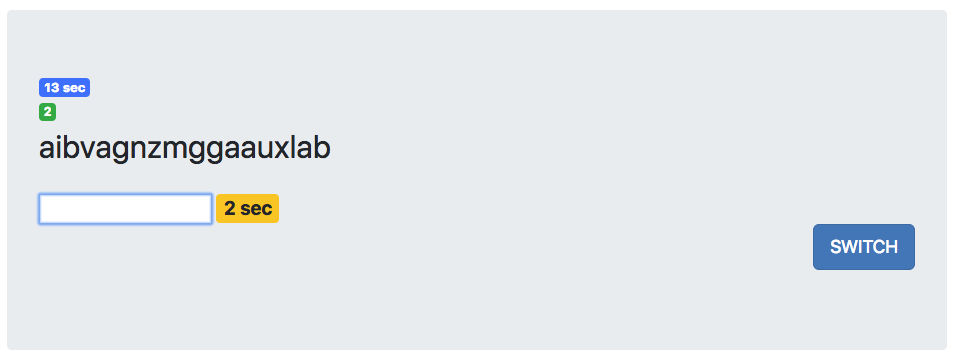
\includegraphics[width=\textwidth]{graphs/screenshot_RET_alone.png}
        \caption{Sample Screen of the Letter Counting Task}
        \label{fig:LC_screen}
    \end{figure}
    
    This particular task has been chosen as it fulfills several requirements from my design. The main research questions address the effects of inequality on performative measures like output, and efficiency. To be able to observe changes in those measures it is therefore important to ensure that participants are not simply always doing as much as they can, i.e. a corner solution. Such a phenomenon would be particularly strong if players have a strong intrinsic motivation or if no incentive is offered to stop solving tasks \citep{frey1997}. An example of a task with high intrinsic motivation would be any fun game as, for instance, Tetris.
    The Letter Counting Task is tedious and repetitive without being effortless and therefore offers a particularly strong effect for monetary incentives \citep{cerasoli2014}.\\
    
    Furthermore, the task is easy to explain and it does not rely on a mathematical framing which has been shown to induce a gender gap, when in a competitive setting, not linked to skill \citep{niederle2010}.\\ 
    
    Note also, that every time before the Real Effort Task (RET) starts, a waiting page makes sure that all participants have completed all sections before, thus avoiding some participants solving the task while others read. Also, a confirmation page is displayed before the start of the RET so that participants are not taken by surprise.
    
    \subsection{Incentivised Leisure}
    \label{ss:switch_mode}
    
    Another issue present when trying to identify work supply levels in the laboratory that might produce a corner solution is the missing of incentivisation of non-work. In real life, leisure has an intrinsic motivation which in economics is quantified by the opportunity costs of not working. In the laboratory, however, due to the short time frame, implicit peer pressure and possible experimenter demand effects, participants might be averse to stop supplying work and spend time in leisure. To address this issue, a fundamental feature of my design is, following \cite{sausgruber} , the monetary incentivisation of leisure time.\\
    
    In my experiment, participants have, at any point while solving the task, the opportunity to change to a leisure mode where they are paid per time unit and do not need to work. In this leisure time mode, that was called \textit{switch} to avoid any stigma on shirking \citep{rey-biel2016, eriksson2009}, players obtain 1 token for each 10 seconds they spent in it. A confirmation screen is shown to ensure that participants do not enter the switch mode by mistake.
    
    \subsection{Increasing Difficulty and Optimality}
    
    Given a participant's ability, there must exist a rate of payment per time unite for which she or he is indifferent between offering work -solving the task- or spending time in leisure. Assume for instance that a participant needs one second to solve a sequence of given length and earns one monetary unit for that. If he or she would also earn one monetary unit per second in the leisure mode, they would stay in the ``switch'' mode since there is also a disutility to labor. But if he or she needs shorter than one second, they would prefer to solve the sequence since they would earn more. Between those two points, and according to the transitivity and continuity axioms of choice, there must be a point where they were indifferent.\\
    
    In my design, and following \cite{sausgruber} idea, the Letter Counting Task starts at a level for which any participant would earn more by solving the task than by spending time in ``switc'' mode. The sequence then increases in length each time by four characters making it each time more difficult to count the number of ``a''s. Depending on their abilities, each player will have a point at which he or she would earn more by staying in the ``switch'' mode. By observing the times taken to solve each task I can infer the point at which any participant should have changed.\\
    
    This difficulty increasing feature is also one of the reasons for which I chose the Letter Counting Task. The random sequence is easily generated while the difficulty increase (the length increase) can be easily and quantifiably changed. In fact, it allows for several parameter changes for future research. For instance the speed of increase, the exchange rate between \textit{switch} and task, or the letters that are to be counted.\\
    
    To ensure that, when generated, the solution to the following sequence is not just the number of the last sequence plus a small number, for each generated sequence a new sample from a new population with a different distribution is drawn. This makes it unviable to just guess the number of the sequence by starting at the number of the last one.
    
        
    \subsection{Learning Effects}
    Since the experiment consists of several benchmarking and competition rounds it was important to have a task that would present little increase in performance after each repetition. Otherwise it would have been difficult to compare the outcomes of the baseline and the competition rounds for the same participants.\\
    
    The task and design selected allow for enough repetition and learning even before measurements start. Moreover, within each round there are several repetitions. On average, a participant solves 11.6 sequences per round. There does not seem to be much room for improvement in recognizing ``a''s after doing it a couple times. Figure \ref{fig:avg_time_task} shows the average time needed to solve the first 16 tasks across the eight competitive rounds. Although there is an increase in variance as the task become more difficult (going from the top left to the bottom right box), there is no visible decrease in the average time needed by participants to solve each task across rounds (going from left to right in each box). Note that this assumes similar learning effects across individuals.
    
    \begin{figure}[h]
        \centering
        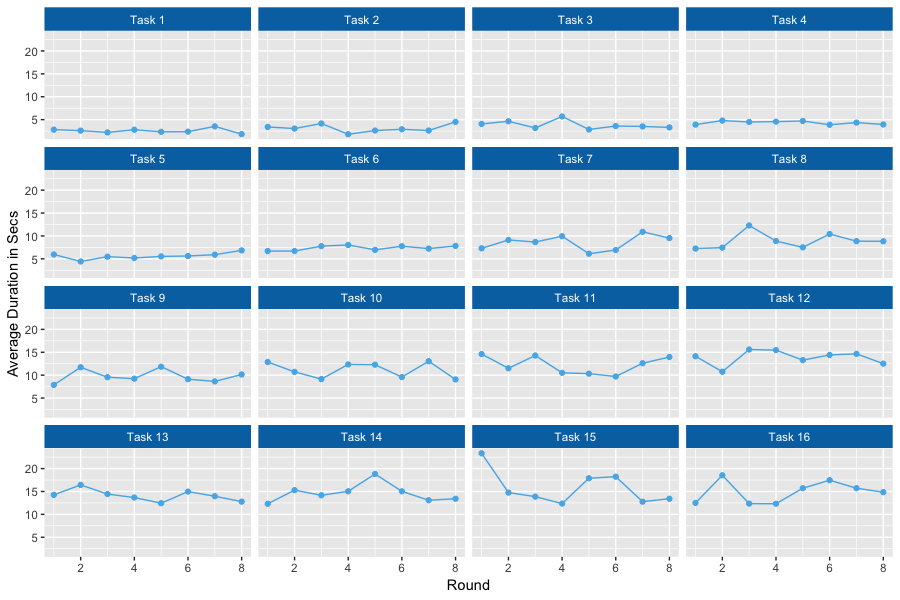
\includegraphics[width = \textwidth]{graphs/avg_time_per_task_round.png}
        \caption{Average time in seconds needed to solve the first 16 tasks across rounds}
        \label{fig:avg_time_task}
    \end{figure}
    
    
    \subsection{Benchmarking}
    \label{ss:benchmarking}
    
    To identify the levels of performance outside competition, two rounds of the RET are played during the introductory section of the experiment. In the first round, participants receive what will be the low piece rate (the payment per sequence if they do not win the contest), while in the second they receive the high piece rate (the payment per sequence if they are declared the winner of a period). The latter piece rate was, in my case, double the low piece rate such that a participant would take up to twenty seconds solving a sequence before switching to the leisure mode. The order of the benchmark rounds, first low, then high piece rate, was selected to make the difference in earnings between them more salient.
    
    Instructions and control questions were shown before the low and high piece rate paying benchmarking rounds. In the control questions before the high wage benchmark, I chose the possible answers such that selecting the correct answer for the low wage benchmark round would be possible, so forcing participants to think why there was a change in the maximizing time to solve sequences. Participants could only advance if they responded all control questions correctly.
    
    \subsection{Feedback}
    
    During solving of the RET a summarized version of the instructions is shown at the bottom of the page and a mouseover display explains all relevant elements if needed. Once a participant goes into the \textit{switch} mode, a counter shows live how many tokens he or she earns with each passing second and informs him or her about the number of sequences solved.\\
    
    Finally, a feedback screen shows how many sequences were solved, how much time spent in the \textit{switch} mode and how many the total earnings for the round are. In the second round of the baseline setting RET, another table informs the participant about the earnings of the previous round to make the difference in earnings, between the high and the low piece rate, more salient. \textcolor{red}{A selection of screenshots is provided in the Appendix}
    
    \section{Introductory Section}
    \label{sec:intro_exp}
    
    The introductory section welcomes the participants and instructs them into the functioning of the experiment and the Real Effort Task (RET).
    
    \subsection{Real Effort Task Instructions and Trial Round}
    
    After a short introduction to the experiment, participants are explained the main goal of the RET (counting ``a''s) and how the submission works (typing the correct number in the input field and hitting ``enter''. See section \ref{sec:RET} for more detail). They then have the opportunity to test the task five times with five different sequences that were chosen to show the variability of the sequences. Some were long and some were short, some had many and some had few ``a''s. When a correct answer is submitted, the next sequence is shown and the current timer is restarted. \\
    
    The screen also featured an annotated tour that explained every part of the RET screen: the sequence, the input field, and a timer counting the number of seconds needed to solve the current and the previous sequence. \textcolor{red}{A screenshot is provided in the appendix.}\\
    
    \subsection{Switch Mode Instructions}
    
    After participants have completed the trial round, they are introduced to the leisure mode, the payment scheme, and the increasing difficulty mechanism of the RET. The incentivised leisure mode is a core feature of my experiment and it is explained in more detail in section \ref{sec:RET}. During the experiment it is called \textit{switch} mode to avoid any stigma on shirking.\\
    
    Participants are paid one token per correctly solved sequence with one token being converted to EUR 0.1 at the end of the session. While in the ``switch'' mode, they earn 0.1 tokens per each second spent in it. Great effort is put in this screen to let participants know that, given the payoffs, the ideal point to switch is when he or she takes longer than 10 seconds to solve a sequence, regardless of how much time is left or how many sequences they have solved thus far. However, I do not explicitly write that as the optimum since in the competition rounds it might be advisable to solve more sequences to increase the chances of a higher piece-rate.\\
    
    In this screen, an illustrative example of possible earnings is presented, participants can test the RET several times, and an annotated tour introduces the new elements (a counter of total solved sequences a timeout, and the switch button).
    
    \subsection{Control Questions}
    
    In this page, participants are asked two sets of questions to ensure that they have understood the instructions. To be able to proceed, they have to answer all questions correctly.\\
    
    In the first set, participants are asked how much a fictional player would have earned given an amount of solved sequences and time spent in the \textit{switch} mode (fig. \ref{fig:cq_earnings}). The numbers were chosen so they would not offer an obvious anchor point\footnote{An anchor point being an amount of time or sequences solved that a participant is supposed to aim to while solving the RET} while still being easy to calculate.\\
    
    \begin{figure}
        \centering
        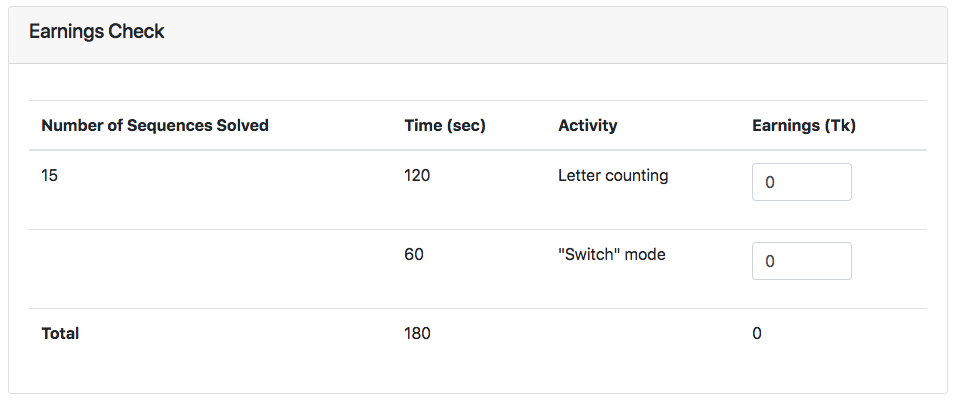
\includegraphics[width=\textwidth]{graphs/cq_earnings.png}
        \caption{Control Question Earnings}
        \label{fig:cq_earnings}
    \end{figure}
    
    In the second set (fig. \ref{fig:cq_switch}) participants were asked to select the switching point of a fictional player aiming at maximizing her payoff. Also here the times were selected in such a form, that a tendency to infer an anchoring point would be minimized. Similarly, instead of giving examples of actual sequences, only a visualization with bars is given.
    
    \begin{figure}
        \centering
        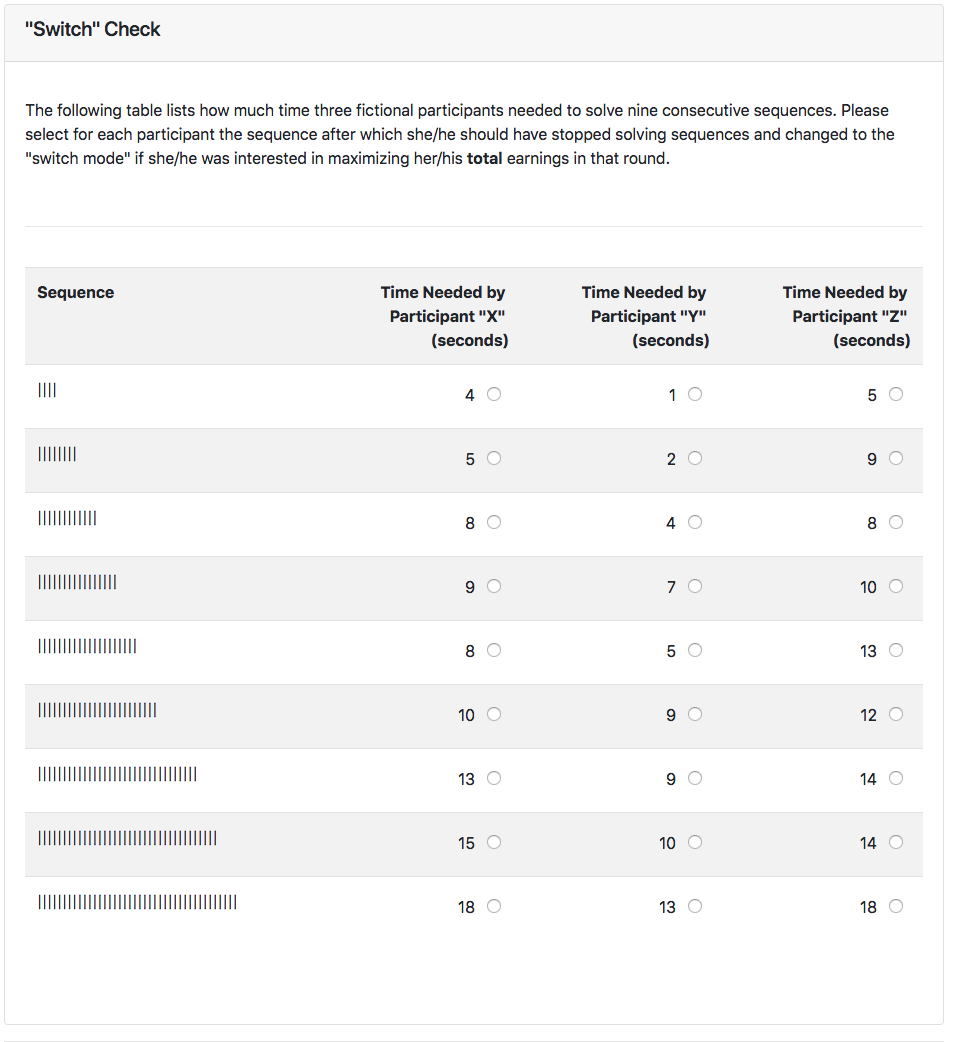
\includegraphics[width=\textwidth]{graphs/cq_switch.png}
        \caption{Control Question ``Switch'' Mode}
        \label{fig:cq_switch}
    \end{figure}
    
    
    \section{Competition Section}
    \label{ss:compt}
    
    At the beginning of the competition section, participants are informed that they were selected randomly into groups of three people and that each person was assigned a label \textit{A, B} or \textit{C}, but that their identity and that of all other participants will remain anonymous both to all other participants as well as to the experimenters\footnote{in order to reduce the impact of other-regarding behavior}. \textcolor{red}{Expand: I choose three participants since it allows for a more dynamic setting, without increasing complexity too much. It is possible, for instance to differentiate between last place and second place.}  Participants in the treatment sessions are further informed at this stage about the taxation and redistribution scheme (see section \ref{sec:treat}).\footnote{ Note that when moving from the introductory section to the competition, two things change in regard to the RET and the performance incentives. First, the competitive aspect of being in the group. Participants will have the possibility to see what others do and will know, that the other participants will see their own performance. In fact, last place aversion and the utility of winning itself have been shown to be the driving issues behind overbidding in rent-seeking contests as well as behind performance increase in competitive games \citep{sheremeta2013}. Second, the actual contest where increasing one's earnings can also indirectly increase the chances of winning the prize trough a larger available income to invest.\\
    The fact that those two factors change at once might difficult pin-pointing reasons for a performance change between the benchmarking and the competition rounds. This does, however, not affect any of the main variables I am interested in in this study since we can still precisely determine the optimal investment and switching time for each participant and the difference to the observed measures. Furthermore, the effect of competition, inequality, impulsivenes, etc. have already been extensively researched, including in the context of rent-seeking contests. In fact, \cite{sheremeta2016} shows that the main factor is impulsiveness which I control for as explained in subsection \ref{ss:CRT}. For those reasons, I leave the experiment as is, but discuss a possible workaround and its drawbacks in chapter \ref{ch:discussion}.} 
    
    \subsection{Tullock Contest}
    
    Next, players are informed  about the contest proper. In eight rounds, each participant will have the opportunity to earn money by solving the letter counting task or spending time in the ``switch'' mode. Money earned trough work \footnote{the net income from counting letters plus the redistributed amount} can then be invested to increase the higher piece rate in the following round. Only one person per round is awarded the prize and the probability of winning it is equal to the share of that person's investment relative to all investments by all players. An example for easier understanding is also shown.\\
    
    Players are further reminded at this stage of how much they earned in the benchmarking rounds and of the difference in earnings between the low and high piece rate rounds.
    
    \subsection{Beliefs}
    
    To test if and to what extent players take into account the behavior of the others when choosing their production and investment levels, beliefs about the production, i.e. the number of sequences solved, and the amount invested by the other team members are elicited in every round. A visual clue lets them know which player has a higher piece rate in the current round.
    
    \subsection{Feedback and Result}
    
    After solving the task and before investing, as in the introductory section, participants receive feedback on their performance: how many sequences were solved, how many seconds spent in ``switch'' and, in the case of the treatment, how much the transfers are.\\
    
    After the investment, participants become detailed feedback about the investments and performance of the group and are informed of who won the high piece rate in the following round (see fig. \ref{fig:screen_results}).
    
    \begin{figure}
        \centering
        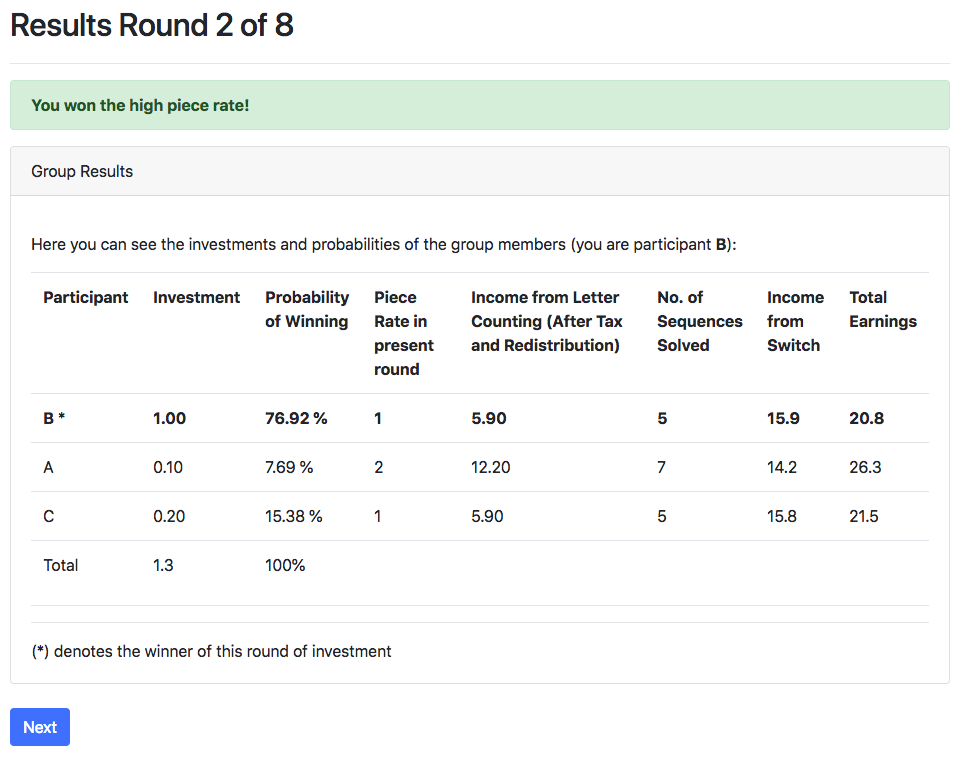
\includegraphics[width=\textwidth]{graphs/screen_results.png}
        \caption{Results Screen after Investment}
        \label{fig:screen_results}
    \end{figure}
    
    \subsection{Investment}
    
    On the investment screen, players use a slider to choose their investment in steps of 0.1 tokens. They are informed about their total available income for investment, how much they invest, how much they would keep and what the prize is. They are also reminded that tokens invested are not refunded, even if the prize is not awarded (see fig. \ref{fig:screen_invest}).
    
    \begin{figure}
        \centering
        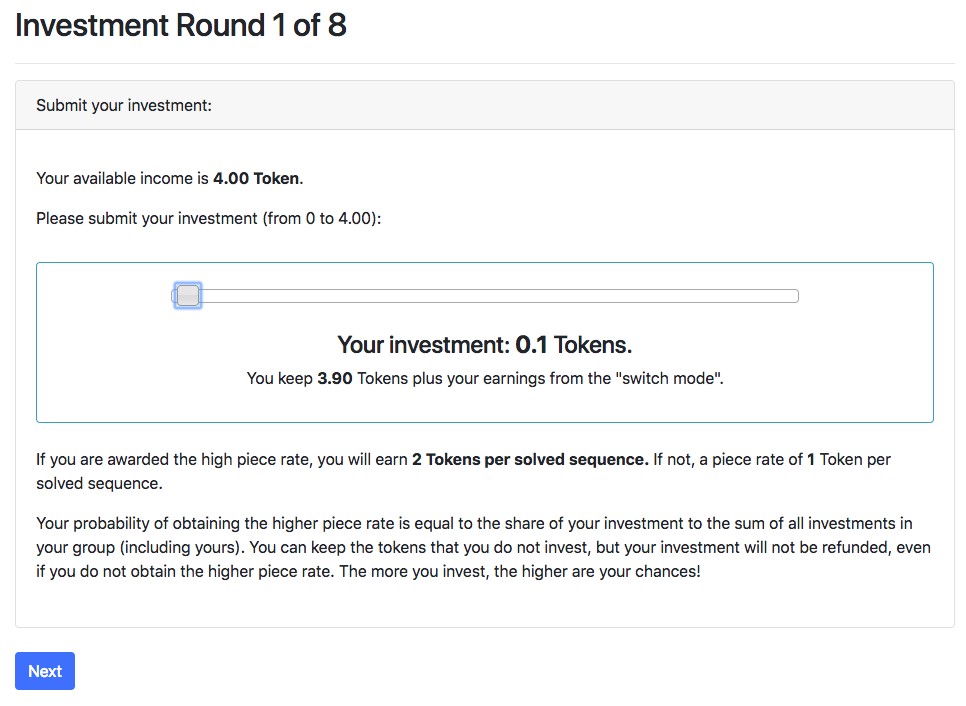
\includegraphics[width=\textwidth]{graphs/screen_invest.png}
        \caption{Investment Screen}
        \label{fig:screen_invest}
    \end{figure}
    
    
    \section{Treatment: Taxation and Redistribution of Income}
    \label{sec:treat}
    
    As explained in this Thesis introduction, understanding how voting would affect the POUM itself requires several layers of examination. In the present work, I have a look at how the general dynamics of the contest behave and which impact taxation and redistribution have on the distribution of win probabilities and the exertion of effort.\\
    
    To test this, I introduced a treatment where income from work, that is, from counting letters, is taxed at 60\%. The entire tax revenue is then divided equally among all participants so that the total amount of tokens in circulation is constant. Participants can then invest their net income plus transfer to increase their chances to earn the higher piece rate as explained in section \ref{ss:compt}.\\
    
    In the control group there is no taxation and therefore no redistribution. The available income to invest is exactly equal to the earned tokens from letter counting. Note that the predictions regarding the optimal investment as derived in chapter \ref{ch:model} are unchanged since taxation and redistribution only affects work income. However, taxation does affect the valuation of the game where $\mathbb{V}$ is no longer equal to just the difference in earnings between the high and low wages, but adds the share of the sum of redistributed income $R$ such that $\mathbb{V}_i = x_{hw}*w_{hw} - x_{lw}*w_{lw} + \frac{R}{n}$\footnote{where x is the amount of sequences solved, $w$ the paid piece rate, and $hw$ demarks the high and $lw$ the low wages}.\textcolor{red}{prepare for the question of how this affects \ref{eq:exp_util}: it doesn't we take valuation as given and known to each participant. \ref{eq:exp_util} only takes into account the investment amount. Further, we assume equality among participants which means it doesn't matter who is at the top to determine redistribution}  
    
    \subsection{Taxed Benchmarking}
    \label{ss:tax_bench}
    
    To better measure the valuation of the price in the taxation treatment, two extra rounds paying a wage equal to the effective taxation in the treatment were added to the benchmarking phase for the treated group as explained in subsection \ref{ss:benchmarking}.\\
    
    Specifically, in between the low piece rate and high piece rate benchmarking another benchmark round was introduced. This round payed per task the equivalent of the effective taxed low piece rate after redistribution or $w(1-t)+ w(t/n)$\footnote{If the total tax revenue is divided in equal parts among all individuals, as is the case in my design.}, with $w$ being the piece rate, $t$ the tax rate and $n$ the number of players per group. In my case this means 0.6 tokens per sequence or 1 token minus 40\% of 1. The payment for the \textit{switch} mode remained, as in all rounds, constant.\\
    
    Similarly, an extra round was introduced after the high wage round which payed the equivalent of the effective taxed high piece rate after redistribution, in our case, 1.2 tokens or 2 tokens minus 40\% of 2. These extra rounds were introduced in this order so as not to generate a strong separation between the taxed and the untaxed rounds, as well as to space out the control questions. \\ 
    
    To control that introducing these extra rounds did not affect participants' performance, I carried out a Wilcoxon test between the productions of the treated and non treated groups. Once for the low benchmark and once for the high piece rate benchmarking rounds. Both showed no differences between groups, i.e., no learning or timing effects, nor a significant difference in skill. The test results are summarised in the appendix in table \ref{tab:bench_prods_test}.
    
    \section{Idiosyncratic Controls}
    
    To control for the effect of idiosyncrasies, like risk aversion, on players' behavior, I introduced several tests at the end of the experiment which are presented in this section. 
    
    \subsection{Fairness Sentiment}
    
    To see how participants themselves perceived the game in terms of what determined success, they were asked to rate from 0 to 7 what determined their success in the game. With 0 being only luck and 7 being only skill. Image \ref{fig:fair_q} shows the voting screen. The question was posed both at the beginning and end of the competition. Allowing us to observe not only how the perception changes after experiencing the competition, but if and to what extent the fairness perception changes in the presence of redistribution.\\
    
    This measure can furthermore be useful in comparisons with other designs and parametrizations as discussed in the discussion in chapter \ref{ch:discussion}.
    
    \begin{figure}
        \centering
        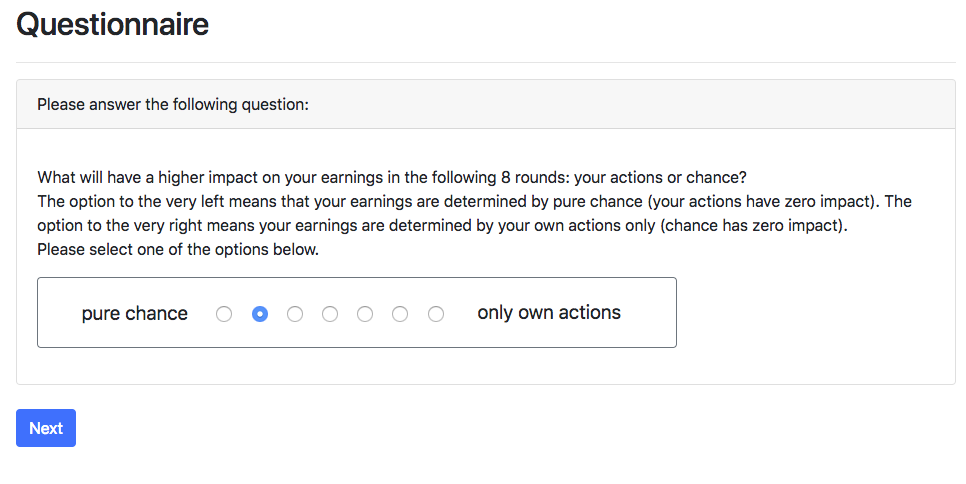
\includegraphics[width=\textwidth]{graphs/Fairness_Q_Begin.png}
        \caption{Screen Fairness Questionnaire (beginning)}
        \label{fig:fair_q}
    \end{figure}
    
        
    \subsection{Risk Aversion Measure and Risk Elicitation}
    
    During the investment section of the experiment players participate, effectively, in a lottery. The exact terms of that lottery are not known to them in advance and present an strategic decision as well. Their investment choices will therefore not only reflect their strategic considerations, but also their stance on risk taking.\\
    
    To control for this I include an incentivised risk elicitation test following the \textit{Multiple Price List} by \cite{holt2002} (HL) with the implementation for \textit{oTree} taken from \cite{holzmeister2017}.\\
    
    I chose the HL method as it, according to \cite{crosetto2016} and \cite{harrison2008}, among other things:
    \begin{itemize}
        \item allows for risk preferences in both the risk neutral and risk seeking range
        \item has a finer categorisation as for instance \cite{eckel2008}
        \item has constant intervals between the parameters of risked mapped trough choices which makes it robust to stochastic decisions
        \item there are no significant differences between genders
    \end{itemize}  
       
     In the HL method, players are asked to choose between several pairs of lotteries, A and B. Beginning with a choice where option A is the safer choice, the last choice is between sure outcomes, where B represents the payoff maximizing choice. Between them, there is a point where a participant changes from one option to the other, thus revealing her risk preferences.\\
     
     Figure \ref{fig:choices_mpl} shows the list of choices that participants were presented with. In it, probabilities are visualized with the help of pie charts and all possible decisions are shown at once. Consistent preferences were forced to avoid elimination of data in the already small sample. After choosing, one of the decisions was then selected randomly and the lottery drawn and paid out.\\
     
     \begin{figure}
         \centering
         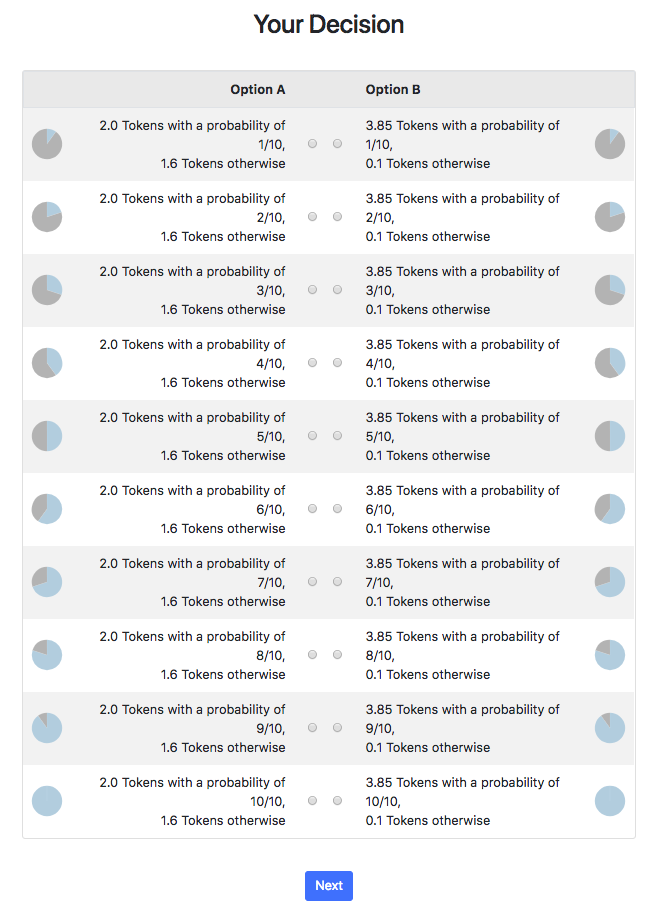
\includegraphics[width=\textwidth]{graphs/Choices_MPL.png}
         \caption{Choices Screen \textit{Multiple Price List}}
         \label{fig:choices_mpl}
     \end{figure}
     
     
    Following the common procedure I assume participants to have a constant relative risk aversion (CRRA) utility function $u(x)=x^{(1-r)}$, which allows to index each choice by a corresponding $r$. An individual with an $r<0$ is categorized as risk averse, with $r=0$ as risk neutral and with $r>1$ as risk seeking. The payoffs are exactly equivalent to those used by \cite{holt2002} and thus imply, that someone switching after the fourth lottery to \textit{option B} is assigned an $r$ interval of (-0.15, 0.15) meaning risk neutrality. The list of the implied risk aversion ranges can be seen on table \ref{table:HL} where the number of safe choices is the number of choices before switching to \textit{option B}.
    
    
    \begin{table}[]
    \centering
    \begin{tabular}{lll}
    \hline
    \hline
    \begin{tabular}[c]{@{}l@{}}Number of \\ Safe Choices\end{tabular} & \begin{tabular}[c]{@{}l@{}}Range of Relative\\ Risk Aversion\end{tabular} & \begin{tabular}[c]{@{}l@{}}Risk Preference \\ Classification\end{tabular} \\
    \hline
    0-1                                                               & r < -0.95                                                                 & Highly Risk Loving                                                        \\
    2                                                                 & -0.95 < r < -0.49                                                         & Very Risk Loving                                                          \\
    3                                                                 & -0.49 < r < -0.15                                                         & Risk Loving                                                               \\
    4                                                                 & -0.15 < r < 0.15                                                          & Risk Neutral                                                              \\
    5                                                                 & 0.15 < r < 0.41                                                           & Slightly Risk Averse                                                      \\
    6                                                                 & 0.41 < r < 0.68                                                           & Risk Averse                                                               \\
    7                                                                 & 0.41 < r < 0.97                                                           & Very Risk Averse                                                          \\
    8                                                                 & 0.41 < r < 1.37                                                           & Highly Risk Averse                                                        \\
    9-10                                                              & 1.37 < r                                                                  & Stay in Bed\\
    \hline
    \end{tabular}
    \caption{Risk Aversion Classifications Based on Lottery Choices\\ \citep{holt2002}}
    \label{table:HL}
    \end{table}
    
    \subsection{Cognitive Reflection Test}
    \label{ss:CRT}
    
    A tendency to overbidding in rent-seeking contest has been well documented \citep{sheremeta2013, dechenaux2015}. This is particularly critical in my design as overbidding, both in terms of work supply and investment, would be interpreted as an over-exertion of effort.\\
     
    While there are several proposals as to what influences this behavior, \cite{sheremeta2016} suggests that impulsiveness might be the strongest predictor. In fact, he suggests that when analyzed simultaneously with the utility of winning, systematic biases, relative payoff maximization, and mistakes, only impulsiveness remain statistically significant.\\
    
    Following him I therefore include a \textit{Cognitive Reflection Test} based on \cite{thomson2016}. The latter propose alternative questions that also measure cognitive reflection but are less well known. Figure \ref{fig:crt_quest} shows the questions that participants were presented. although they were presented singularly and without the possibility to go back, instead of all at once.
    
    \begin{figure}
        \centering
        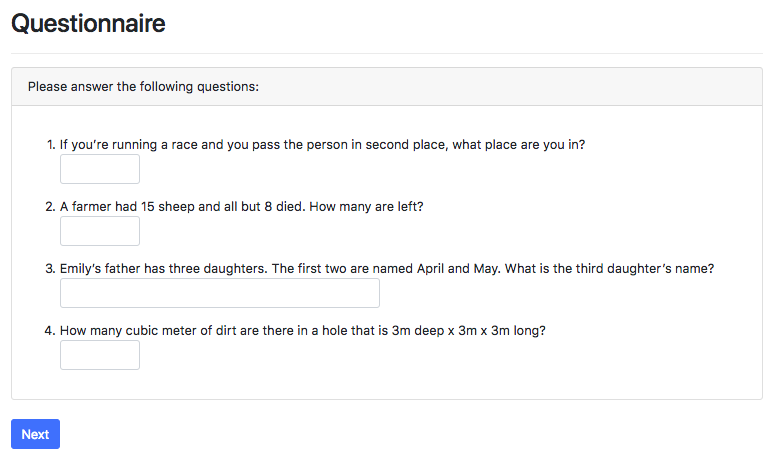
\includegraphics[width=\textwidth]{graphs/CRT_Quest.png}
        \caption{Cognitive Reflection Test \citep{thomson2016}}
        \label{fig:crt_quest}
    \end{figure}
    
    \section{Hypotheses}\label{sec:hyp}
    
    I focus in this thesis on the dynamic of repeated Tullock Contests, in particular regarding the tendencies of participants to over-invest, and the evolution of winning probabilities across periods. As explained in the introduction, those probabilities can be seen as analogous to the Prospect of Upward Mobility while the investments made in each round are analogous to investments made in human capital needed to acquire high earning jobs.\\
    
    Broadly speaking, my thesis has a look at performance values in terms of sequences solved and time spent in leisure mode, and at effort exertion values in form of investments. Comparisons in those regards are made both within and between subjects and groups. Within subjects and groups I will look at the differences between the benchmark and the competitive rounds in general, and within the competition rounds across time. In addition, I introduce a taxation and redistribution intervention which will be studied through a between-subject and group comparison.\\
    
    How investments develop across periods is the first step to analyze the POUM in my experiment. How much participants invest ultimately determines the probabilities of winning, but more importantly, it determines the total welfare of the group. Since available income invested is not reimbursed, investments reduce overall welfare. An intervention that reduces over-investment while ensuring fairer\footnote{The definition and analysis of the concept of fairness go far beyond the scope of the present thesis but are addressed in chapter \ref{ch:conclusion} as part of the discussion.} winning probabilities is therefore desirable.\\
    
    As described in the model in chapter \ref{ch:model}, investments should be constant over time, however, as \cite{sheremeta2016}, among others, have shown, participants tend to over-invest. I expect, nevertheless, that over-investment decreases over time, due to income effects or to better knowledge of the game. This phenomena is shown experimentally by \cite{fallucchi2013} where, although investment levels stay above optimum, they clearly drop in the presence of full information  as it is the case in my design. In that experiment, groups with full information reduced over-investment to around 13\% above optimum while those with only feedback about their own performance stayed at levels of 66\% above optimum. Formally, I expect therefore that:
    
     \begin{hyp} \label{hyp:treat}\textit{Mean investments will be higher than the expected profit maximizing value for all treatments, but decreasing over time.}\end{hyp}
    \hfill\newline 
    As it has been described in the literature of rent seeking contests, over-investment can be driven by several aspects, most importantly, impulsiveness, risk incline, competitiveness and inequality aversion. When introducing a redistribution scheme specially the latter characteristic might be affected as income distributions within groups become more equal. Given the fact that the available income is more equally distributed in the treatment by design, if inequality aversion plays a role, I expect investments in the taxed groups to be relatively lower. Formally:
    
    \begin{hyp} \label{hyp:treat-overinvest}
    \textit{Participants in the treatment will invest a lower share of their optimal investment}
    \end{hyp}
    
    In other words, participants in the treatment will be relatively closer to their optimal investments. Note that the compared measure is the ratio over the optimum since the optimal value of investment is different for both groups. This is because the valuation of the game, i.e. the difference in net earnings between the high and the low wage, is different for each treatment.\\ 
    
    I control for risk aversion and impulsiveness with the methods mentioned above in the experimental design section (\textit{Cognitive Reflection Test} and \textit{Multiple Price Listing}). Furthermore, if competitiveness plays a major role I should observe no major difference between treatments or across time. What leads to the second part of hypothesis \ref{hyp:treat}: not only do I expect investments to be higher than optimal but to be decreasing over time. If that decrease is driven mainly by a better understanding of the game or better knowledge of other participant's behaviour, I should not observe any difference in slope between treatments. In the latter case I would further expect an increase in the accuracy of a participant's belief over the investment AND performance (since performance determines the valuation) of the group's other participants.\\
    
    On the other hand, the reduction in investments effect can be driven by an income effect, since in each period only one person wins but two lose. If winners of previous rounds are more likely to invest more and therefore also more likely to win again, losers might invest less each time.  In this case, I should observe a significant difference between winners and losers and a significant effect of cumulative wins on the invested amount.\\
    
    A third possibility is that participants have a decreasing utility function for winning. In other words, that participants value winning the first round higher than winning the last one. My design does not allow to disentangle this effect from experience effects but the issue is discussed for further research in chapter \ref{ch:conclusion}.\\
      
    An important corollary of \cref{hyp:treat} is that, since players are closer to the optimum levels of investment, total welfare for the group in terms of total income generated is larger.\\
    
    Now, what does the expected lower over-investment for the treatment and the decreasing investments over time mean for the probability of winning? In other words, how do investments change relatively to the other group members in the cross-sectional and longitudinal dimensions?\\
    
    If investments decrease over time mainly due to subject specific differences (learning, decreasing utility of winning, etc.) I should not observe any significant differences between treatments or across time regarding the distribution of probabilities. If, however, the effect is driven by group dynamics, for instance last place aversion or income effects of cumulative wins I expect to see a stronger variance in probabilities in the control while increasing over time. In the redistribution treatment, available income will be more equally distributed and therefore inequality and income effects should be diminished. In other words, probabilities will be closer to each other and to the mean of $1/n$. Formally:
    
    \begin{hyp}\label{hyp:wins}
    \textit{The coefficient of variance of winning probabilities will be increasing across rounds while being smaller in the treatment.}
    \end{hyp}
    
 
\chapter{Results}
\label{ch:results}
\thispagestyle{fancy}

The participants of the experiment were selected on a first come, first served basis from registered volunteers of the \textit{Vienna Center for Experimental Economics} who spoke English, were under 40 years of age, and had not participated in more than 10 previous experiments. A total of 96 people (55 female and 41 male) with an average age of 25 years took part in a total of four sessions during the second half of 2018. Two of the sessions ran the control while the others two ran the treatment, such that exactly half the participants were in the treatment and half in the control.\\

At the end of the session, participants were paid anonymously, in private, and in cash, ranging from EUR 12.50 to 31.30 for an average payoff of EUR 22.90.\\  %\textcolor{red}{\textbf{To be discussed}: All data, scripts and results are available at XXX.XXX.XXX, even those that for space reasons were not included in the print version of this thesis.}

All the data preparation, analysis and visualization for this thesis was done using the statistical software \textit{R} \citep{rcoreteam2014}.\footnote{Packages used: \textit{tidyverse} \citep{wickham2017b}, \textit{data.table} \citep{dowle2018}, \textit{ineq} \citep{zeileis2014}, \textit{stargazer} \citep{hlavac2018}, \textit{ggplot2} \citep{wickham2016}, \textit{sjstats} \citep{ludecke2018}, \textit{texreg} \citep{leifeld2013}, \textit{ggthemes} \citep{arnold2018}, \textit{ggridges} \citep{wilke2018}, and others which are referenced in due course.} 

\section{Notes on the Methodology}

Although ANOVA models are commonly used in behavioral sciences when analyzing treatment differences in repeated measures, several authors have questioned their adequacy (\cite{camilli1987}, \cite{vasey1987}, \cite{jaeger2008}, \cite{locker2007}, \cite{krueger2004}). Especially critical in my design is the fact that participants are matched in groups which do not change during the experiment and may therefore develop their own dynamic. Imagine, for instance, a group in which the majority of participants are very risk friendly or have a high valuation. Investments might increase in total, even for those participants that are not as risk loving.\\ 
    
Instead, linear mixed models as used, for instance, by \cite{szaszi2018}, \cite{holsen2009} or \cite{yue2010}, are encouraged since they allow the study of the general effect of the variables of interest while allowing random intercepts for groups and participants and also whilst taking the auto-correlation of the repeated measure into account (\cite{galecki2013}, \cite{bolker2009}, \cite{mcculloch2015}, \cite{barr2013}, \cite{baayen2008}, \cite{fitzmaurice2015}). I therefore generally use a linear mixed model specification to be compared against a "fixed effects only" model in the results analysis below.\\ 
%Not included since there is no explicit model selection
%If not indicated otherwise, I chose the model by minimizing Akaike's Information Criterion which penalizes both a too simple and a too complex model.\\

\section{Preliminary Results}

Before diving into the hypotheses regarding investment and winning probabilities as postulated in section \ref{sec:hyp}, we want to get a sense of the general behavior patterns participants exhibited during the competition, particularly regarding the solution of the RET and how that behavior differed between treatments.

\subsection{Task Solving}
\label{sec:seq_prod}

During the benchmarking rounds, participants solved around 10 sequences and were paid one token per sequence. With the high piece rate of two tokens per sequence, participants solved an average of 15.3 sequences. The mean valuation, that is, the mean difference between the earnings (income from solving sequences plus income from the leisure mode) in the low and the high piece rate was of around 13 tokens. Table \ref{tab:avg_prod_bench} summarises these findings.

\begin{table}[!htbp] \centering 
  \caption{Mean Values of Production in Benchmark} 
  \label{tab:avg_prod_bench} 
\begin{tabular}{@{\extracolsep{5pt}} cccc} 
\\[-1.8ex]\hline 
\hline \\[-1.8ex] 
 & \makecell{avg. prod. \\ low wage (seqs)} & 
 \makecell{avg. prod. \\ high wage (seqs)} & mean valuation (tks)\\ 
\hline \\[-1.8ex] 
control & 9.77 & 15.29 & 12.9 \\ 
treatment & 10.25 & 15.29 & 13.09 \\ 
\hline \\[-1.8ex] 
\end{tabular} 
\end{table} 

During the competition, participants solved an average of 11.5 sequences and spent an average of 85.2 seconds in the ``switch'' mode. There was little difference in production between wages, i.e. between winners and losers, but some difference can be observed between treatments. Subjects in the treatment produced less on average and spent more time in the ``switch'' mode. Table \ref{tab:avg_prod} and Figure \ref{fig:production_boxplot} summarize these findings.\\

\begin{table}[!htbp] \centering
  \caption{Mean Values of Production\\
    \footnotesize{standard errors are reported in parentheses ()}} 
  \label{tab:avg_prod}
\begin{tabular}{@{\extracolsep{5pt}} cccc} 
\\[-1.8ex]\hline 
\hline \\[-1.8ex] 
 & wage & mean of solved sequences & mean of time spent in ``switch'' \\ 
\hline \\[-1.8ex] 
control & 1 & 12.02 & 78.66 \\ 
 &  & (0.23) & (3.13) \\ 
control & 2 & 11.91 & 79.09 \\
 &  & (0.3) & (4.22) \\ 
treatment & 1 & 11.1 & 92.28 \\
 &  & (0.21) & (2.86) \\ 
treatment & 2 & 11.12 & 90.23 \\
 &  & (0.33) & (4.42) \\ 
\hline \\[-1.8ex]
\end{tabular}
\end{table}  

\begin{figure}
    \centering
    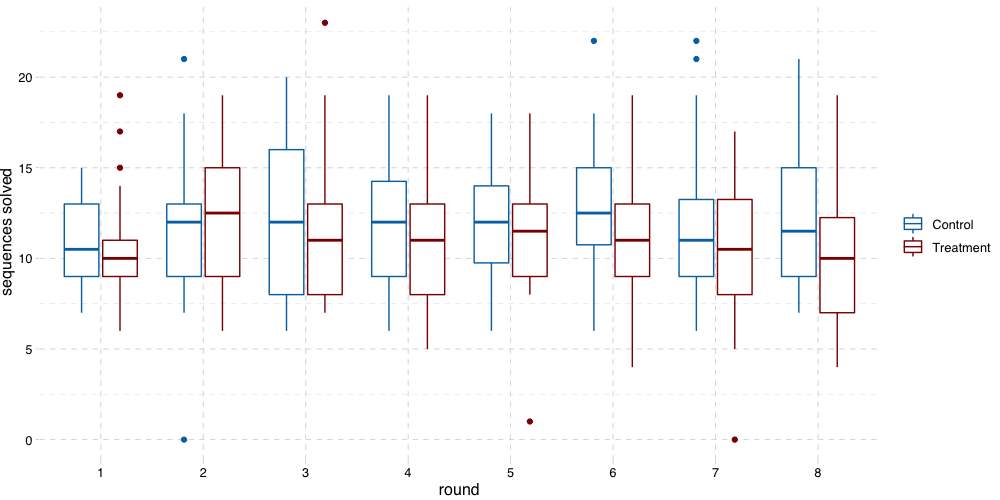
\includegraphics[width=\textwidth]{graphs/production_boxplot.png}
    \caption{Number of Sequences Solved per Round and Treatment}
    \label{fig:production_boxplot}
\end{figure}
    
To see if the difference in production between the treatments is statistically significant, and to see how other factors play a role, I used a linear mixed model (LMM) with random intercepts evaluated using the \textit{R} package \textit{lme4} \citep{bates2015}. Since the design only allows for between-group comparisons in the treatment, I do not include a random slope per participant, assuming thus that the effect of time will be the same for all subjects.\\

In this model, the fixed effects are: the \textit{treatment}, \textit{was winner} (if a participant won the previous round and is playing with the high wage), and the \textit{round} number. The random effect is the \textit{subjects id} nested within the \textit{group}. Results are largely reported following \cite{barr2013} and are summarized in Table \ref{table:lmer_prod} in the \textit{sequence production} column. P-values were calculated using the likelihood ratio test of the \textit{R} package \textit{lmerTest} \citep{kuznetsova2017}.\\

\textit{Treatment} has a small effect, though significant at the 10\% level, with subjects in the control group solving just shy of 1 sequence more per round (+0.872). All the other fixed effects have no significant or large effect with the model in total explaining 42\% of the observed variance in which the fixed effects explain 1.52\% (conditional R-squared and marginal R-squared respectively, calculated using the \textit{psycho} package \citep{makowski2018}). The variables with no effect include, interestingly, the wage at which participants played.\\

%Not included since Loy argues not necessary
%Note that although the residual plot and QQ-plot do not make apparent any deviation from a normal distribution nor any systematic increase or decrease in variance, there is much debate as to how to appropriately check for the validity of assumptions in LMMs  \citep{loy2017}, specially when dealing with distributions other than normal, and will therefore not be addressed here in this thesis.\\

It is important to remember that in this experimental design, payoffs are not exclusively determined by the amount of sequences solved. They depend also on: the time spent in the ``switch'' mode and therefore on the optimal change to it, the invested amount in human capital, and, in the treatment, how much the other players worked. The boxplot in Figure \ref{fig:earnings_boxplot} seems to suggest that the net income is higher in the treatment groups and that, apart from the transition from round 1 to round 2, it does not change over time. Note that, here, net income describes income after taxation \textit{and} redistribution, but before investment. The variance of the treatment is smaller since, in that group, by definition, net incomes are closer to each other.\\

In order to see if there were significant differences in net income between treatments, I use a model with fixed effects (\textit{treatment, was winner} and \textit{round}) and summarise the findings in the \textit{net income} column of Table \ref{table:lmer_prod}.\\

\begin{table}[!htbp] \centering 
  \caption{Linear Mixed Model - Sequence Production and Net Income} 
  \label{table:lmer_prod} 
  \scalebox{0.8}{%
\begin{tabular}{@{\extracolsep{5pt}}lcc} 
\\[-1.8ex]\hline 
\hline \\[-1.8ex] 
 & \multicolumn{2}{c}{\textit{Dependent Variable:}}\\ 
\cline{2-3} 
\\[-1.8ex] & Sequence Production & Net Income \\ 
\hline \\[-1.8ex] 
 treatment & $-$0.872$^{*}$ & 0.598 \\ 
  & (0.499) & (0.471)\\ 
  & \\ 
 was winner & 0.028 & 5.977$^{***}$\\ 
  & (0.231) & (0.289)\\ 
  & \\ 
 round & $-$0.003 & 0.090$^{*}$\\ 
  & (0.043) & (0.054) \\ 
  & \\ 
 Constant & 11.985$^{***}$ & 21.434$^{***}$\\ 
  & (0.408) & (0.422)\\ 
  & &\\ 
\hline \\[-1.8ex] 
Observations & 768 & 768 \\ 
Log Likelihood & $-$1,943.528 & $-2,098.867$\\ 
Akaike Inf. Crit. & 3,901.055 & $4,211.735$\\ 
Bayesian Inf. Crit. & 3,933.525 & $4,244.241$\\
\hline \\ [-1.8ex] 
Var: participant|group (Intercept) & 5.08 & 3.86\\
Var: group (Intercept) & 0.00 & 0.00\\
Var: Residual & 7.28 & 11.77\\
\hline \\[-1.8ex] 
\hline 
\textit{Note:}  & &\multicolumn{1}{r}{$^{*}$p$<$0.1; $^{**}$p$<$0.05; $^{***}$p$<$0.01} \\ 
\end{tabular}
}
\end{table} 

Winning the previous round, i.e. playing with the high wage has a strong and significant effect on net income while time, although marginally significant, has only a small effect. The introduction of a tax and redistribution scheme, on the other hand, does not have a significant effect. The model helps explaining 50.11\% (restricted R-squared) of the variance with the fixed effects accounting for 33.73\% (marginal R-squared) of the variance.\\

%Notice that while the taxation treatment has a negative impact on the number of sequences solved, it has no effect on net income. This is an indication that participants were over-performing in the control and, when confronted with a redistribution scheme, diminished their production such that the moment of switching to the leisure mode was closer to the optimum. Thus, they earned relatively equal, despite the effective tax rate of 40\%.\\

\begin{figure}
    \centering
    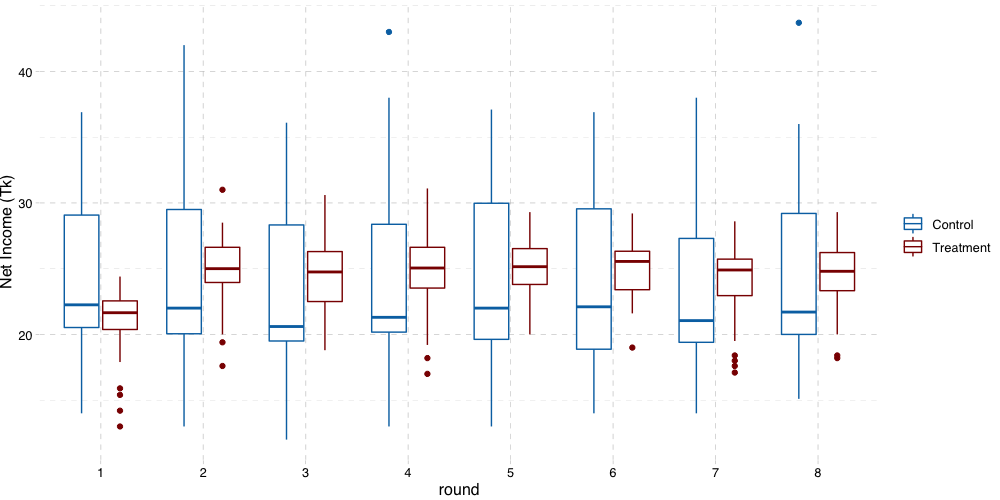
\includegraphics[width=\textwidth]{graphs/earnings_boxplot.png}
    \caption{Income after Taxation and Redistribution, and Before Investment}
    \label{fig:earnings_boxplot}
\end{figure}


%\begin{table}[!htbp] \centering 
%  \caption{Linear Mixed Model - Net Income} 
%  \label{table:earnings_lmer}
%  \scalebox{0.8}{%
%\begin{tabular}{@{\extracolsep{5pt}}lc} 
%\\[-1.8ex]\hline 
%\hline \\[-1.8ex] 
% & \multicolumn{1}{c}{\textit{Dependent variable:}} \\ 
%\cline{2-2} 
%\\[-1.8ex] & net income \\ 
%\hline \\[-1.8ex] 
% treatment & 0.598 \\ 
%  & (0.471) \\ 
%  & \\ 
% was winner & 5.977$^{***}$ \\ 
%  & (0.289) \\ 
%  & \\ 
% round & 0.090$^{*}$ \\ 
%  & (0.054) \\ 
%  & \\ 
% Constant & 21.434$^{***}$ \\ 
%  & (0.422) \\ 
%  & \\ 
%\hline \\[-1.8ex] 
%Observations & 768 \\ 
%Log Likelihood & $-$2,098.867 \\ 
%Akaike Inf. Crit. & 4,211.735 \\ 
%Bayesian Inf. Crit. & 4,244.241 \\ 
%\hline 
%Var: participant|group (Intercept) & 3.86          \\
%Var: group (Intercept)           & 0.00          \\
%Var: Residual                              & 11.77         \\
%\hline
%\hline \\[-1.8ex] 
%\textit{Note:}  & \multicolumn{1}{r}{$^{*}$p$<$0.1; $^{**}$p$<$0.05; $^{***}$p$<$0.01} \\ 
%\end{tabular}
%}
%\end{table} 


\subsection{Switching Time}
During the competition, participants appear willing to work more than their optimum in order to achieve a higher available income. Remember, participants should switch as soon as the time they need to solve a given task surpasses the earnings in the ``switch'' mode for the corresponding time. In the control group, players with the low wage should change as soon as they take longer than 10 seconds to solve the task and, in the treatment, as soon as they need more than six seconds. In each treatment, players with the high wage should switch at twice the respective time. Figure \ref{fig:time_per_task} shows the time needed for each task per round and marks the 10 and 20 seconds cut-offs.\\

It seems as if, in fact, the time needed to solve each sequence is more compressed to the middle in the control group. That is, fewer people are taking time above the cut-offs to solve sequences before switching. However, a Wilcoxon test\footnote{This is conducted using the \textit{stats} package \cite{rcoreteam2014}.} cannot reject the null hypothesis (p = 0 .283) of no shift with regard to the overall seconds over the 10 or 20 cut-offs. In chapter \ref{ch:discussion}, I address a design change that could make it easier to identify if there are general changes to the switching point when taxation is introduced.\\

\begin{figure}
    \centering
    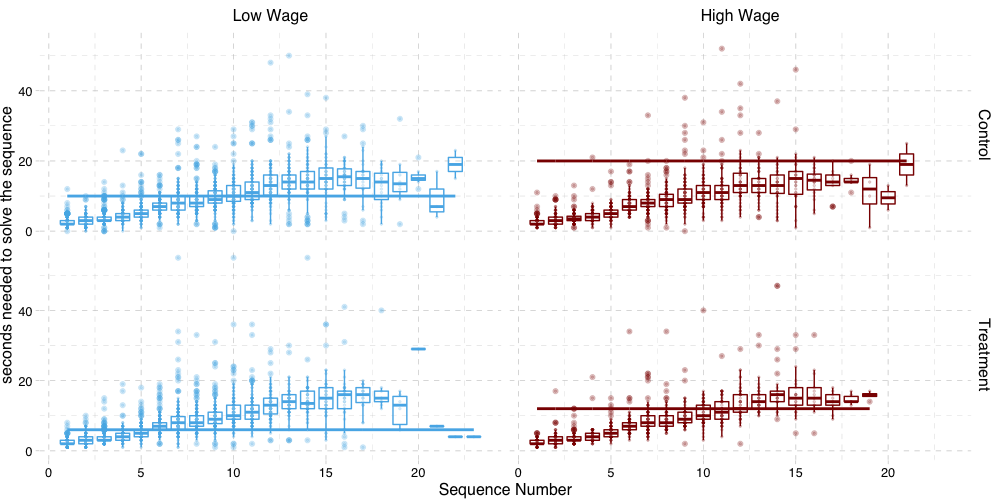
\includegraphics[width=\textwidth]{graphs/time_task_grid.png}
    \caption{Seconds Needed to Solve Sequences}
    \label{fig:time_per_task}
\end{figure}

\subsection{Controls}

In the \textit{Cognitive Reflection Test}, participants answered, out of a maximum of four, on average 2.22 (s.e. 0.1) questions correctly. Men answered, on average, 0.3 (s.e. 0.15) more questions correctly, with women giving 2.09 (s.e. 0.13) correct answers on average.\\

In the \textit{Risk Elicitation} task, participants decided to switch on average on row 6.6, which according to Table \ref{table:HL} indicates a risk averse to very risk averse behaviour. Men generally showed a more risk averse behaviour, switching on average at row 6.93 (s.e. 0.32), while women switched on average already at row 6.36 (s.e. 0.33). Figure \ref{fig:hist_mpl} shows a histogram of the row at which participants switched.\\

\begin{figure}[H]
    \centering
    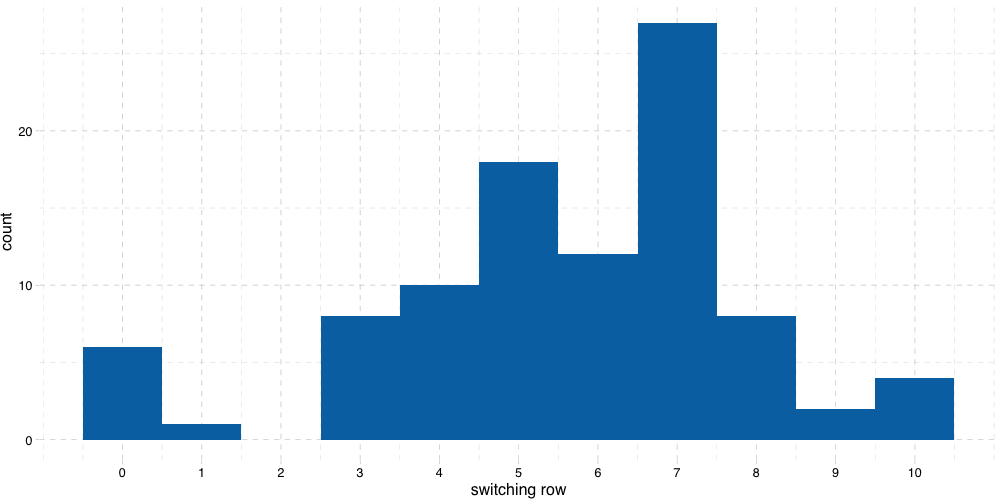
\includegraphics[scale=0.3]{graphs/hist_mpl.png}
    \caption{Histogram of Choice of Switching Row}
    \label{fig:hist_mpl}
\end{figure}


Participants did not seem to change their views on the fairness of the game. Figure \ref{fig:fairness_boxplot} shows a boxplot of their assessment at the beginning and at the end of the competition rounds with 0 being only luck and 7 being only skill that determined the outcome of the game. Table \ref{tab:fair_ols} lists the results of a linear regression. However, no characteristic shows any significant effect on the change in fairness sentiment.\\

\begin{figure}[H]
    \centering
    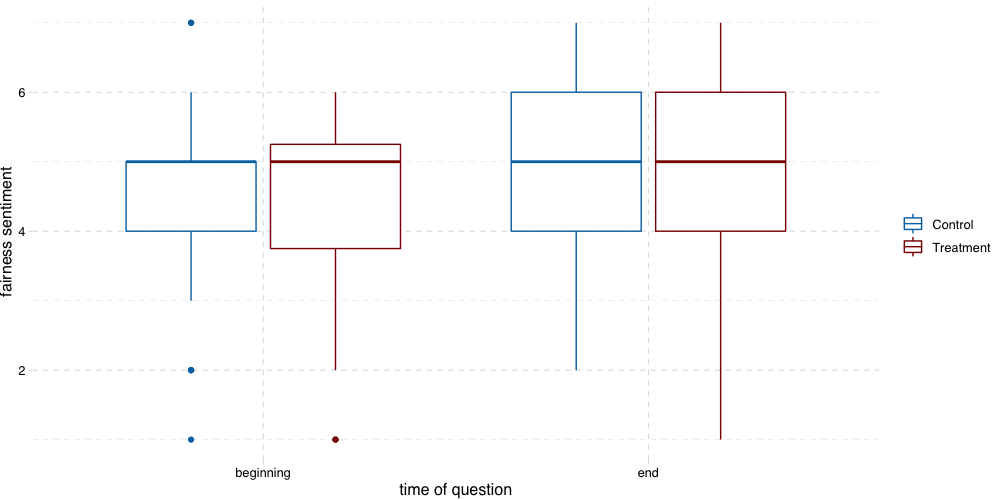
\includegraphics[width=\textwidth]{graphs/fairness_sentiment_boxplot.png}
    \caption{Fairness Sentiment Voting}
    \label{fig:fairness_boxplot}
\end{figure}



\begin{table}[!htbp] \centering 
  \caption{OLS Change in Fairness Sentiment} 
  \label{tab:fair_ols} 
   \scalebox{0.6}{%
\begin{tabular}{@{\extracolsep{5pt}}lc} 
\\[-1.8ex]\hline 
\hline \\[-1.8ex] 
\\[-1.8ex] & Change in Fairness Sentiment \\ 
\hline \\[-1.8ex] 
 treatment & $-$0.183 \\ 
  & (0.391) \\ 
  & \\ 
 payoff & 0.015 \\ 
  & (0.052) \\ 
  & \\ 
 CRT score & 0.063 \\ 
  & (0.188) \\ 
  & \\ 
 risk aversion & 0.013 \\ 
  & (0.084) \\ 
  & \\ 
 gender (male) & $-$0.181 \\ 
  & (0.366) \\ 
  & \\ 
 valuation & 0.048 \\ 
  & (0.063) \\ 
  & \\ 
 Constant & $-$0.971 \\ 
  & (1.298) \\ 
  & \\ 
  \hline
Observations & 96 \\ 
R$^{2}$ & 0.016 \\ 
Adjusted R$^{2}$ & $-$0.051 \\ 
Residual Std. Error & 1.733 (df = 89) \\ 
F Statistic & 0.235 (df = 6; 89) \\ 
\hline \\[-1.8ex] 
\hline 
\textit{Notes:} & \multicolumn{1}{l}{$^{*}$p$<$0.1; $^{**}$p$<$0.05; $^{***}$p$<$0.01} \\ 
% & \multicolumn{1}{l}{$^{**}$Significant at the 5 percent level.} \\ 
% & \multicolumn{1}{l}{$^{*}$Significant at the 10 percent level.} \\ 
\end{tabular} 
}
\end{table} 

\section{Hypotheses Testing}

In this section, we will look at the results regarding, first, the distribution of probabilities and its change across rounds, and, second, the factors affecting the probability of winning for a given individual according to the hypotheses postulated in section \ref{sec:hyp}.


\subsection{Hypotheses 1 and 2}

\textbf{Hypothesis \ref{hyp:treat}:} \textit{Mean investments will be higher than the expected profit maximizing value for all treatments, but will decrease over time.}\\ 
\textbf{Hypothesis \ref{hyp:treat-overinvest}:} \textit{Participants in the treatment group will invest a smaller multiple of their optimal investment.}\\

The first step needed to test these hypotheses is to determine the optimal investment value for each participant. Running a t-test on the hypothesis that the distance to the mean of valuations is 0, in other words, that there is no difference in valuation between participants, supports this assumption (p = 1 for control and p = 0.85 for the treatment). This result greatly simplifies the process by allowing the use of formula \ref{eq:opt_last}.\\

Furthermore, since the treatment and control groups have different valuations, to more easily compare the results I analyze the mean difference over optimal investment for both groups instead of the nominal amount of over-investment. Note that the valuation for the treated groups is calculated from the difference in the taxed benchmark rounds as explained in section \ref{ss:tax_bench}.\\

Consistent with expectations, participants bid on average significantly more than their optimum but decreasingly so over time, as Figure \ref{fig:over_invest} shows. It plots each round to the mean per treatment of the over investment ratio, i.e., how many times more than the optimum was invested on average.\\

Interestingly, participants in the taxation treatment invest both nominally and relatively more than those in the control, with treatment participants bidding on average 5 and a half times their optimal investment in the first round and 2.3 times their optimum in the last round. Participants in the control, on the other hand, invest from 1.93 times their optimum in the first round, to 1.36 times in the last round.\\


\begin{figure}
    \centering
    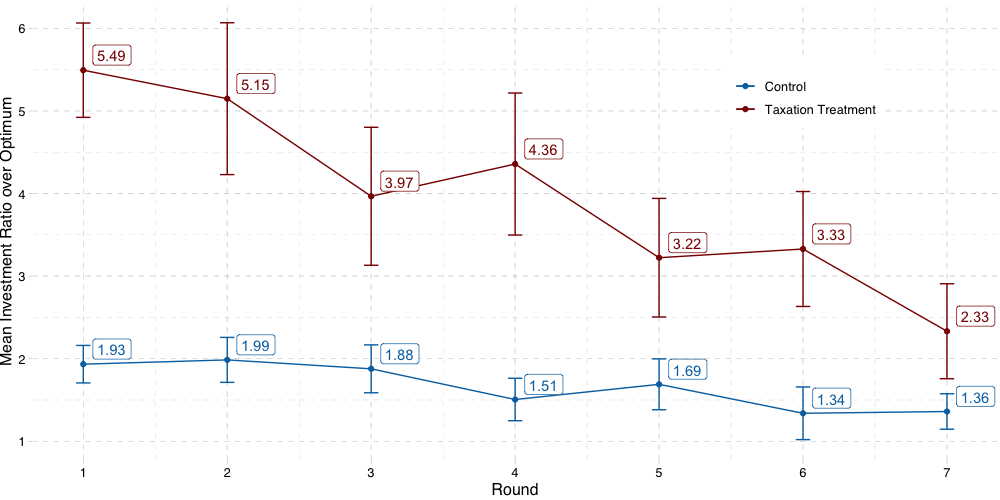
\includegraphics[width=\textwidth]{graphs/over_invest.png}
    \caption{Ratio of Over Investment per Round}
    \label{fig:over_invest}
\end{figure}


A possibility for why participants in the treatment invest relatively more is that subjects in both groups apply a simple heuristic of a given proportion of available income to invest. Given the fact that taxed players have a lower valuation but a higher disposable income, their bids are a higher proportion of the optimum. Running a regression on the investment ratio of available income in fact deletes the effect of all fixed effects but time, suggesting that participants tend to invest the same amount of their available income, regardless of their earnings or idiosyncratic features (see Table \ref{ax:available_share}). Figure \ref{fig:invest_share} shows a plot of the mean shares of the available income invested. The shares decrease with time in similar fashion for both treatments and, apart from the final investing round, within a standard error from each other.\\

\begin{figure}[H]
    \centering
    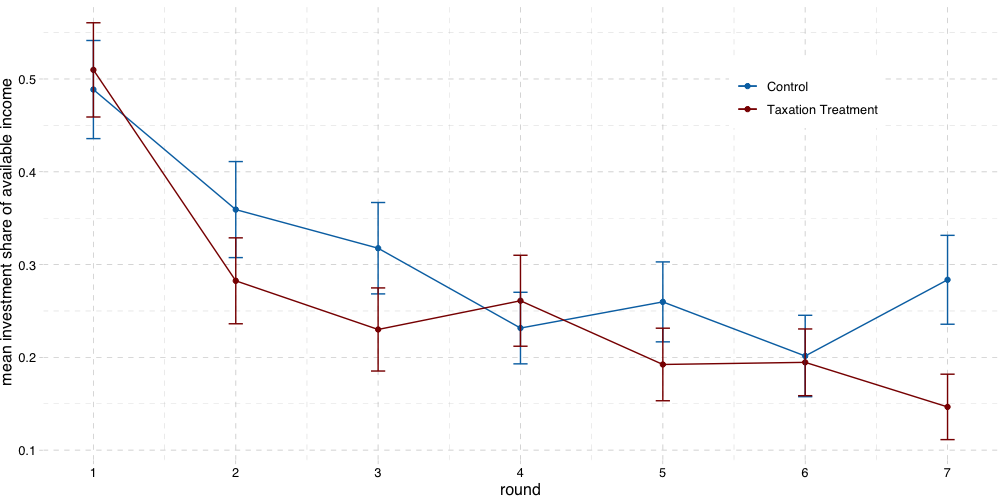
\includegraphics[width=\textwidth]{graphs/investment_share_geom_line.png}
    \caption{Investment Share of Available Income per Round}
    \label{fig:invest_share}
\end{figure}

Table \ref{tab:over_invest} presents a linear mixed model dissecting the most important causes for over-investing. The random effects are \textit{participants} nested in \textit{group}s.\\

The first and second models have a total explanatory power of around 52\% (conditional R-squared) in which the fixed effects of the first explain 10.03\% and the second 14.5\% of the variance (marginal R-squared). The effect of the treatment is significant and large for both models with participants investing, contrary to hypothesis \ref{hyp:treat-overinvest}, almost double as much over the optimum as subjects in the control group. Round repetition and risk averse behavior have both a significant, although relatively small, effect in the expected negative direction. The CRT score and whether a participant was playing with a high wage did not have a significant effect on the over-investment ratio.\\

\begin{table} 
\centering 
  \caption{Linear Mixed Model: Over Investment Ratio} 
  \label{tab:over_invest}
  \scalebox{0.6}{%
\begin{tabular}{@{\extracolsep{5pt}}lcc} 
\\[-1.8ex]\hline 
\hline \\[-1.8ex] 
\\[-1.8ex] & \multicolumn{2}{c}{Ratio of Investment Over Optimum} \\ 
\\[-1.8ex] & (1) & (2)\\ 
\hline \\[-1.8ex] 
 treatment & 2.314$^{***}$ & 2.075$^{***}$ \\ 
  & (0.698) & (0.678) \\ 
  & & \\ 
 round & $-$0.307$^{***}$ & $-$0.307$^{***}$ \\ 
  & (0.055) & (0.055) \\ 
  & & \\ 
 was winner & 0.256 & 0.281 \\ 
  & (0.271) & (0.271) \\ 
  & & \\ 
 CRT score &  & $-$0.183 \\ 
  &  & (0.289) \\ 
  & & \\ 
 risk aversion &  & $-$0.375$^{***}$ \\ 
  &  & (0.126) \\ 
  & & \\ 
 gender (Male) &  & 0.284 \\ 
  &  & (0.583) \\ 
  & & \\ 
 Constant & 2.813$^{***}$ & 5.689$^{***}$ \\ 
  & (0.546) & (1.097) \\ 
  & & \\ 
  \hline
  \hline
Observations & 672 & 672 \\ 
Log Likelihood & $-$1,751.726 & $-$1,747.753 \\ 
Akaike Inf. Crit. & 3,517.453 & 3,515.506 \\ 
Bayesian Inf. Crit. & 3,549.024 & 3,560.608 \\
\hline
Var: participant|group (Intercept) & 5.66 &     5.17     \\
Var: group (Intercept)           & 1.62  &    1.48    \\
Var: Residual                              & 8.14   &   8.14    \\
\hline \\[-1.8ex] 
\textit{Notes:} & \multicolumn{2}{r}{$^{*}$p$<$0.1; $^{**}$p$<$0.05; $^{***}$p$<$0.01} \\ 
% & \multicolumn{2}{l}{$^{**}$Significant at the %5 percent level.} \\ 
% & \multicolumn{2}{l}{$^{*}$Significant at the %10 percent level.} \\ 
\end{tabular}
}
\end{table}


Figure \ref{fig:beliefs_smooth} plots the differences between the estimation made by participants before the investment round and the actual investments  made. A perfect guess would be located at 0 in the y-axis. In the plot, a reduction in the mean over-estimation can be seen. It indicates better knowledge of other's behaviour with progressing rounds. It is nevertheless surprising how little accuracy participants appear to gain even after playing seven rounds and having been shown all relevant information.\\

\begin{figure}
    \centering
    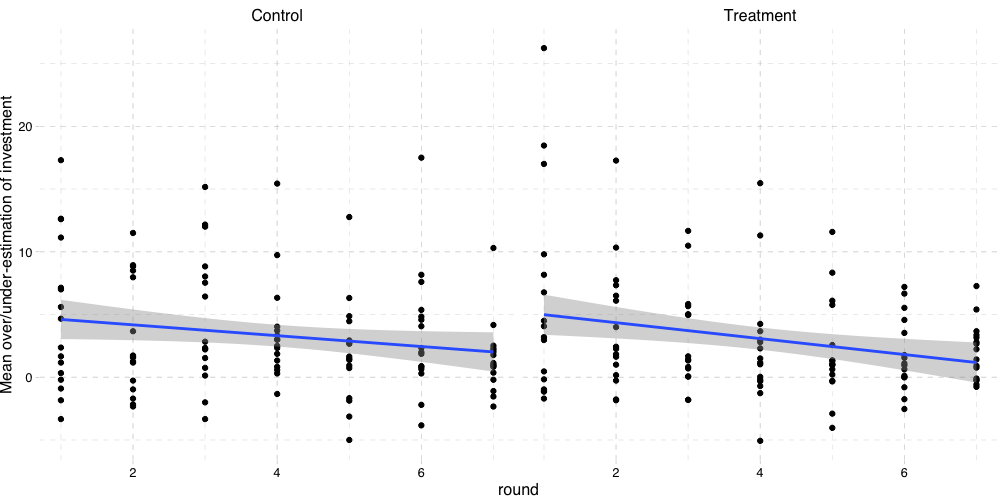
\includegraphics[width=\textwidth]{graphs/beliefs_smooth_lm.png}
    \caption{Mean Absolute Over or Under-estimation of Other's Investments by Group and Round}
    \label{fig:beliefs_smooth}
\end{figure}

A Wilcoxon rank test (p = 0.01) suggests, furthermore, that total welfare (the total amount of tokens paid out during competition) is larger in the treatment than in the control. Higher welfare in the treatment seems to be driven by working closer to the optimum.\\ 
%Adding the Gini coefficient of the available income to the model in table \ref{tab:over_invest} does not show any significance of inequality nor does it change the remaining coefficients which strengthens the idea that the higher investment in the treatment is due to an available income share heuristic.\\

\subsection{Hypothesis 3}

\textbf{Hypothesis \ref{hyp:wins}:} \textit{The coefficient of variation of winning probabilities will be increasing across rounds while being smaller in the treatment group.}\\

Participants appear to invest less with each round as the histogram in Figure \ref{fig:invest_hist} shows. Indeed, several participants do not invest anything at all and their number increases with each repetition which leads to the pattern shown in Figure \ref{fig:invest_prob_point}: With increasing rounds, the relationship between the invested amounts and the probability obtained grow apart. This means, in particular, that with each passing round, more lower investments had a higher probability of winning.\\

\begin{figure}[H]
    \centering
    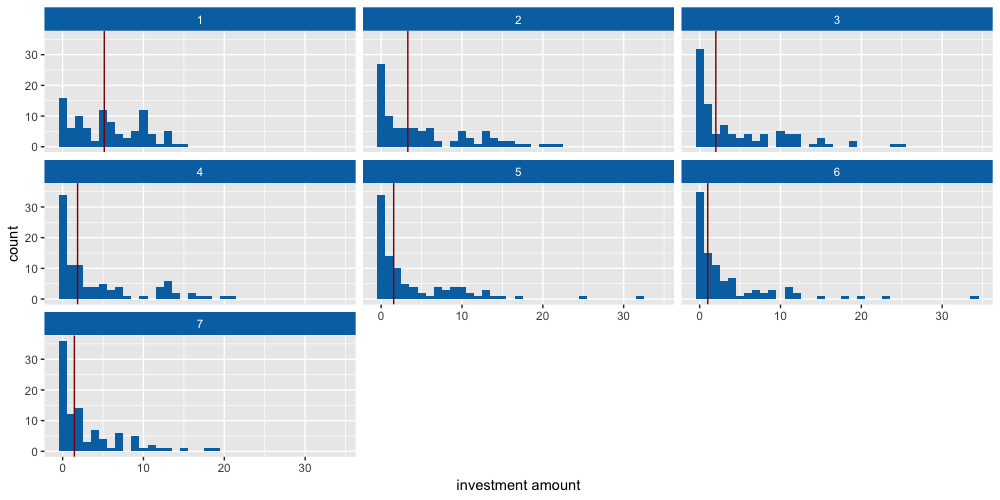
\includegraphics[scale=0.4]{graphs/investment_amount_hist.png}
    \caption{Histogram of Investment Amounts by Round. The Red Line Demarks the Median of the Distribution.}
    \label{fig:invest_hist}
\end{figure}

\begin{figure}[H]
    \centering
    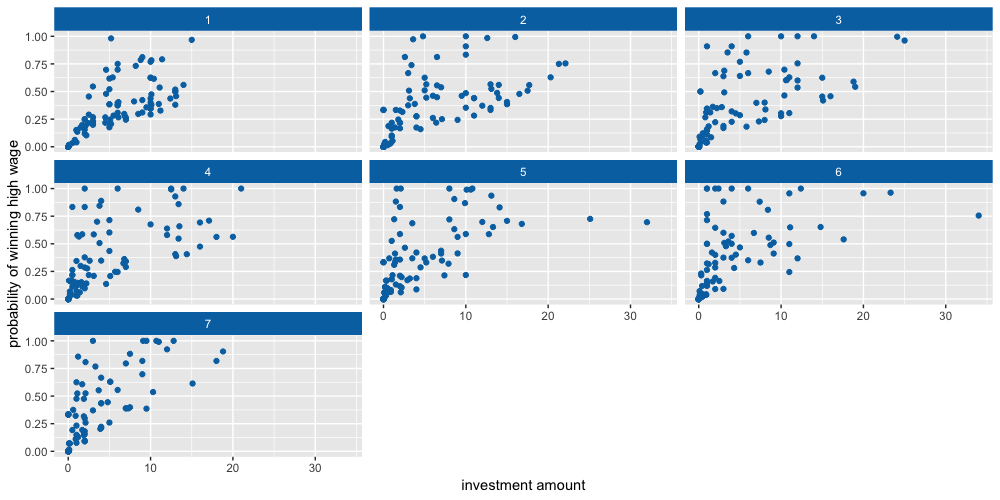
\includegraphics[scale=0.4]{graphs/invest_prob_point.png}
    \caption{Plot of the Probability Achieved by a Given Investment per Round}
    \label{fig:invest_prob_point}
\end{figure}

In terms of probabilities, I am interested in how their distribution change. Naturally, the mean probability of earning the high wage is always equal to $1/n$, but its distribution can vary from exactly $1/n$ for each participant, to only one person in the group having a probability of 1 and all the rest a probability of 0. Figure \ref{fig:dens_prob} shows the density plots for each round. A completely equal distribution would have its maximum at 0.33 with no values around it, while a completely unequal distribution would see two peaks at each extreme with the one at 0 being twice the size of the the one at 1.\\

\begin{figure}[H]
    \centering
    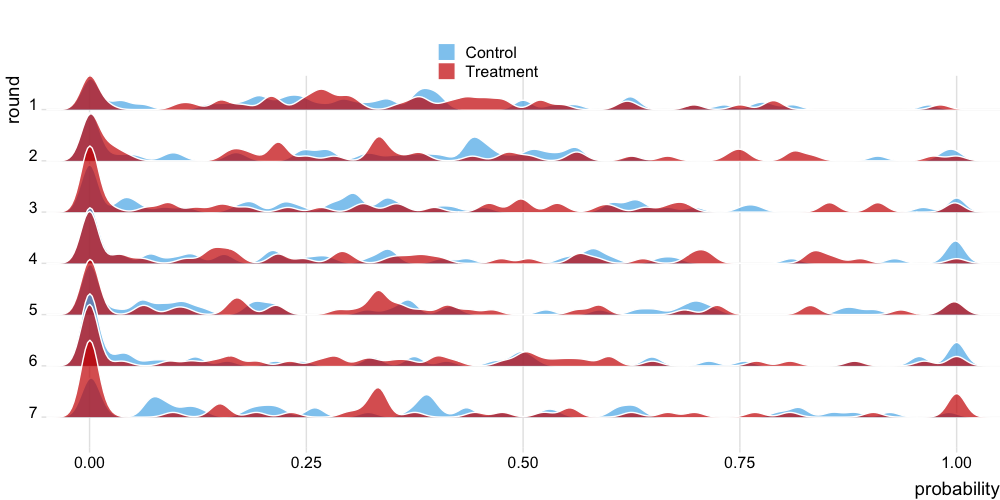
\includegraphics[width = \textwidth]{graphs/density_ridge_prob.png}
    \caption{Density Plots of Probability across Rounds}
    \label{fig:dens_prob}
\end{figure}

Figure \ref{fig:dens_prob} seems, in fact, to show an increase of density at the ends of the distribution with round 1 having a rather flat shape and round 7 stronger peaks at both 0 and 1 probability. Figure \ref{fig:var_coeff_boxplot} shows a box plot of the coefficient of variations across rounds for both treatments. In fact, it seems to increase across rounds but not significantly between treatments.\\

\begin{figure}[H]
    \centering
    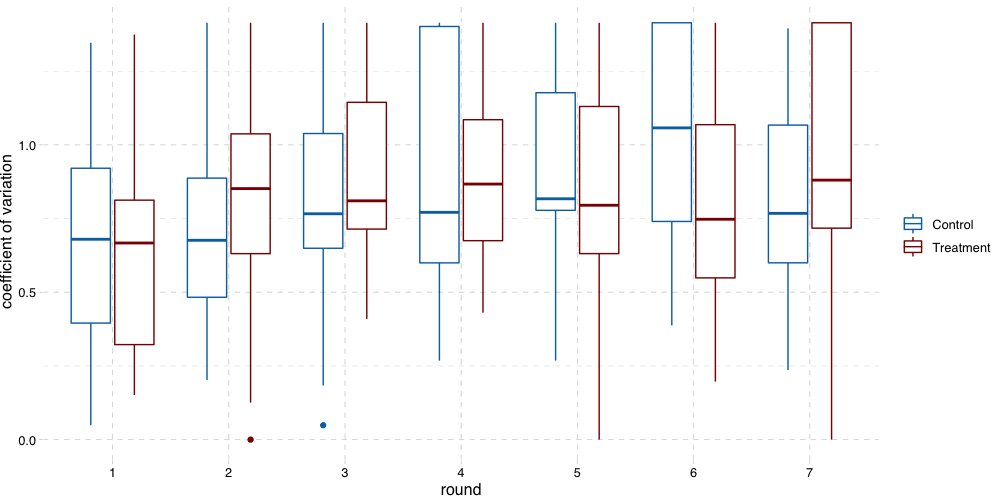
\includegraphics[width = 0.8\textwidth]{graphs/var_coeff_prob_boxplot.png}
    \caption{Boxplot Coefficient of Variation}
    \label{fig:var_coeff_boxplot}
\end{figure}

Table \ref{tab:var_coeff_ols} shows the results for an OLS regression of two models explaining the difference across groups in the coefficient of variation for the probabilities of winning. A linear mixed model is left out here since each group is part of only one treatment and the variables are all aggregated at the group level. Only round repetition appears to have a significant, although small effect (in our setting, the coefficient of variance can fluctuate between 0 and 1.73) on the coefficient of variation. Idiosyncratic group values like the mean value of valuation, CRT score or risk aversion do not play a significant role in the variation of probabilities. Taxation and redistribution also do not play a role. In other words, introducing a redistribution scheme does not avoid the fact that, with time, the distribution of probabilities will go to extremes with some participants having most of the chance to win and the rest having almost none.\\

\begin{table}[!htbp] \centering 
  \caption{OLS Coefficient of Variation} 
  \label{tab:var_coeff_ols} 
\begin{tabular}{@{\extracolsep{5pt}}lcc} 
\\[-1.8ex]\hline 
\hline \\[-1.8ex] 
\\[-1.8ex] & \multicolumn{2}{c}{Coefficient of Variation} \\ 
\\[-1.8ex] & (1) & (2)\\ 
\hline \\[-1.8ex] 
 treatment & $-$0.025 & $-$0.031 \\ 
  & (0.063) & (0.065) \\ 
  & & \\ 
 round & 0.043$^{***}$ & 0.043$^{***}$ \\ 
  & (0.016) & (0.016) \\ 
  & & \\ 
 mean CRT score &  & 0.092 \\ 
  &  & (0.059) \\ 
  & & \\ 
 mean risk aversion &  & $-$0.020 \\ 
  &  & (0.025) \\ 
  & & \\ 
 mean valuation &  & $-$0.033 \\ 
  &  & (0.023) \\ 
  & & \\ 
 Constant & 0.856$^{***}$ & 1.218$^{***}$ \\ 
  & (0.077) & (0.338) \\ 
  & & \\
  \hline
Observations & 224 & 224 \\ 
R$^{2}$ & 0.034 & 0.053 \\ 
Adjusted R$^{2}$ & 0.025 & 0.031 \\ 
Residual Std. Error & 0.468 (df = 221) & 0.467 (df = 218) \\ 
F Statistic & 3.857$^{**}$ (df = 2; 221) & 2.431$^{**}$ (df = 5; 218) \\ 
\hline
\hline \\[-1.8ex] 
\textit{Notes:} & \multicolumn{2}{r}{$^{*}$p$<$0.1; $^{**}$p$<$0.05; $^{***}$p$<$0.01} \\ 
% & \multicolumn{2}{l}{$^{**}$Significant at %the 5 percent level.} \\ 
% & \multicolumn{2}{l}{$^{*}$Significant at the %10 percent level.} \\ 
\end{tabular} 
\end{table}


Of course, this does not tell us much about what determines the probability of a given participant to win a contest. To analyze it, I suggest again a linear mixed model, although this time a generalized mixed model from a beta distribution as the results represent a distribution of probabilities with values restricted from 0 to 1\citep[Chapter~17]{krishnamoorthy2016}.\footnote{Since several participants did not invest at all and thus had a probability of winning of 0, this led to some other participants having a probability of winning of 1. Those values were transformed to 0.0000000000001 and 0.0000000000009 respectively to allow them to fit a beta distribution. The analysis was conducted with the \textit{glmmTMB} package \citep{brooks2017}.} Table \ref{tab:glm_prob} shows the results.\\

The only variable that shows a significant, although small, effect on the probability of winning is the size of the available income. Note, in particular, that having won alone has no significant effect on the probability of winning. This is in part because participants who are working with the lower rate can still achieve a large available income if they switch above their optimal point and thus forfeit time in the leisure mode. An alternative model including cumulative wins also showed no influence on the probability of winning.\footnote{The regression table is in the Appendix \ref{ax:glm_prob}.}\\

\begin{table}[!htbp] \centering 
  \caption{GLMM Probability of Winning} 
  \label{tab:glm_prob} 
  \scalebox{0.6}{%
\begin{tabular}{@{\extracolsep{5pt}}lcc} 
\\[-1.8ex]\hline 
\hline \\[-1.8ex] 
\\[-1.8ex] & \multicolumn{2}{c}{Probability of Winning} \\ 
\\[-1.8ex] & (1) & (2)\\ 
\hline \\[-1.8ex] 
 treatment & $-$0.139 &  $-$0.087241 \\ 
  & (0.22) & (0.218) \\ 
  & & \\ 
 available income & 0.045$^{***}$ & 0.045$^{***}$ \\ 
  & (0.008) & (0.008) \\ 
  & & \\ 
 was winner & $-$0.084 &  $-$0.083 \\ 
  & (0.119) & (0.119) \\ 
  & & \\ 
 gender (male) &  & 0.356 \\ 
  &  & (0.223) \\ 
  & & \\ 
 CRT score &  & $-$0.051 \\ 
  &  & (0.113) \\ 
  & & \\ 
 risk aversion & & $-$0.034 \\ 
  &  & (0.049) \\ 
  & & \\ 
 valuation &  & 0.056 \\ 
  &  & (0.038) \\ 
  & & \\ 
 mean investment belief &  & 0.003 \\ 
  &  & (0.008) \\ 
  & & \\ 
 Constant & $-$1.413$^{***}$ & $-$2.454$^{***}$ \\ 
  & (0.209) & (0.647) \\ 
  & & \\ 
  \hline
Observations & 672 & 672 \\ 
Log Likelihood & 3798.4 & 3801.0 \\ 
Akaike Inf. Crit. & $-$7580.9 & $-$7575.9 \\ 
Bayesian Inf. Crit. & $-$7544.8 & $-$7517.3 \\
\hline
Num. groups: participant:group     & 96     &   96   \\
Num. groups: group               & 32      &    32  \\
Num. groups: round                         & 7   & 7        \\
\hline
Var: participant:group (Intercept) & 0.93   & 0.02     \\
Var: group (Intercept)           & 0.00   & 0.00     \\
Var: round (Intercept)           & 0.00    & 0.00    \\
Var: Residual                    & 0.00     &  0.02  \\
\hline
\hline \\[-1.8ex] 
\textit{Notes:} & \multicolumn{2}{l}{$^{*}$p$<$0.1; $^{**}$p$<$0.05; $^{***}$p$<$0.01} \\ 
% & \multicolumn{2}{l}{$^{**}$Significant at %the 5 percent level.} \\ 
% & \multicolumn{2}{l}{$^{*}$Significant at the %10 percent level.} \\ 
\end{tabular} 
}
\end{table} 
\thispagestyle{fancy}
\chapter{Discussion and Further Research}
\label{ch:discussion}

Since, to my knowledge, this is the first study of its type, the presented thesis starts from sensible parameters that can be adapted by future researchers to dive deeper into different aspects of the model. In this chapter, I list some of the questions that arose from the results, as well as suggest some design and parameter changes to answer them.\\

Changing, for instance, the difference between the high and low wages could lead to stronger reactions in work supply when winning, and to the sentiment of fairness of the game. Remember from section \ref{sec:budget_constraint} that given a high enough high valuation, losing players will have no possibility to invest their optimal investment. This could furthermore exacerbate the tendency of probabilities to grow apart from each other.\\

In a related manner, but presenting a more complex change to model, the prize can be increased with each passing round. Alternatively, the contest success function can be altered to be more or less deterministic by changing the exponent $r$ in the equation:

\begin{equation}
    p(I_i,I_{-i}) =
\begin{cases}
    \frac{1}{n},& \text{if } I_i = I_{-i} = 0\\
    \frac{I_i^r}{I_i^r + \sum_{j\neq i}^n I_{j}^r},              & \text{otherwise}
\end{cases}
\label{eq:csf_exp}    
\end{equation}

A result that also pointed the way to a design expansion was the apparent available income share heuristic. In future experiments, one could control, for instance, if participants are aware of how much the prize is worth by eliciting beliefs about the valuation of the game before the investment screen. This would further reveal how much of the over-investment is due to competition properties like last place aversion and winning utility. Likewise, the slider interface for investing could be changed to a number input which could help mitigate the visual effect of choosing a share of the available income instead of a particular value that maximizes expected earnings.\\

A comparison between the present design, which included full information about the participant's own performance as well as the performance of others, and a treatment with no information could also help to disentangle the impact of learning, a decreasing utility function for winning, as well as competition properties like inequality or last place aversion.\\

In the same manner, a specific workaround to the problem posed in chapter \ref{ss:compt} could have been to add two rounds without an investment or prize option, but with information about the performance of group members. However, this could nevertheless have been used by a participant to send signals about their own valuation of the prize to other participants. Since a participant with a higher valuation would also invest more, sending signals about his or her own valuation might be rewarding even if no prize is to be immediately won. But considering, as shown in section \ref{sec:budget_constraint}, that participants will always be able to invest their optimal amount, the impact of this in the present thesis would have been moderate. Given a high prize, however, the effect would be significant.\\

Other parameter changes that might have a strong repercussion -- the modelling of which is beyond the scope of this thesis -- are, for instance, the number of people in the group or the number of winners per round. Furthermore, one could model the invested amounts as a public good, in a similar way as investment in education works in the real world, such that the investments are either redistributed to the winner(s) or to the entire community.\\

On the policy end, looking back at the original postulates of the Prospect of Upward mobility, it is difficult to make a prediction as to which way voting would go in a dynamic setting. Considering that the majority of probabilities tended to go to 0, we could expect voting for taxing to go up in the long run. On the other hand, as smaller investments also lead to higher probabilities of winning with increasing rounds, taxation could be voted down whenever players have a positive probability of obtaining the prize. Which of the two directions dominates will be strongly dependant on the determinism of the contest expressed through the exponent $r$ of equation \ref{eq:csf_exp} and the valuation of the prize. A design that internalizes both voting on taxation and the POUM would be an interesting way to see how these two factors play into each other, but it would require a better knowledge of the dynamics of several taxation schemes and $r$ parameters beforehand.\\

Finally, an issue of extreme importance that could not be addressed in this thesis is the efficiency of the wins. One could argue that ideally, the participant who wins the contest should be the one who gets the most out of it i.e. the one who earns the most under the high piece rate. This kind of efficiency could also be interpreted as fairness since it not only maximises total welfare but awards the prize to the most deserving participant. It could be perceived as fair, particularly when investments and income are reinvested in the form of a public good. The current design and analysis assumes an equal valuation among participants due in large part to the selection of the real effort task and the relatively low valuation of the prize. Adjusting the difference in wages between winners and losers and calculating the optimal investments according to equation \ref{eq:InvDiffVal} would make it possible to judge the efficiency of the wins and help find interventions that foster fairness.\\

Many other changes and extensions are possible which will hopefully help to better understand the dynamics of Tullock contests in various real-world scenarios, from public education, to the labor market and the provision of public goods.\\

\chapter{Conclusion}
\label{ch:conclusion}

This thesis presented an experimental design aimed at analysing the dynamics of inequality, taxation, and redistribution, in a repeated Tullock Contest with full information given to the participants. It differs from other repeated rent-seeking contests in that the groups are kept equal and the prize is expressed in a higher wage for the next working period. In other words, the prize of the contests allows the winner to earn more and increase his or her available income, or to spend more leisure time while keeping earnings constant. This system made income inequality endogenous to the group. Moreover, in the treatment group, a redistribution scheme was introduced in order to test the effects of taxation on effort.\\

The results of the experimental sessions both confirmed and contradicted some of the initial hypotheses regarding the distribution of probabilities and the dynamics of investments. Consistent with previous literature, participants across treatments invested more than their respective optimal amounts. In particular, in the experiment I found that participants tend to invest a fixed amount of their available income, regardless of the potential win. Since participants in the taxation treatment have a larger available income but lower expected income, taxed participants invest a relatively larger amount.\\

Although it is not possible to pin-point the mechanism behind this heuristic (anchorage, endowment effect, etc.), the result suggests that redistributing assets to be invested in Tullock-like contests would increase, rather than decrease, inefficiency by over-investing.\\  

Over time, investment does decrease. This leads, on the one hand, to smaller investments carrying a greater probability of winning and, on the other, to a more skewed distribution of winning probabilities with more and more participants with either a very low or very high chance of obtaining the prize. This effect was observed in both treatments suggesting that the redistribution of income does not necessary lead to fairer distribution of opportunity in Tullock-like contests.\\

The overall results of the thesis suggest, in summary, that not only do Tullock-like contests induce great inefficiencies, but that the game organiser, the State for instance, could even exacerbate the problem by increasing available income. Taxation, however, reduces over-exertion of effort and reduces inefficiencies through that channel. The impact of the voting on taxation would likely depend on the deterministic index of the contest function. A contest function that awards higher weight to the invested amount would make it more difficult for those with less available income to win. They would, according to the Prospect of Upward Mobility, be more inclined to implement a taxation and redistribution scheme.\\

From this perspective, programs like student loan schemes can be viewed critically as they induce people to invest more than their expected return. Analogously, programs that tax investment could help reduce inefficiencies. It would be advisable, however, to redistribute through investments in non-investable assets, like infrastructure, to avoid the problem of increased available income.\\

The study of repeated Tullock contests is essential in understanding the dynamics of many group selection processes. Education and work promotions are two of the most prominent examples. With this thesis, I hope to have provided a glimpse into the ramifications of possible design changes and how these can be used to create more fair and more efficient competition.
%input{AKS} %Hauptquelle: originalarbeit, noch was?!
%\input{Versus}
\thispagestyle{fancy}

\begin{appendices}

\chapter{Derivations}
\label{ax:derivations}

\section*{Investment Optimization in Tullock Contests}

A player $i$ wants to find the $I^*$ that maximizes his or her expected profit as expressed in the maximization problem:


\begin{equation}
    \underset{I_i}{\text{max}}\quad\mathbb{E}\Pi_i(I_i,I_j) = \frac{I_i}{I_i + \sum_{j\neq i}^n I_{j}}\mathbb{V} - I_i
\label{eq:exp_util_anex}
\end{equation}

Here, $n$ is the  number of participants in the game.\\
Let us assume that the valuation of the game $\mathbb{V}$ is equal for all players and hence, that the optimal investment $I^{*}$ is equal for everyone. At the maximum of function \ref{eq:exp_util_anex} holds:
\begin{flalign*}
    \frac{d}{dI_i}(\frac{I_i\mathbb{V}}{I_i + \sum_{j\neq i}^n I_{j}} - I_i) = 0 &&
\end{flalign*}
which after deriving using the quotient rule results in:
\begin{flalign*}
    \frac{\mathbb{V}(I_i + \sum_{j\neq i}^n I_{j})-I_i\mathbb{V}}{(I_i + \sum_{j\neq i}^n I_{j})^2}-1&&
\end{flalign*}
Since we know that at the maximum $I_i^{*}=I_{-i}^{*}=I^{*}$ holds, we can simplify:
\begin{flalign*}
    \frac{n\mathbb{V}I^*-\mathbb{V}I^*}{(nI^*)^2}-1 = 0&&
\end{flalign*}
We further simplify to:
\begin{flalign*}
    \frac{\mathbb{V}\bcancel{I^*}(n-1)}{n^2I^{\bcancel{*2}}} = 1&&
\end{flalign*}
Which gives equation \ref{eq:opt_last}:
\begin{flalign*}
    I^{*} = \frac{n-1}{n^2}\mathbb{V}
\end{flalign*}

\section*{Asymmetric Valuations}

An important conundrum that the approach presented in this thesis makes easier to solve than Koch's proposal \cite{koch2017} is a possible difference in valuation of the prize in terms of higher wage since participants with higher ability or higher utility from consumption will profit more from it. \cite{nti1999} shows that in the two player case:\\

\begin{quote}
    "The player who values the prize more expends more effort in equilibrium but both players allocate the same fraction of their valuations to the contest".\footnote{\citet[p.~419]{nti1999}.}
\end{quote}

To show this, we just need to write the FOC for the two players explicitly:\footnote{See Appendix \ref{ax:derivations} for a derivation of the FOC.}

\begin{equation*}
\begin{split}
    \frac{I_j}{(I_j + I_i)^2}\mathbb{V}_i-1 = 0 \\
    \frac{I_i}{(I_j + I_i)^2}\mathbb{V}_j-1 = 0
\end{split}
\end{equation*}

By equalizing we obtain:
\begin{equation}
    \frac{I_i}{\mathbb{V}_i} = \frac{I_j}{\mathbb{V}_j} 
\end{equation}

Now let us consider the case of $n=3$ for $i \in (a,b,c)$ with exactly one winner.\footnote{\cite{stein2002} offers a general derivation for N players.} Using the same process as above we obtain the equation system:

\begin{align}
    \frac{(I_a+I_b)}{(I_a+I_b+I_c)^2}\mathbb{V}_c&=1\\
    \frac{(I_a+I_c)}{(I_a+I_b+I_c)^2}\mathbb{V}_b&=1\\
    \frac{(I_b+I_c)}{(I_a+I_b+I_c)^2}\mathbb{V}_a&=1
\end{align}

To more easily visualize the results, we assume w.l.o.g that $I_a = I$, $I_b = \beta_b I$ and $ I_c = \beta_c I $, and that $\mathbb{V}_a = \mathbb{V}$, $\mathbb{V}_b = \alpha_b \mathbb{V} $ and $\mathbb{V}_c = \alpha_c \mathbb{V}$. The equation system thus is simplified to:

\begin{align}
    \label{eq:sys1}\frac{(1+\beta_b)}{(1+\beta_b+ \beta_c )^2}\alpha_c\mathbb{V}&=I\\
    \label{eq:sys2}\frac{(1+\beta_c )}{(1+\beta_b  + \beta_c )^2}\alpha_b\mathbb{V}&=I\\
    \label{eq:sys3}\frac{(\beta_b +\beta_c )}{(1+\beta_b  + \beta_c )^2}\mathbb{V}&=I
\end{align}

After setting (\ref{eq:sys2}) = (\ref{eq:sys3}) we obtain:

\begin{equation}
    \label{eq:betab}\beta_b=(1+\beta_c)\alpha_b-\beta_c
\end{equation}

Similarly, we set (\ref{eq:sys1}) = (\ref{eq:sys3}) and obtain $(1+\beta_b)\alpha_c=\beta_b+\beta_c$ in which we can replace $\beta_b$ by (\ref{eq:betab}). Solving for $\beta_c$ we get:
\begin{equation}
\label{eq:betac}
    \beta_c = \frac{\alpha_b-\alpha_c-\alpha_b\alpha_c}{\alpha_b\alpha_c-\alpha_c-\alpha_b}
\end{equation}
Which inserted back in (\ref{eq:betab}) gives us:
\begin{equation}
\label{eq:betab2}
    \beta_b=\alpha_b + \alpha_b\frac{\alpha_b-\alpha_c-\alpha_b\alpha_c}{\alpha_b\alpha_c-\alpha_c-\alpha_b}-\frac{\alpha_b-\alpha_c-\alpha_b\alpha_c}{\alpha_b\alpha_c-\alpha_c-\alpha_b}
\end{equation}

Finally, from (\ref{eq:betab2}) and (\ref{eq:betac}) we know that $\beta_b+\beta_c = 1+\alpha_b\frac{\alpha_b-\alpha_c-\alpha_b\alpha_c}{\alpha_b\alpha_c-\alpha_c-\alpha_b}$ and we can replace in \ref{eq:sys3} to obtain:

\begin{equation}
\label{eq:InvDiffVal}
    I = \frac{\alpha_b+\alpha_b\frac{\alpha_b-\alpha_c-\alpha_b\alpha_c}{\alpha_b\alpha_c-\alpha_c-\alpha_b}}{(1+\alpha_b
    +\alpha_b\frac{\alpha_b-\alpha_c-\alpha_b\alpha_c}{\alpha_b\alpha_c-\alpha_c-\alpha_b})^2}\mathbb{V}
\end{equation}

\hfill \break

Now, to more easily see how this function behaves let us assume that only participant \textit{c} has a different valuation and therefore $\alpha_b = 1$. It follows:

\begin{equation}
    I_a=I_c=\frac{2\alpha_c}{(1+2\alpha_c)^2}\mathbb{V}
\end{equation}

The denominator will grow faster for increasing $\alpha_c$ which means that $I_a$ will tend to $0$.\\


The general case is more cumbersome but we can still find some conditions for the relationship between $\alpha_b$ and $\alpha_c$. Requiring that $\alpha_b, \alpha_c \in \mathbb{R}^+$ and that $\alpha_b\alpha_c-\alpha_c-\alpha_b \neq 0$, it can be shown that, in order for $I\geq0$, then $\alpha_b\alpha_c>\alpha_c+\alpha_b$.\\

This means, in particular, that there are some levels for which an investment is no longer profitable, take for instance $\alpha_b = 2$ and $\alpha_c = 4$.\\

A look at the function graph \ref{fig:invest_func} gives us a better understanding of its behavior. For very low levels of others' valuations the investment value is close to zero but increases with $\alpha_b$ and $\alpha_c$. After achieving a maximum of $\frac{1}{4}$, or the equivalent to the two player game, the function decreases monotonically.

\begin{figure}[H]
    \centering
    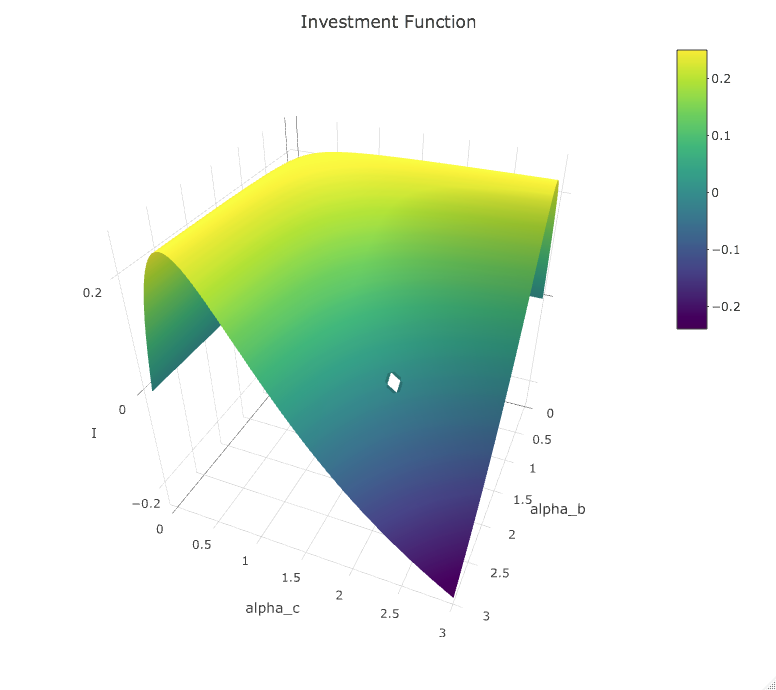
\includegraphics[scale=0.5]{graphs/Investment_Func.png}
    \caption{Investment function dependant on the share of others' valuation}
    \label{fig:invest_func}
\end{figure}

\chapter{Tables}

\begin{table}[!htbp] \centering
\begin{tabular}{@{\extracolsep{5pt}}lcc} 
\multicolumn{3}{l}{Wilcoxon rank sum test with continuity correction}\\
\\[-1.8ex]\hline 
\hline \\[-1.8ex] 
\multicolumn{1}{l}{Piece Rate} & \multicolumn{1}{c}{Statistic} & \multicolumn{1}{c}{p-value}\\
\hline \\[-1.8ex]
High & 1186.5 & 0.8006\\
Low & 1070 & 0.5462\\
\hline \\[-1.8ex] 
\hline \\[-1.8ex]
\multicolumn{3}{l}{\footnotesize{Null Hypothesis: Difference in production between treatments is equal to 0}}\\[2ex]
\end{tabular}
  \caption{Comparison of productions in the benchmarking rounds between treated and non-treated groups} 
  \label{tab:bench_prods_test} 
\end{table} 


    \begin{figure}
        \centering
        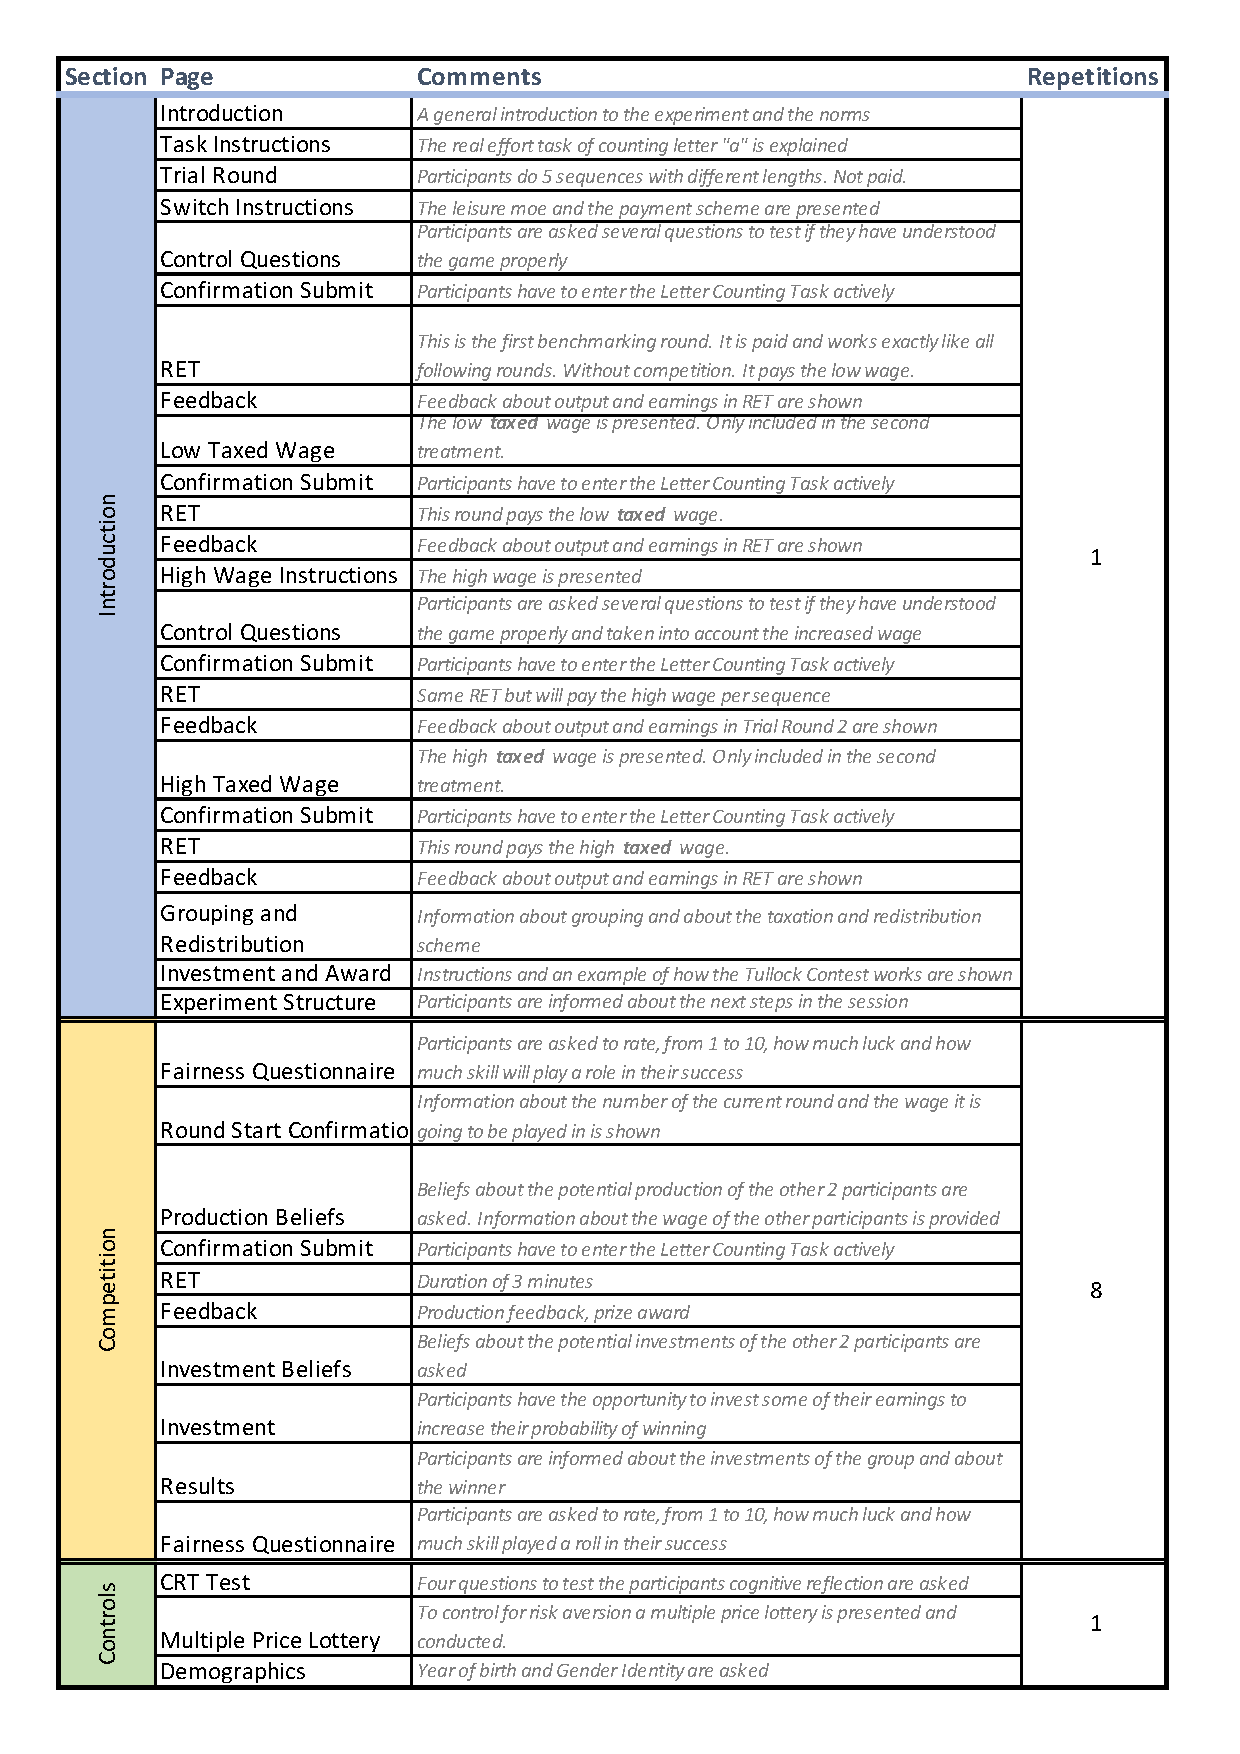
\includegraphics[width=\textwidth]{graphs/Experimental_Design.pdf}
        \caption{Detailed structure of the experiment}
        \label{tab:exp_design}
    \end{figure}
    
\begin{table}[!htbp] \centering 
  \caption{GLMM Probability of Winning} 
  \label{ax:glm_prob} 
\begin{tabular}{@{\extracolsep{5pt}}lc} 
\\[-1.8ex]\hline 
\hline \\[-1.8ex] 
\\[-1.8ex] & \multicolumn{1}{c}{Probability of Winning} \\ 
\\[-1.8ex] & (3)\\ 
\hline \\[-1.8ex] 
 treatment & $-$0.091 \\ 
  & (0.218) \\ 
  &  \\ 
 available income & 0.044$^{***}$  \\ 
  & (0.008) \\ 
  & \\ 
 was winner & $-$0.056 \\ 
  & (0.121) \\ 
  & \\ 
 gender (male) & 0.317\\ 
   & (0.225) \\ 
   & \\ 
 CRT score  & $-$0.036 \\ 
  & (0.113) \\ 
  & \\ 
 risk aversion & 0.036 \\ 
  & (0.049) \\ 
  & \\ 
 valuation & 0.060 \\ 
  & (0.038) \\ 
  & \\ 
 mean investment belief & 0.002 \\ 
  & (0.009) \\ 
  & \\
 cumulative wins & $-$0.037 \\ 
  & (0.028) \\ 
  & \\ 
 Constant & $-$2.364$^{***}$ \\ 
  & (0.650) \\ 
  & \\ 
  \hline
Observations & 672 \\ 
Log Likelihood & 3801.8 \\ 
Akaike Inf. Crit. & $-$7575.6 \\ 
Bayesian Inf. Crit. & $-$7512.5 \\
\hline
Num. groups: participant:group     &   96   \\
Num. groups: group               &    32  \\
Num. groups: round               & 7        \\
\hline
Var: participant:group (Intercept) &  0.872     \\
Var: group (Intercept) &          0.00     \\
Var: round (Intercept)  &          0.00    \\
\hline
\hline \\[-1.8ex] 
\textit{Notes:} & \multicolumn{1}{l}{$^{***}$Significant at the 1 percent level.} \\ 
 & \multicolumn{1}{l}{$^{**}$Significant at the 5 percent level.} \\ 
 & \multicolumn{1}{l}{$^{*}$Significant at the 10 percent level.} \\ 
\end{tabular} 
\end{table} 

\chapter{Screenshots}
\label{ax:screenshots}

\begin{figure}
\centering
\resizebox{1\columnwidth}{!}{%
\begin{tabular}{cc}
\subcaptionbox{Welcome Screen\label{1}}{
\includegraphics[width = 1.5in]{Screenshots/001-174-Welcome.png}} &
\subcaptionbox{Introduction Screen \label{2}}{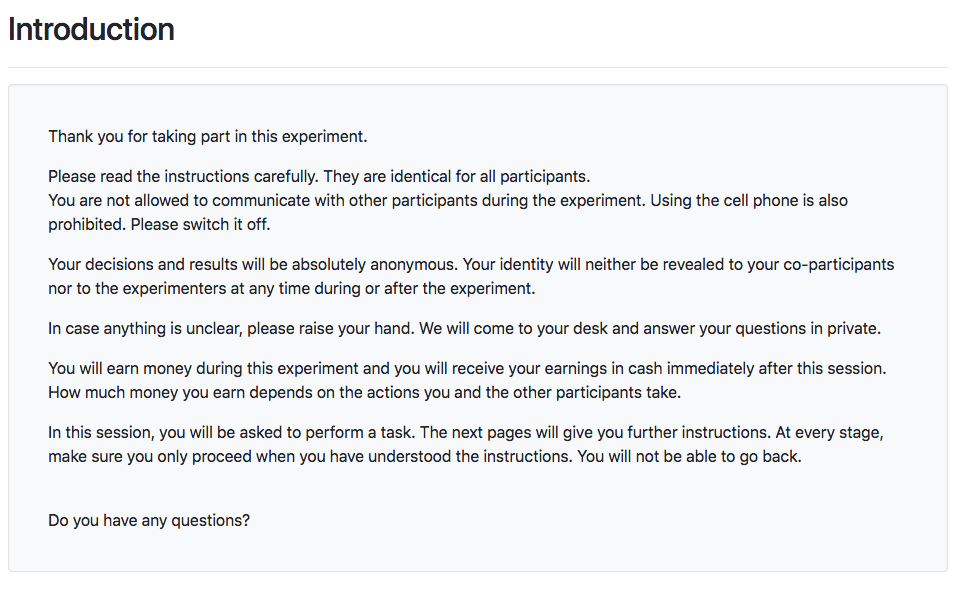
\includegraphics[width = 1.5in]{Screenshots/002-174-Introduction.png}} \\
\subcaptionbox{RET Instructions\label{3}}{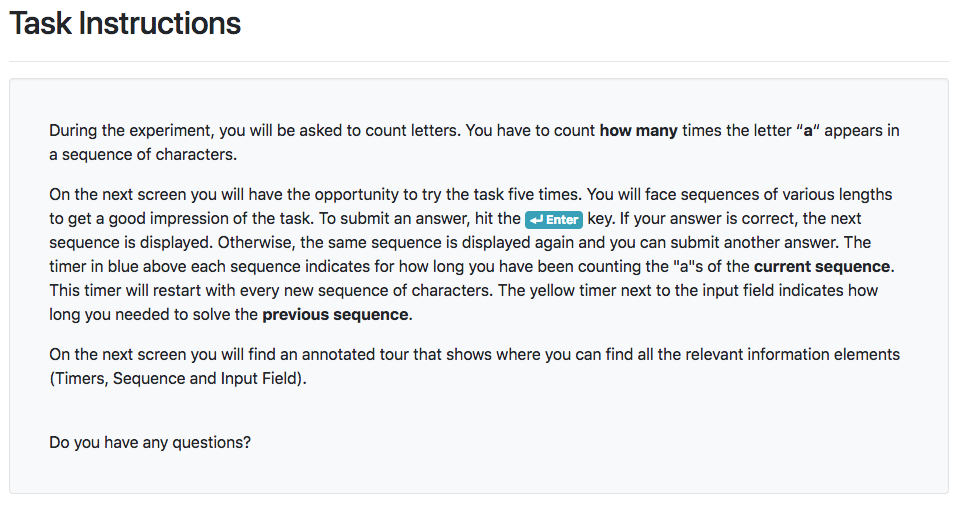
\includegraphics[width = 1.5in]{Screenshots/003-174-Instructions-Trial.png}}&
\subcaptionbox{Test Run Screen\label{4}}{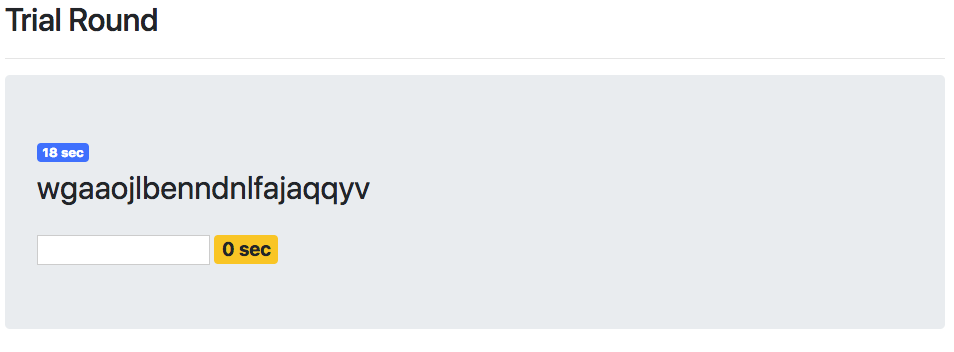
\includegraphics[width = 1.5in]{Screenshots/004-174-Trial-Task.png}} \\
\subcaptionbox{Payment Instructions Screen\label{5}}{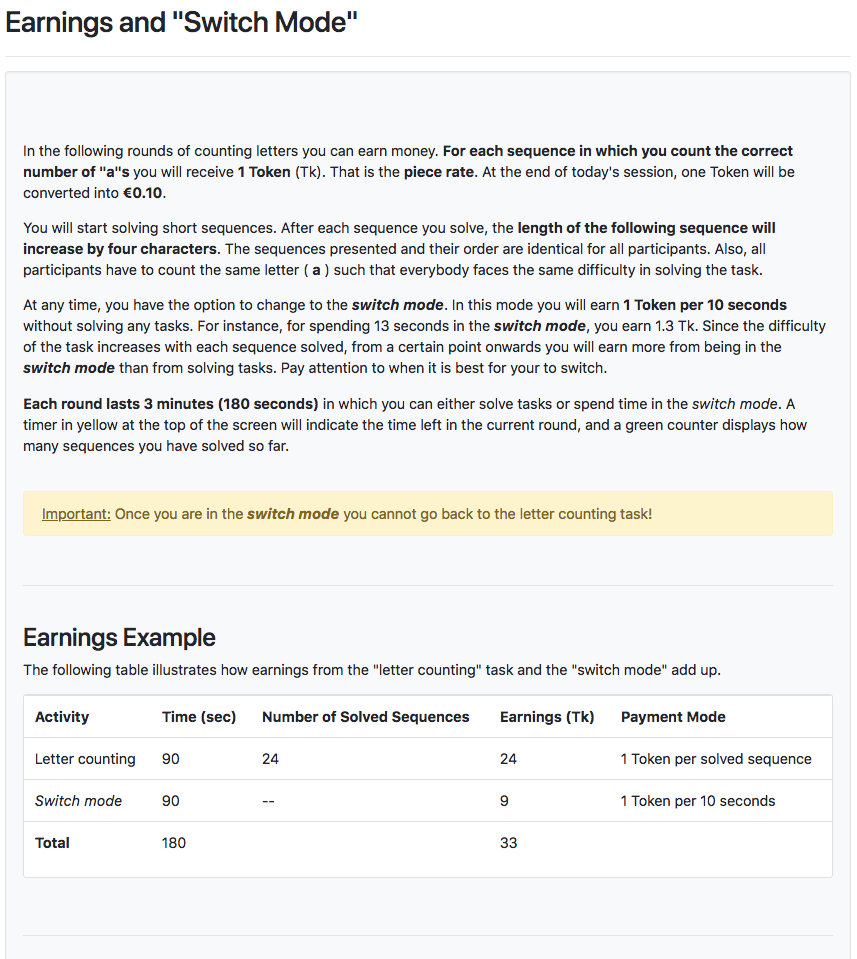
\includegraphics[width = 1.5in]{Screenshots/006-174-Switch_Instructions-1-2.png}} &
\subcaptionbox{Payment Instructions Screen\label{6}}{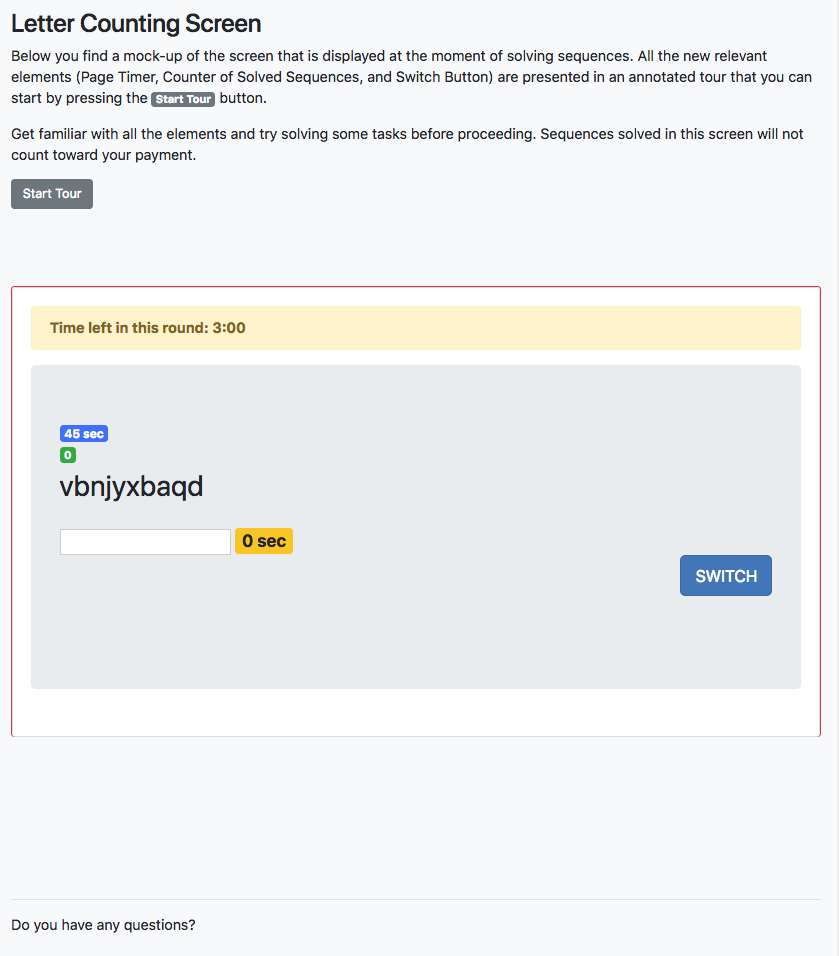
\includegraphics[width = 1.5in]{Screenshots/006-174-Switch_Instructions-2-2.png}}\\
\end{tabular}
}
\caption{Screenshot Selection}
\label{ax:screenshot_1}
\end{figure}

\begin{figure}
\centering
\resizebox{1\columnwidth}{!}{%
\begin{tabular}{ll}
\subcaptionbox{Control Questions\label{7}}{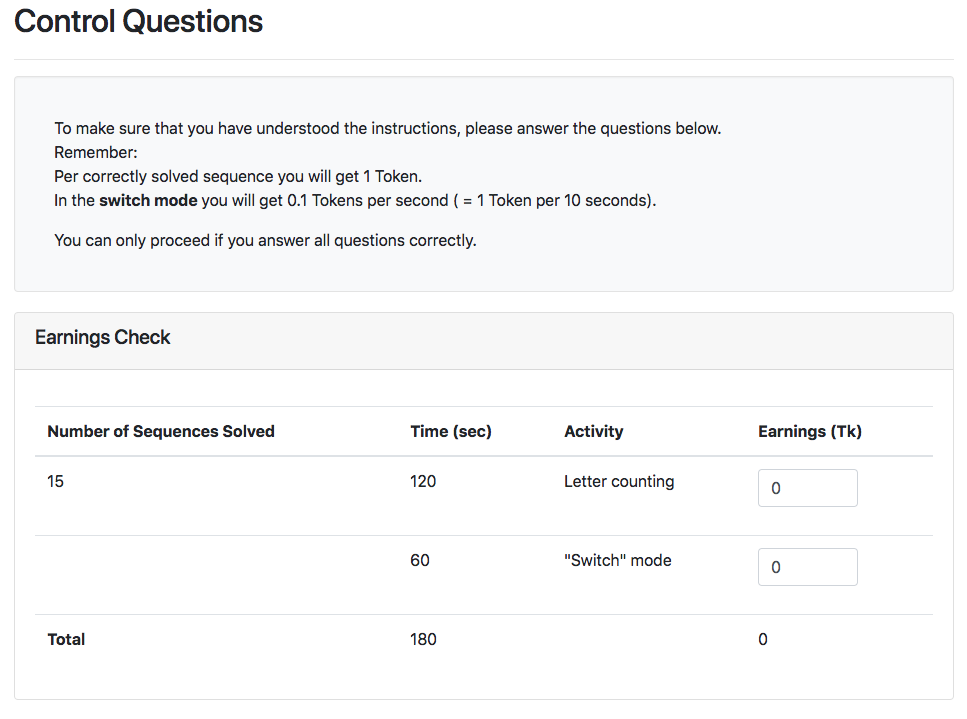
\includegraphics[width = 1.5in]{Screenshots/007-174-Control_Q_Low-1-2.png}} &
\subcaptionbox{Control Questions\label{8}}{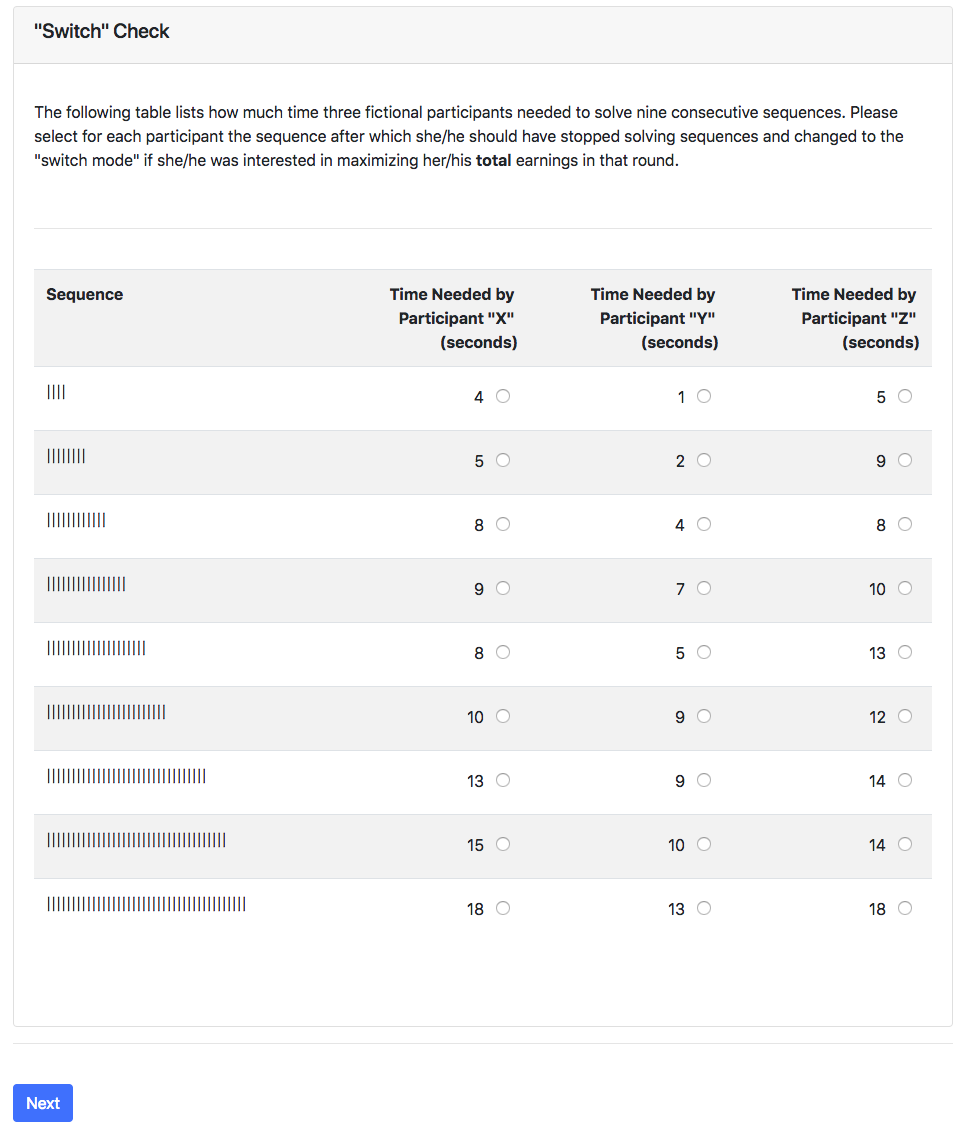
\includegraphics[width = 1.5in]{Screenshots/007-174-Control_Q_Low-2-2.png}} \\
\subcaptionbox{Start of Task Confirmation Screen\label{9}}{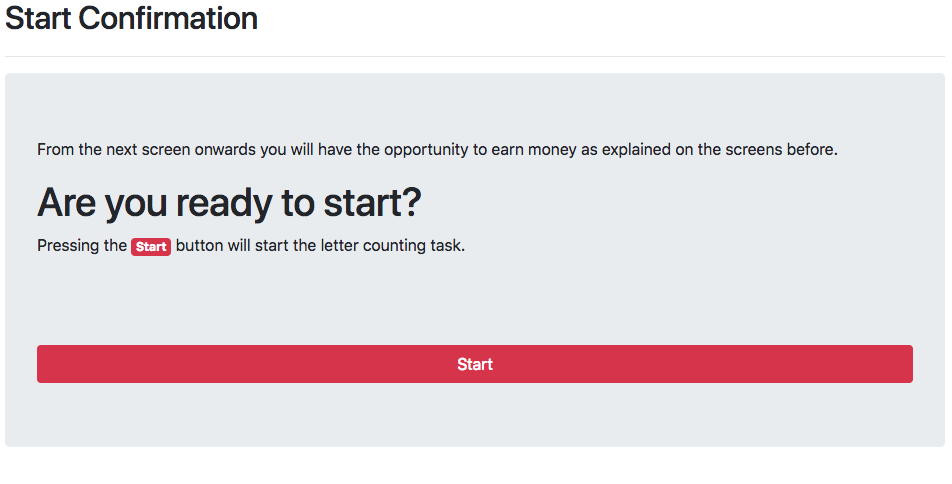
\includegraphics[width = 1.5in]{Screenshots/009-174-Start-RET.png}} &
\subcaptionbox{RET Screen\label{10}}{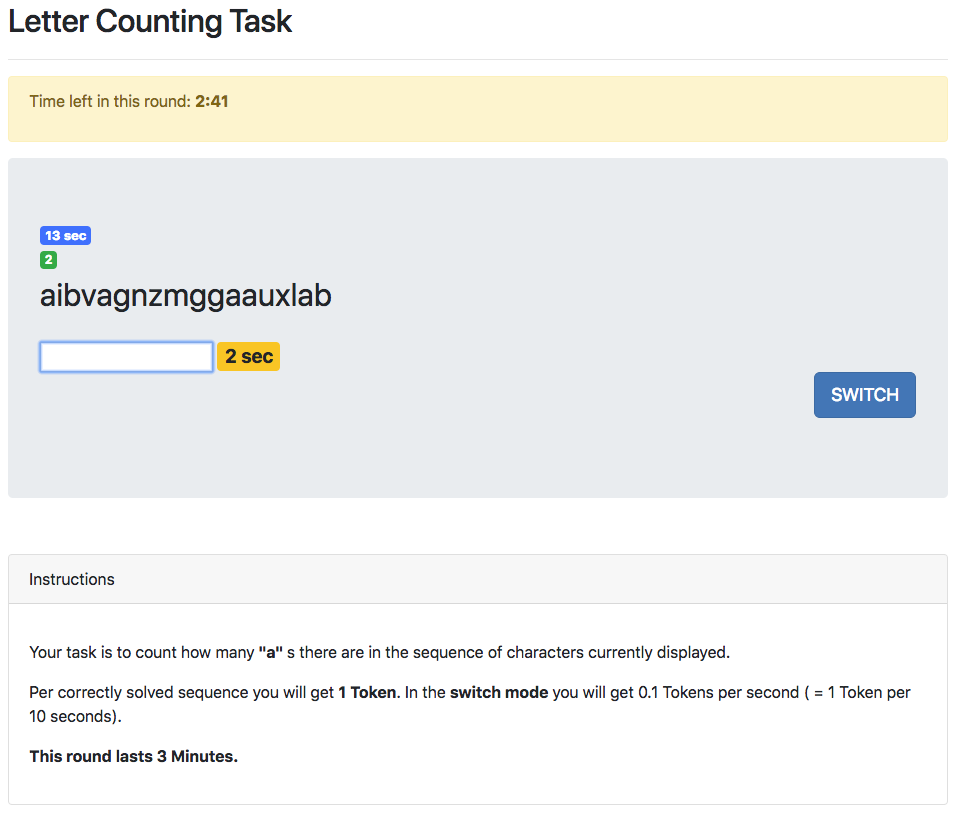
\includegraphics[width = 1.5in]{Screenshots/010-174-RET-1-2.png}} \\
\subcaptionbox{RET Switch Mode\label{11}}{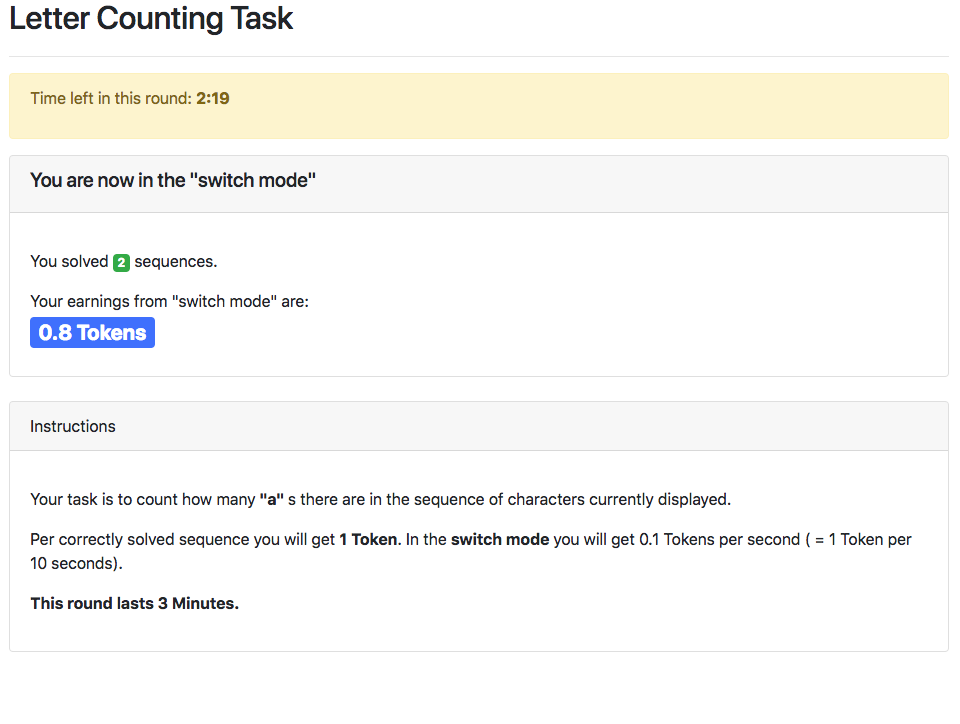
\includegraphics[width = 1.5in]{Screenshots/010-174-RET-2-2.png}} &
\subcaptionbox{RET Feedback Benchmarking\label{12}}{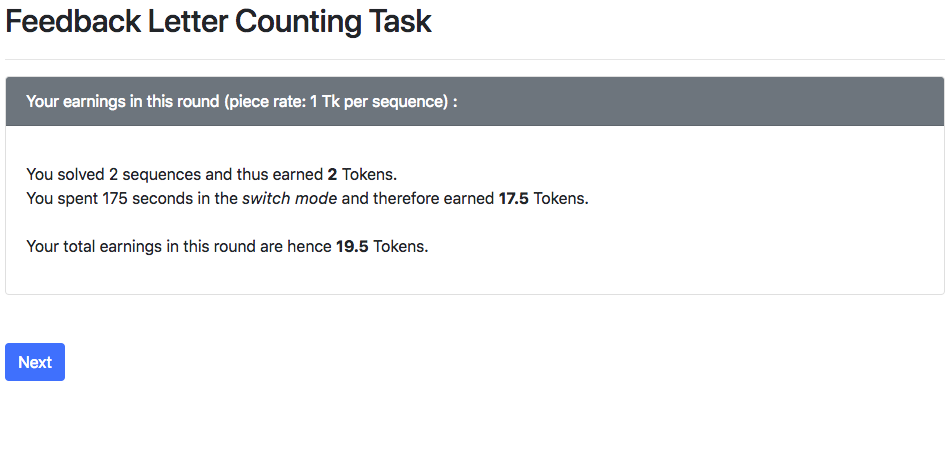
\includegraphics[width = 1.5in]{Screenshots/012-174-Feedback_Low.png}}\\
\end{tabular}
}
\caption{Screenshot Selection}
\label{ax:screenshot_2}
\end{figure}

\begin{figure}
\centering
\resizebox{1\columnwidth}{!}{%
\begin{tabular}{cc}
\subcaptionbox{High Piece Rate Earning Instructions\label{13}}{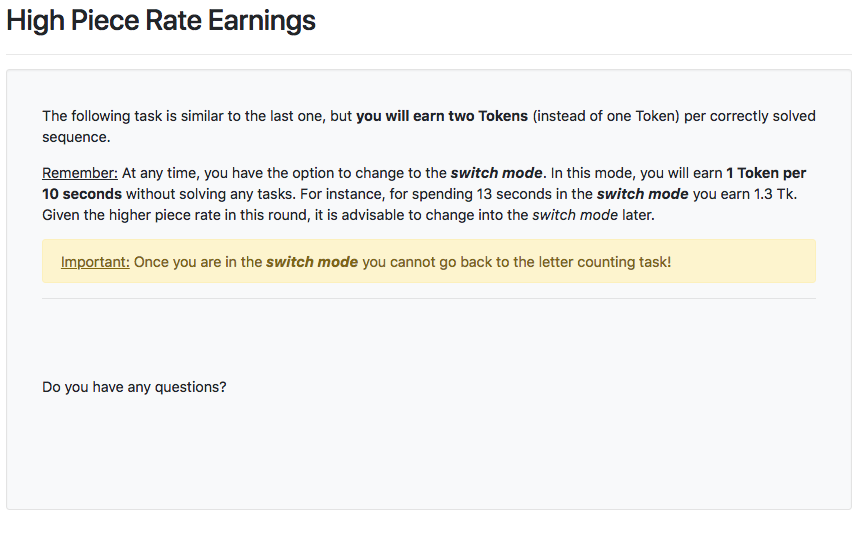
\includegraphics[width = 1.5in]{Screenshots/013-174-High-Instructions.png}} &
\subcaptionbox{Control Questions\label{14}}{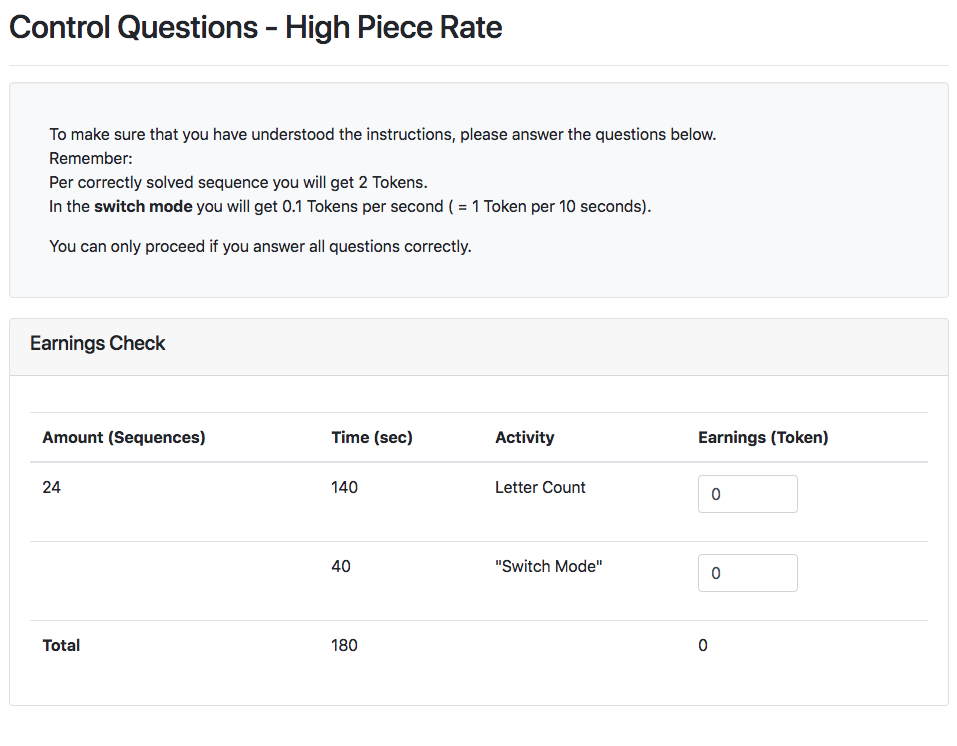
\includegraphics[width = 1.5in]{Screenshots/014-174-Control_Q_High-1-2.png}} \\
\subcaptionbox{Control Questions\label{15}}{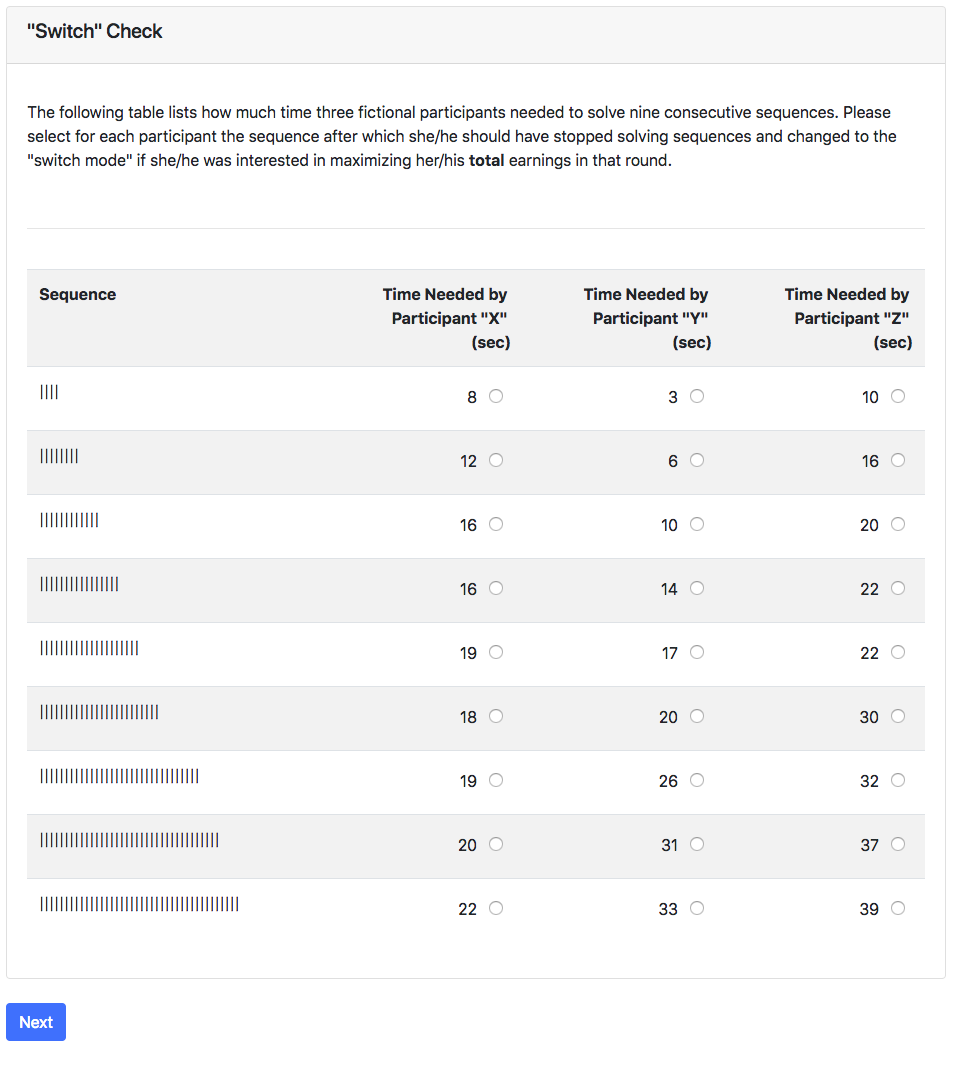
\includegraphics[width = 1.5in]{Screenshots/014-174-Control_Q_High-2-2.png}}&
\subcaptionbox{RET Feedback Benchmarking\label{16}}{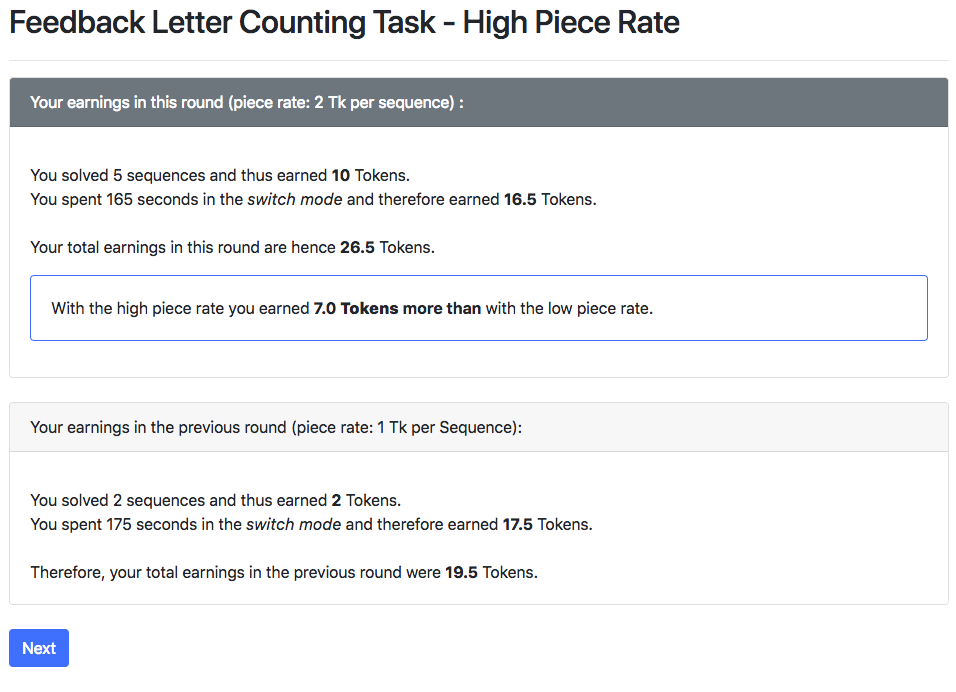
\includegraphics[width = 1.5in]{Screenshots/024-174-Feedback_High.png}} \\
\subcaptionbox{Competition Instructions\label{17}}{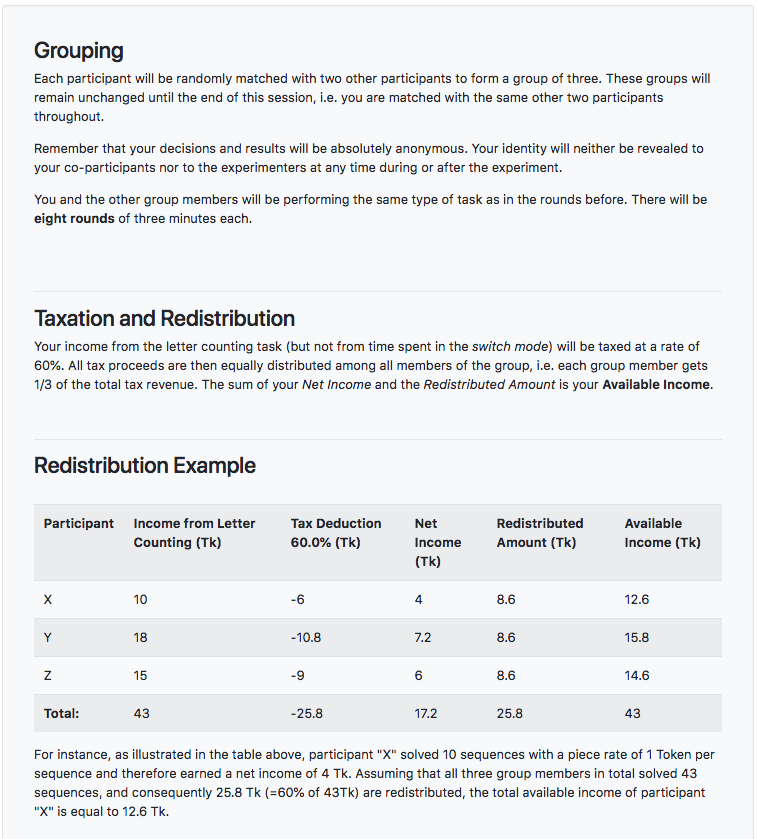
\includegraphics[width = 1.5in]{Screenshots/031-174-Grouping_and_Redi.png}} &
\subcaptionbox{Investment Instructions\label{18}}{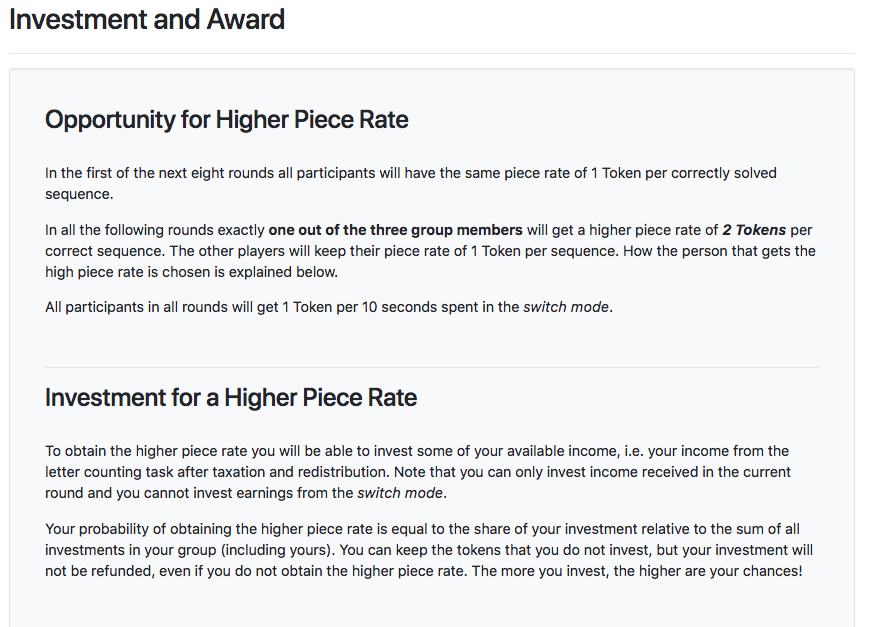
\includegraphics[width = 1.5in]{Screenshots/032-174-Investment_Instructions-1-2.png}}\\
\end{tabular}
}
\caption{Screenshot Selection}
\label{ax:screenshot_3}
\end{figure}

\begin{figure}
\centering
\resizebox{1\columnwidth}{!}{%
\begin{tabular}{cc}
\subcaptionbox{Structure of Experiment Screen\label{19}}{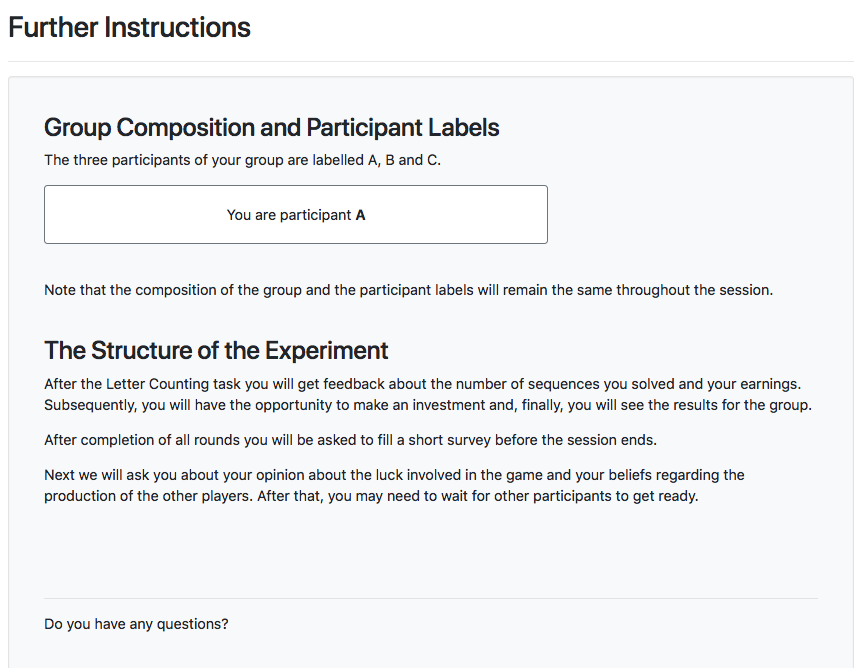
\includegraphics[width = 1.5in]{Screenshots/033-174-Structure.png}} &
\subcaptionbox{Fairness Questionnaire\label{20}}{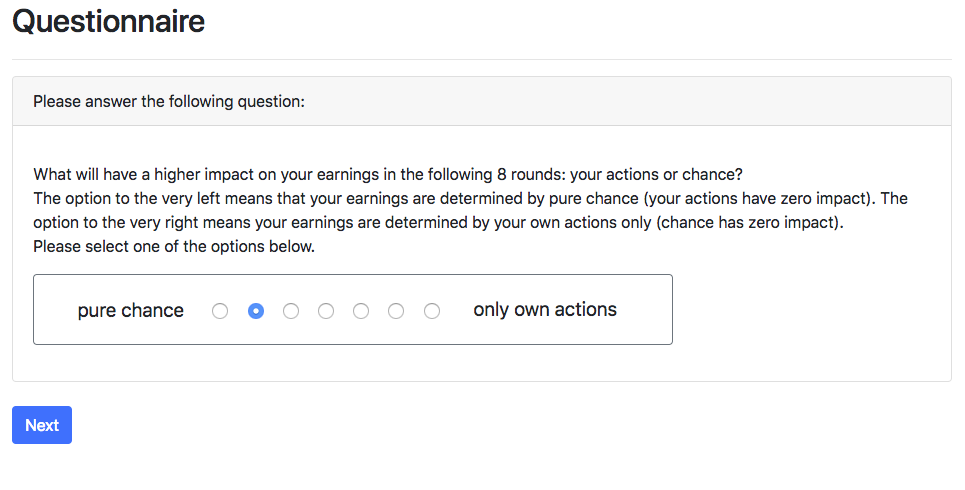
\includegraphics[width = 1.5in]{Screenshots/034-174-Fairness_Q_Begin.png}} \\
\subcaptionbox{Round Marker Screen\label{21}}{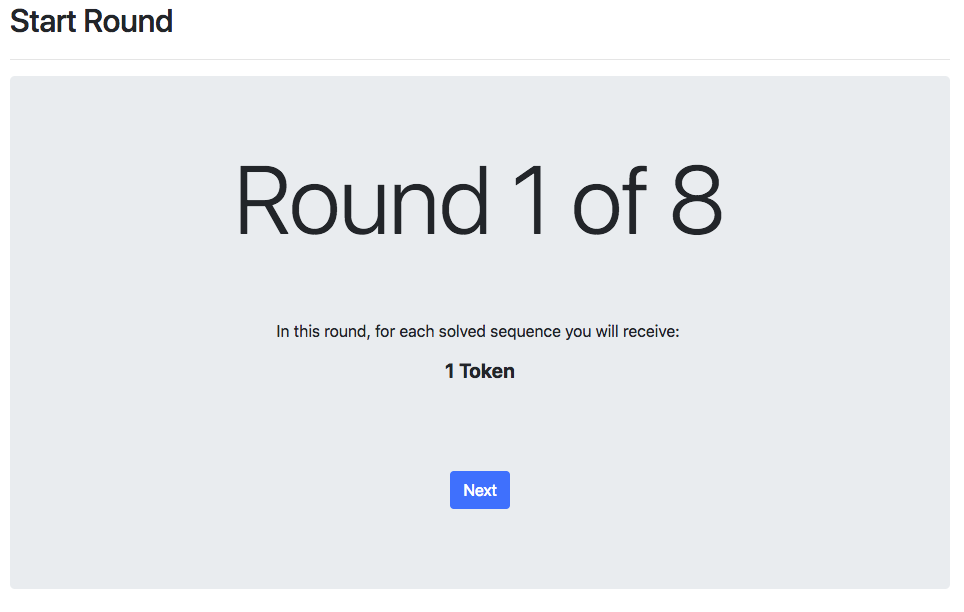
\includegraphics[width = 1.5in]{Screenshots/035-174-RoundStart.png}}&
\subcaptionbox{Production Beliefs Elicitation screen\label{22}}{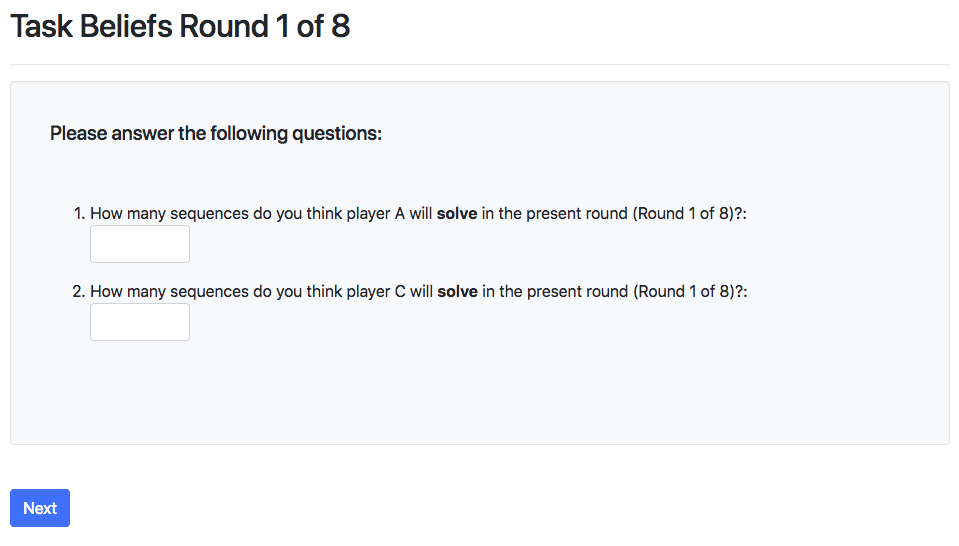
\includegraphics[width = 1.5in]{Screenshots/036-174-Beliefs_Prod.png}} \\
\subcaptionbox{RET Feedback Screen\label{23}}{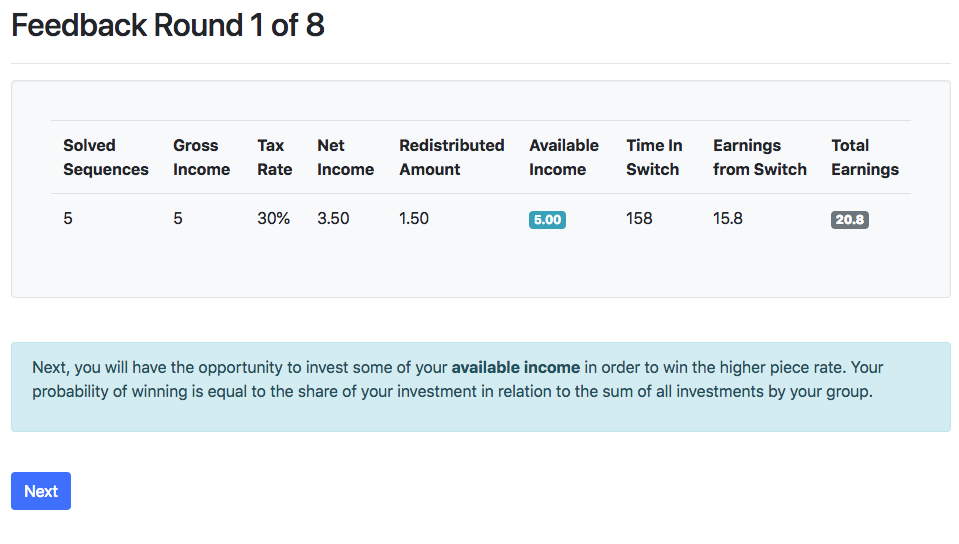
\includegraphics[width = 1.5in]{Screenshots/041-174-Feedback-RET.png}} &
\subcaptionbox{Investment Beliefs Elicitation\label{24}}{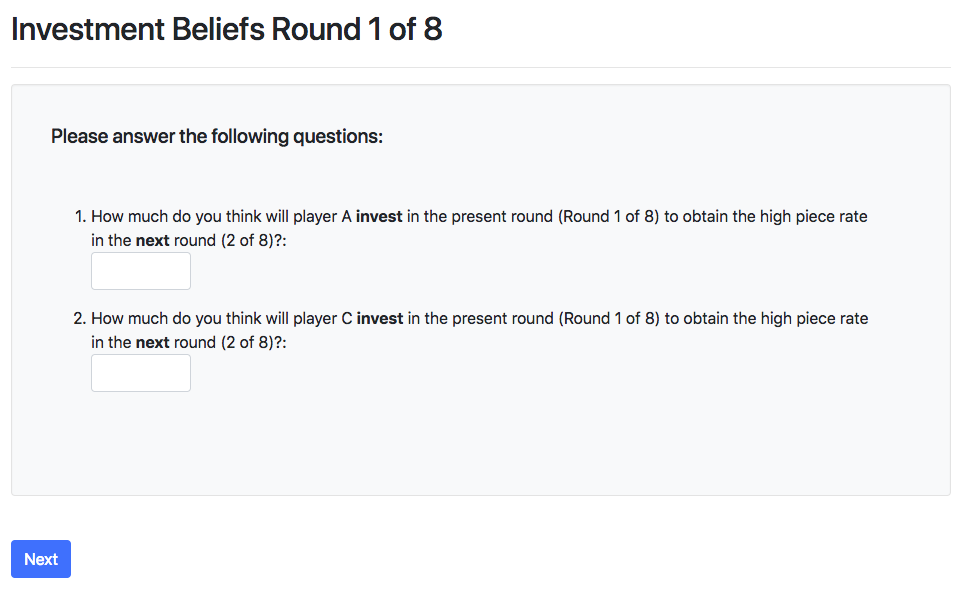
\includegraphics[width = 1.5in]{Screenshots/042-174-Beliefs_Investment.png}}\\
\end{tabular}
}
\caption{Screenshot Selection}
\label{ax:screenshot_4}
\end{figure}


\begin{figure}
\centering
\resizebox{1\columnwidth}{!}{%
\begin{tabular}{cc}
\subcaptionbox{Investment Screen\label{25}}{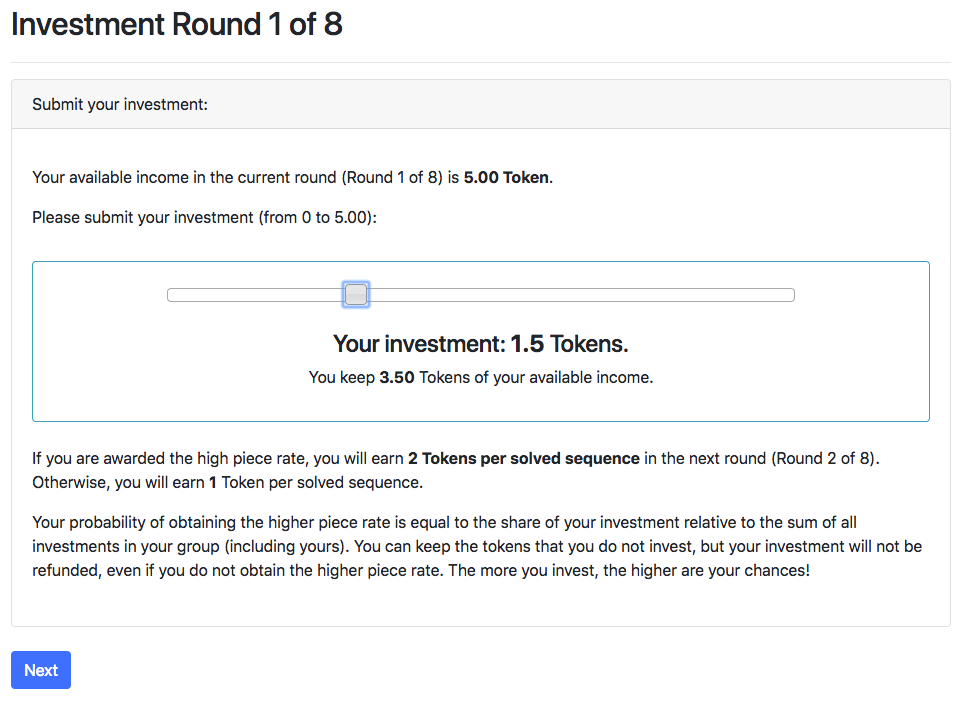
\includegraphics[width = 1.5in]{Screenshots/043-174-Investment.png}} &
\subcaptionbox{Investment Feedback Screen\label{26}}{\includegraphics[width = 1.5in]{Screenshots/045_174-Results.png}} \\
\subcaptionbox{Control Questions Marker Screen\label{28}}{\includegraphics[width = 1.5in]{Screenshots/166-174-Final_Q_Start.png}} &
\subcaptionbox{MLP Instructions\label{33}}{\includegraphics[width = 1.5in]{Screenshots/169-174-Instructions-MPL.png}}\\
\subcaptionbox{MLP Screen\label{34}}{\includegraphics[width = 1.5in]{Screenshots/171-174-Results-MPL.png}} &
\subcaptionbox{Demographics Questionnaire\label{36}}{\includegraphics[width = 1.5in]{Screenshots/172-174-Demographics.png}}\\
\end{tabular}
}
\caption{Screenshot Selection}
\label{ax:screenshot_5}
\end{figure}



\end{appendices}

%\input{literatur}
\bibliography{References}
\bibliographystyle{humannat}
%\printbibliography

\end{document}
